% Options for packages loaded elsewhere
\PassOptionsToPackage{unicode}{hyperref}
\PassOptionsToPackage{hyphens}{url}
%
\documentclass[
]{book}
\usepackage{amsmath,amssymb}
\usepackage{iftex}
\ifPDFTeX
  \usepackage[T1]{fontenc}
  \usepackage[utf8]{inputenc}
  \usepackage{textcomp} % provide euro and other symbols
\else % if luatex or xetex
  \usepackage{unicode-math} % this also loads fontspec
  \defaultfontfeatures{Scale=MatchLowercase}
  \defaultfontfeatures[\rmfamily]{Ligatures=TeX,Scale=1}
\fi
\usepackage{lmodern}
\ifPDFTeX\else
  % xetex/luatex font selection
\fi
% Use upquote if available, for straight quotes in verbatim environments
\IfFileExists{upquote.sty}{\usepackage{upquote}}{}
\IfFileExists{microtype.sty}{% use microtype if available
  \usepackage[]{microtype}
  \UseMicrotypeSet[protrusion]{basicmath} % disable protrusion for tt fonts
}{}
\makeatletter
\@ifundefined{KOMAClassName}{% if non-KOMA class
  \IfFileExists{parskip.sty}{%
    \usepackage{parskip}
  }{% else
    \setlength{\parindent}{0pt}
    \setlength{\parskip}{6pt plus 2pt minus 1pt}}
}{% if KOMA class
  \KOMAoptions{parskip=half}}
\makeatother
\usepackage{xcolor}
\usepackage{longtable,booktabs,array}
\usepackage{calc} % for calculating minipage widths
% Correct order of tables after \paragraph or \subparagraph
\usepackage{etoolbox}
\makeatletter
\patchcmd\longtable{\par}{\if@noskipsec\mbox{}\fi\par}{}{}
\makeatother
% Allow footnotes in longtable head/foot
\IfFileExists{footnotehyper.sty}{\usepackage{footnotehyper}}{\usepackage{footnote}}
\makesavenoteenv{longtable}
\usepackage{graphicx}
\makeatletter
\def\maxwidth{\ifdim\Gin@nat@width>\linewidth\linewidth\else\Gin@nat@width\fi}
\def\maxheight{\ifdim\Gin@nat@height>\textheight\textheight\else\Gin@nat@height\fi}
\makeatother
% Scale images if necessary, so that they will not overflow the page
% margins by default, and it is still possible to overwrite the defaults
% using explicit options in \includegraphics[width, height, ...]{}
\setkeys{Gin}{width=\maxwidth,height=\maxheight,keepaspectratio}
% Set default figure placement to htbp
\makeatletter
\def\fps@figure{htbp}
\makeatother
\setlength{\emergencystretch}{3em} % prevent overfull lines
\providecommand{\tightlist}{%
  \setlength{\itemsep}{0pt}\setlength{\parskip}{0pt}}
\setcounter{secnumdepth}{5}
\usepackage{booktabs}
\usepackage{booktabs}
\usepackage{longtable}
\usepackage{array}
\usepackage{multirow}
\usepackage{wrapfig}
\usepackage{float}
\usepackage{colortbl}
\usepackage{pdflscape}
\usepackage{tabu}
\usepackage{threeparttable}
\usepackage{threeparttablex}
\usepackage[normalem]{ulem}
\usepackage{makecell}
\usepackage{xcolor}
\ifLuaTeX
  \usepackage{selnolig}  % disable illegal ligatures
\fi
\usepackage[]{natbib}
\bibliographystyle{plainnat}
\usepackage{bookmark}
\IfFileExists{xurl.sty}{\usepackage{xurl}}{} % add URL line breaks if available
\urlstyle{same}
\hypersetup{
  hidelinks,
  pdfcreator={LaTeX via pandoc}}

\author{}
\date{\vspace{-2.5em}}

\begin{document}

{
\setcounter{tocdepth}{1}
\tableofcontents
}
\chapter*{}\label{section}
\addcontentsline{toc}{chapter}{}

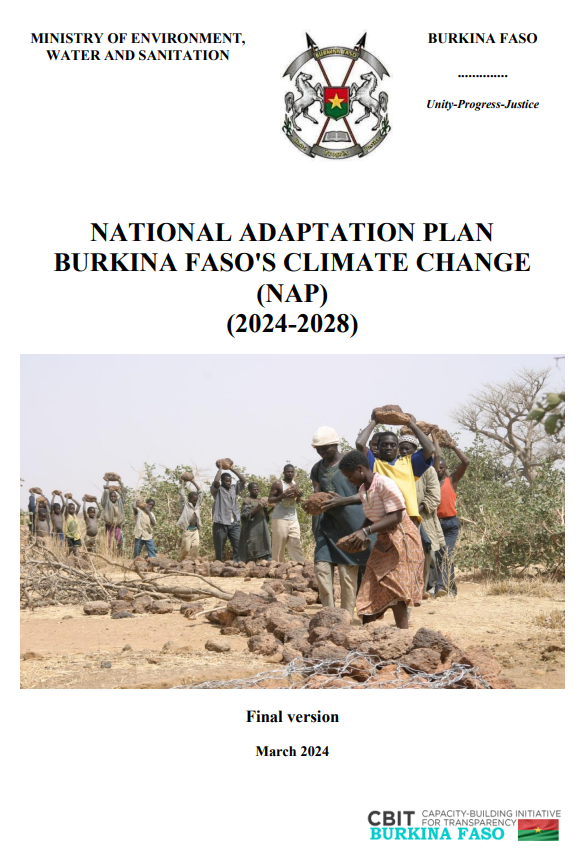
\includegraphics[width=6.25in,height=\textheight]{Figures and Photos/Cover Page.PNG}

\chapter*{Preliminaries}\label{preliminaries}
\addcontentsline{toc}{chapter}{Preliminaries}

\section*{Acronyms and abbreviations}\label{acronyms-and-abbreviations}
\addcontentsline{toc}{section}{Acronyms and abbreviations}

2IE : International Institute of Water and Environmental Engineering

ABN : Niger Basin Authority

ABV : Volta Basin Authority

ALG : Liptako Gourma Authority

ANAM : National Meteorological Agency

AND/FVC : Designated National Authority of the Green Climate Fund

APF : Wildlife Protected Areas

ASECNA : Agency for the Safety of Air Navigation in Africa and Madagascar

BAD : African Development Bank

EIB : European Investment Bank

IDB : Islamic Development Bank

BEEMER : World Bank

CBIT : Capacity-Building Initiative for Transparency

CBD : Convention on Biological Diversity

CDN : Nationally Determined Contributions

CESD : Environment and Sustainable Development Committee

ECOWAS : Economic Community of West African States

ESC/DRS : Water \& Soil Conservation/Defense Soil Restoration

CIFOR : International Center for Forestry Research

CILSS : Inter-State Committee for Drought Control in the Sahel

CIRDES : International Centre for Research and Development on Subhumid Livestock

CLD : Convention to Combat Desertification

CMIP : Project for Inter Comparison of Coupled Models

CNACC : National Committee on Climate Change

CNRA : National Center for Atmospheric Research

CNRST : National Center for Scientific and Technological Research

CNSF : National Centre for Forest Seeds

CONASUR : National Council for Emergency Relief and Rehabilitation

COP : Conference Of Parties

CRES : African Centre for Scientific Research and Training

CTS : Technical Monitoring Committee

ERDG : Directorate-General for Water Resources

EMOFA-B : Implementing Entity of the Climate Change Adaptation Fund of Burkina Faso

FAO : Food and Agriculture Organisation

EMF : Global Environment Facility

IFAD : International Fund for Agricultural Development

FIE : Environmental Intervention Fund

GCF : Green Climate Fund

GAR : Results-Based Management

LGB : General Circulation Models

GDDP : Global Daily Down scaled Projections

TDM : Sustainable Land Management

GHG : Greenhouse Gases

GGGI : Global Green Growth Institute

ICRISAT : International Crops Research Institute for the Semi-Arid Tropics

IIASA : International Institute for Applied Systems Analysis

IISD : International Institute for Sustainable Development

INSD : National Institute of Statistics and Demography

IRD : Research Institute for Development

LEG : Least Experts Group

MARAH : Ministry of Agriculture, Animal Resources and Fisheries

MEEA : Ministry of Environment, Water and Sanitation

MEMC : Ministry of Energy, Mines and Quarries

MESRI : Ministry of Higher Education, Research and Innovation

NEPAD : New Partnership for Africa and Development

NEX : Nasa Earth Exchange

ODD : Sustainable Development Goals

CSOs : Civil Society Organizations

PA-SDT : Stabilization and Development of the Transition

PAGIRE : Action Plan for Integrated Water Resources Management

PAM : World Food Programme

NFP : National Forest Policy

NTFP : Non-timber forest products

GDP : Gross Domestic Product

LDC : Least Developed Countries

PNA : National Climate Change Adaptation Plan

PNDD : National Sustainable Development Policy

NEDFN : National Policy for the Sustainable Development of Livestock

NSDP : National Health Development Plan

NCB : National Environmental Policy

NCB : National Water Policy

PNG : National Gender Policy

PNGIS : National Integrated Drought Management Plan

HNHP : National Policy on Housing and Urban Development

PNHP : National Public Health Policy

NSTRP : National Policy for Scientific and Technological Research

SNP : National Health Policy

NANSP : National Food and Nutrition Security Policy

RMFNP : National Policy for Land Security in Rural Areas

UNDP : United Nations Development Programme (UNDP)

UNEP : United Nations Environment Programme

POSEN : Energy Sector Policy

PPP : Public-Private Partnerships

PRA : Regional Adaptation Plan

PS-EEA : Sectoral Policy ``Environment, Water and Sanitation''

PSRI : Sectoral Research and Innovation Policy

PST : Transport Sector Policy

PTF : Technical \& Financial Partners

REEB IV : Fourth Report on the State of the Environment in Burkina Faso

RGPH : General Population and Housing Census

NAS : Assisted natural regeneration

CSR : Corporate Social Responsibility

SDAU : Urban Development Master Plan

SEF : Sahelian Eco-Farm

NCCS : National Climate Change Learning Strategy

SNADDT : National Plan for Land Use Planning and Sustainable Development

SNAT : National Spatial Planning Plan

DCS : National Strategy for the Implementation of the Convention on Climate Change

SNEV : National Green Economy Strategy

SNG : National Gender Strategy

SNI : National Industrialization Strategy

SNRCRS : National Strategy for Soil Restoration, Conservation and Recovery

SONABEL : Burkinabè Electricity Company

SP/CNDD : Permanent Secretariat of the National Council for Sustainable Development

SP/CONASUR : Permanent Secretariat of the National Council for Emergency Relief and Rehabilitation

SSP : Shared Socioeconomic Pathways

TWITCH : Information and Communication Technologies

AU : African Union

WAEMU : West African Economic and Monetary Union

IUCN : International Union for Conservation of Nature

UNCCD : United Nations Convention to Combat Desertification

WASCAL : West African Science Service Center on Climate Change and Adaptation Land Use

\section*{Executive summary}\label{executive-summary}
\addcontentsline{toc}{section}{Executive summary}

All scenarios show that global warming of the earth will intensify and exceed 1.5°C or even 2°C by 2050, unless significant reductions in CO2 and other greenhouse gas emissions occur in the coming decades (IPCC, 2021). This situation necessitates the development and adoption of greater adaptation strategies for developing countries that are the most vulnerable.

Aware that issues related to climate change can compromise its socio-economic development, Burkina Faso adopted its National Climate Change Adaptation Plan (NAP) in 2015. This strategic document, which is perfectly aligned with the country's current policies, has made it possible in its implementation to prevent and limit the negative consequences of climate change on its development in the medium and long term.

Planned for a period of 5 years (2015-2020), the NAP was evaluated in 2021 in order to address shortcomings and strengthen achievements for the years to come. The evaluation was carried out in a participatory manner with the actors of the sectors concerned by the NAP through an administrative decision setting up a team for the evaluation called the ``Technical Working Group''. At the end of the analysis, it appears that of the 143 actions planned, 96 actions have been carried out or are in the process of being carried out, i.e.~a rate of 77\% compared to 47 actions that have not started to start, i.e.~a rate of 33\%. Of the 77\% of the actions mentioned, 38\% have been completed and 29\% are in progress.

The development of an NAP is essential for countries to address climate change and ensure sustainable development. However, the evolution of the climate and the socio-economic context means that the priorities and challenges addressed may evolve from one NAP to another, hence the interest of this NAP, the formulation and implementation of which is based on the following principles: national ownership, empowerment of actors, results-based management, coherence of interventions, sustainability of interventions, gender mainstreaming and social inclusion,equity and partnership.

The vision of the NAP is: Burkina Faso manages its economic and social development more effectively through the implementation of planning mechanisms and measures that take into account resilience and adaptation to climate change by 2050.The overall objective of the NAP is to strengthen the resilience of people and ecosystems to climate change for inclusive and sustainable growth in Burkina Faso. Specifically, it is about:

\begin{itemize}
\item
  strengthen the adaptive capacities of people and ecosystems;
\item
  ensure the systematic integration of climate change adaptation into planning and budgeting at the national and local levels;
\item
  improve the mobilization of climate change adaptation finance;
\item
  promote research and development, local knowledge, know-how and endogenous best practices related to climate resilience, taking into account gender equality;
\item
  improving the governance of climate change adaptation
\end{itemize}

In addition to droughts and floods, the new challenges to be integrated into this NAP are heat waves, the late onset of the rainy season and its early end. The current NAP covers a period of 5 years (2024-2028) and will be implemented in a participatory manner with state and non-state actors.

In this NAP, three climate change scenarios have been identified: Shared Socioeconomic Pathways (SSPs; SSP1-2.6; SSP2-4.5 and SSP5-8.5) and two future periods (2021-2050: near future; 2051-2080: distant future) were considered with the reference period from 1985 to 2014. Climate observations in Burkina Faso reveal that in the near future, the northern part of the country could experience a significant early onset of the rainy season with a more pronounced trend in the SSP5-8.5 scenario. In the distant future, most parts of the West could experience a significant delay in precipitation of up to 5 days. Models predict an increase in the length of the rainy season in the near and distant future. An increase in precipitation is also expected. This increase is significant in all regions with a 95\% probability. The increase is more pronounced at the end of the century and in the high-emission scenario (SSP5-8.5). This scenario shows an increase of more than 20\%, especially in the northern part of the country, for the period 2051-2080. In the optimistic scenario (SSP1-2.6), the country could see a minimum increase of around 5\% for both periods. However, an increase in evapotranspiration is expected in the same proportion as that of precipitation. Current projections of water availability in Burkina Faso confirm the uncertainty of the resource regardless of the emission scenario considered due to a likely increase in evapotranspiration. As a result, given the cross-cutting nature of water resources, all other sectors, in particular agriculture, livestock, fisheries, food security and energy, will also be adversely affected by water-related issues. The areas where the risks would be highest are the Sahel region, the North region and the North Central region. It should be noted that water resources, agriculture and livestock are vulnerable sectors of these climate risk factors.

For air temperature, it is expected to increase in Burkina Faso. The western and northern parts of the country will experience greater warming, but the northern parts will have a higher increase. In addition, there will be a significant increase in the number of heat stress days and the number of cooling days, mainly in the western part of the country.

Several adaptation measures and strategies have been developed to improve the population's resilience to the future impacts of climate change. The adaptation priorities of this NAP are consistent with PNDES II and the Action Plan for the Stabilization and Development of the Transition (PA-SDT).

The operationalization of the National Adaptation Plan is based on three (3) strategic axes: (i) strengthening the adaptation capacities of priority sectors; (ii) climate change adaptation research and development; and (iii) governance of climate change adaptation interventions.

The implementation of the adaptation strategies and measures developed in this NAP will enable Burkina Faso to strengthen the resilience of the population of Burkina Faso to the negative impacts of climate change.

The overall budget for the implementation of the PNA for the five (5) year execution period is estimated at: \textbf{Two hundred and eleven billion, two hundred and thirty-three million, eight hundred and seventy-nine thousand, nine hundred and twenty-four (211,233,879,924) FCFA} of which \textbf{two hundred and eleven billion, two hundred and six million, two hundred and fifty-nine thousand, eight hundred and ninety-eight (211,206,259,898) FCFA} will be financed by the national government, \textbf{twenty-four million nine hundred and sixty-one thousand five hundred (24,961,500 FCFA)} addressed to the partners and the remainder \textbf{two thousand six hundred and fifty-eight thousand and eighty (2,658,080 FCFA) is to be sought}.

\chapter{Introduction}\label{introduction}

The planet is facing a new source of pressure, a new challenge that is damaging all socio-ecological systems with the increase in the atmospheric concentration of greenhouse gases (GHGs) attributable to human activities, including deforestation and the misuse of fossil fuels. Successive reports of the Intergovernmental Panel on Climate Change (IPCC) (2013-2019-2021) are unequivocal on this subject. Indeed, they presented several evidences of the global warming trend, the melting of glaciers, the variation of precipitation patterns, the increase in the frequency or intensity of extreme events and the rise in sea level over the last decades and also demonstrated with fairly high confidence levels the influence of human activities in these climate imbalances.

In addition, they highlighted the negative impacts that climate variations cause on the most important socio-economic sectors of developed and developing countries, including the Least Developed Countries (LDCs) (IPCC, 2014).

While developed countries are showing signs of resilience to the effects of climate change, the situation is worrisome and even critical for LDCs and other developing countries, which, despite their low contribution to climate change, are among the most affected because of their weak response capacity.

Regardless of the GHG emission scenarios considered, all climate models predict an increase in global temperature over the next few decades at least. The 6th Assessment Report of the IPCC Working Group I ``Climate Science and Physics'' published in August 2021, projects a faster than expected temperature increase; it is expected to reach or even exceed the threshold of +1.5°C, the most ambitious objective of the Paris Agreement, around 2030, if urgent and drastic measures to reduce GHG emissions are not implemented (IPCC, 2021). Above 1.5°C, one of the high-risk consequences in West Africa is exposure to potentially deadly hot temperatures for more than 100 days per year (IPCC, 2021), which would exacerbate the disastrous consequences for the socio-economic development of all countries, particularly Burkina Faso whose economies are largely dependent on climate (Semde et al., 2021).

In the light of various scientific assessments, and given that climate change-related risks amplify development challenges for LDCs, countries Parties to the United Nations Framework Convention on Climate Change (UNFCCC) have recognized, through the Cancun Adaptation Framework and Decision 5/CP.17 adopted at COP17 in Durban, South Africa, reinforced by the Paris Agreement, the urgent need to develop and implement National Adaptation Plans (NAPs) has seen it as a means to facilitate effective adaptation planning in LDCs and other developing countries (LEG, 2012).

Two main objectives are pursued through the NAPs: (i) to reduce vulnerability to the impacts of climate change by building adaptive capacity, disaster risk reduction and resilience, and (ii) to coherently integrate climate change adaptation into relevant new or ongoing policies, programmes and work, in particular sustainable development planning processes and strategies, across relevant sectors and at different levels, as appropriate (UNFCCC, 2020).

It is in this context that Burkina Faso found it imperative to develop its NAP on the eve of COP 21 in 2015. This document constitutes the general framework of medium- and long-term actions for national efforts to adapt to climate change in the following sectors: (i) agriculture, (ii) livestock production, (iii) environment and natural resources, (iv) energy, (v) health, (vi) infrastructure and housing, (vii) women's associations, (viii) civil society organizations. As the deadline for the implementation of the first NAP is 5 years, the year 2021 should mark the beginning of a new phase, hence the justification for its revision. The revision process started with the evaluation in 2021 of the first NAP.

This NAP specifies a set of adaptation actions to be implemented over the next five years and will serve as a reference for any communal, regional and sectoral adaptation plans to climate change. It also describes the strategies to be prioritized to address the different priorities of adaptation, analysis and risk management and makes recommendations on the monitoring and evaluation framework that can feed into reporting under the enhanced transparency framework established by the Paris Agreement.

The methodological approach was participatory and iterative, taking into account adaptation priorities at the regional and municipal levels. First, a technical committee was set up to monitor, guide and ensure the quality of the deliverables and their validation. In addition, national and international experts were also mobilized for the production of basic documents such as the report on the evaluation of the first NAP, the vulnerability study in a pilot region, and climate projections. Finally, the deliverable produced was submitted to multi-stakeholder national validations to provide a consensus document.

This NAP document consists of four (4) parts structured as follows:

➢ The first part presents the national circumstances, takes stock of the implementation of the previous NAP, sets out the revision process and climate scenarios, analyses and identifies the gaps and shortcomings of the previous NAP, proposes palliative solutions, identifies new challenges and priorities, sets out the revision methodology based on the analysis of climate scenarios, identifying and assessing vulnerabilities by development sector to climate change;

➢ the second part sets out the guiding principles, vision and objectives of the NAP, assesses the costs and benefits of adaptation options, presents the methodology for integrating climate change adaptation into development policies and strategies and finally develops how to operationalize the NAP;

➢ the third part presents the implementation strategies envisaged for the NAP, highlighting the political and legal framework and institutional arrangements, the communication strategy adopted, the contribution of research and development and finally the strategy for mobilizing technical and financial resources. The country, in the innovation perspective of its revised NAP, has adopted the development of Regional Adaptation Plans (RAPs) to climate change, the main results of which for a region are presented in this section;

➢ the fourth part reports on the monitoring and evaluation and reporting framework on the implementation of the NAP as well as information on the process of its revision.

\chapter{National circumstances, review of the implementation of the first NAP, review process and climate projections}\label{national-circumstances-review-of-the-implementation-of-the-first-nap-review-process-and-climate-projections}

\section{National context for the revision of the NAP}\label{national-context-for-the-revision-of-the-nap}

In order to better understand the scope of this NAP, including the actions to be implemented, this section provides a targeted overview of the main biophysical and socio-economic characteristics of Burkina Faso. It focuses on information that is relevant to the adaptation process.

\subsection{Geographical and administrative location}\label{geographical-and-administrative-location}

Burkina Faso is a landlocked country in sub-Saharan Africa located in the heart of West Africa in the Niger River Loop area. It is located between 9°20' and 15°05' north latitude, 5°20' west longitude and 2°03' east longitude. It covers an area of 274,200 km². The country is bordered to the north and west by Mali, to the east by Niger, and to the south by Ivory Coast, Ghana, Togo and Benin. It stretches 625 km from north to south and 850 km from east to west. Burkina Faso is a landlocked country and depends on its neighbours (Togo, Benin, Ghana and Côte d'Ivoire) for port traffic.

Administratively, Burkina Faso is divided into 13 regions, 45 provinces, 351 departments or communes, and 8,228 villages. There are 49 urban communes, including Ouagadougou, the political capital, and Bobo-Dioulasso, the economic capital (Figure 1). Since 2004, Burkina Faso has embarked on a policy of decentralization with the aim of strengthening the capacity of local authorities to act through the creation of local authorities.

\begin{figure}
\centering
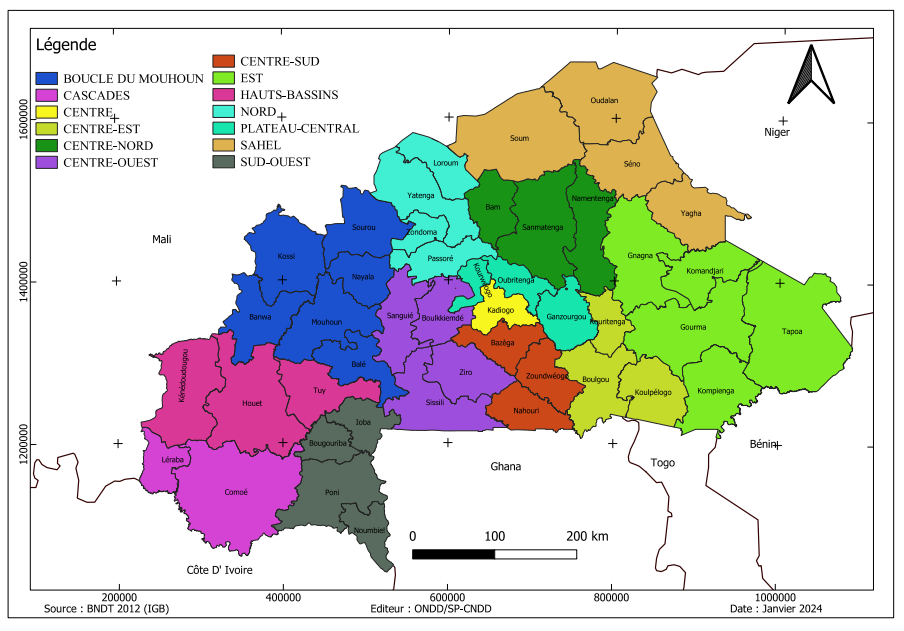
\includegraphics{Figures and Photos/Figure 1.png}
\caption{\textbf{Figure 1: Geographical and administrative situation of Burkina Faso}}
\end{figure}

\emph{Source: BNDT 2012 (IGB)}

\subsection{Socio-economic context}\label{socio-economic-context}

According to the report of the fifth General Population and Housing Census (RGPH, 2019), the country has about 20.5 million inhabitants with 51.7\% women and 48.3\% men, an increase of 7 million inhabitants compared to the last census carried out in 2006. The average annual population growth rate is 2.94\% (RGPH 2019). During the same period, the population density increased from 51.4 to 75.1 inhabitants/km2. The Burkinabe population is predominantly young; More than 77.9\% of the population is under the age of 35 and 51.8\% is under the age of 17.

Since 2016, the country has been experiencing a period of insecurity due to terrorist attacks. This situation has led to massive internal displacement of populations from insecure to relatively peaceful areas. A total of 1.99 million internally displaced persons (IDPs) have been registered by the Permanent Secretariat of the National Council for Emergency Relief and Rehabilitation (SP/CONASUR) as of 28 February 2023 compared to 1.94 million as of 31 January 2022, an increase of 3\%. Most of these displaced people, who left without their luggage, have no other means of survival than the untimely exploitation of natural resources in the host areas. In addition to these internally displaced persons, there are populations that traditionally migrate from arid climatic zones to more suitable and exploitable agricultural areas.

The majority of the Burkinabe population lives in a general state of poverty and constant impoverishment. The poverty rate increased from 41.4\% in 2018 to 43.2\% in 2021. The country is also characterized by a high illiteracy rate among people over the age of 15, standing at 61.7\% in 2018 (EHCVM 2018). The value of the Human Development Index (HDI) increased from 0.439 in 2017 to 0.449 in 2021 with a rank of 184th out of 191 countries ranked according to UNDP's Human Development Report (2021-2022).

Economically, the primary sector (agricultural and sylvo-pastoral activities) contributes more than 30\% to Burkina Faso's GDP and employs more than 80\% of the population (NANA, 2019). The fact that the largest part of the population depends on natural resources and rain-fed agriculture, climate change exacerbates rural poverty and increases anthropogenic greenhouse gas (GHG) emissions.

Although this sector of activity is very important for the country's economy, its high dependence on rainwater exposes it to the effects of climate change, calling into question the socio-economic development process of Burkina Faso (MERH, 2015). Hence the need to analyse the level of vulnerability of populations and to develop and implement appropriate adaptation strategies in order to strengthen their resilience to the adverse effects of climate change.

\subsection{Geophysical context}\label{geophysical-context}

The national territory of Burkina Faso is entirely drained by 3 international rivers, the Comoé, the Niger and the Volta, whose main tributaries are the Mouhoun and the Nakanbé (including Pendjari, Kompienga). For practical reasons of management and compliance with the principle of water resources management by basin, the national territory has been divided into 5 areas of competence for the management of water resources of river basins, resulting from a combination of the best possible administrative division (regions, provinces, municipalities) and the natural boundaries of the national river basins of the three (3) main international rivers. Water resources remain the country's main challenge, compromising its economic and social development (LAME, 2012).

\begin{figure}
\centering
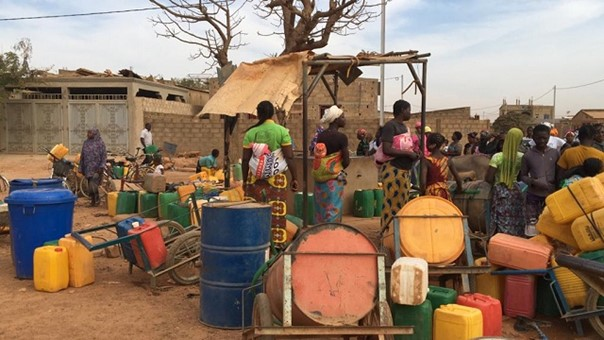
\includegraphics{Figures and Photos/Photo 1.png}
\caption{\textbf{Photo 1: View of drinking water shortages in Burkina Faso}}
\end{figure}

\emph{Source: Consultant for the revision of the NAP}

Burkina Faso has two main types of landscapes from the point of view of relief:

\begin{itemize}
\item
  The largest part of the country is covered by a peneplain. It forms a very slightly undulating relief with a few isolated hills in places, the last vestiges of a Precambrian massif. It is a rather monotonous landscape, with a soil very often coloured ochre by laterite.
\item
  The southwestern part of the country forms a sandstone massif. It is home to the highest point in the country: Ténakourou (749 m). The massif is bounded by very steep cliffs up to 150 m high: the cliffs of Banfora, the peaks of Sindou, etc.
\end{itemize}

The average altitude is 400 m and the difference between the two extreme points does not exceed 600 m. Burkina Faso is therefore a rather flat country, with some localized terrain accidents. This configuration is not conducive to efficient rainwater retention for agriculture and other uses.

From a pedological point of view, there are nine (09) soil classes in Burkina Faso:

\begin{itemize}
\item
  \textbf{Raw mineral soils} can be found on breastplates or surface formations that have not yet undergone or cannot undergo a soil evolution. These soils do not have a specific location. They are scattered throughout the country and represent three per cent of the total area of the country;
\item
  \textbf{Poorly developed soils} have a poorly differentiated profile in which the humus-rich horizon transitions to the original material by a more or less rapid transition. This slight change in the profile is due either to a slight impact of the climate or to the action of erosion which slows down the processes of alteration of materials at depth. Like raw mineral soils, they are found everywhere. But those with a basic facies are specific to certain regions such as Poni, Mouhoun; they cover 26\% of the total area;
\item
  \textbf{Vertisols} grow on basic rocks or on alluvium or colluvium from basic bedrock. They are deep soils (\textgreater{} 120 cm), dark in colour. However, these soils are poor in organic matter, nitrogen, phosphorus and potassium. Vertisols are found particularly in the provinces of Sourou, Nahouri, Sanguié, Boulgou, Gourma, and Zoundwéogo. They represent 6\% of the total area;
\item
  \textbf{Isohumic soils} are deep to medium-deep soils, growing on basic crystalline and metamorphic rocks or on calcareous sedimentary rocks. Their dominant hue is usually red due to the very extensive alteration of the minerals. Chemically, they are low in organic matter. They are rich in calcium and magnesium. Sometimes, sodium levels can be relatively high. Isohumic soils are represented in Burkina Faso by sub-arid brown soils located in the north of the country;
\item
  \textbf{Brown soils} are found in the western, south-west, north-central, northwestern and eastern parts of the country. They represent 6\% of the total area. These soils have a good mineral content, limited however by deficiencies in nitrogen, phosphorus and potassium;
\item
  \textbf{Within the class of soils with iron and manganese sesquioxides}, the subclass of \textbf{tropical ferruginous soils} is the most widespread (39\%). Its soils are characterized by a poverty of mineral elements;
\item
  \textbf{Ferralitic soils} develop on coarse sandstones (quartz-eyed sandstone) with a rainfall of between 1000 and 1200 mm. They are found in the west of the country, particularly in the provinces of Houet, Kénédougou, Comoé and in the southern part of the province of Mouhoun (Bondoukuy). They represent 2\% of the total area;
\item
  \textbf{Sodic or salsodic soils} are located in the Centre-South, Centre-North and East of the country. They occupy 5\% of the total area. They are compact soils with an unstable structure. The texture is medium to fine. They contain a significant amount of exchangeable sodium, which explains the instability of the structure;
\item
  \textbf{Hydromorphic soils} are found in the different regions of the country around major rivers (Mouhoun, Nakanbé, Nazinon), in the major riverbeds. They represent 13\% of the country's land area. In terms of importance, they are the third most important after ferruginous soils and poorly developed soils.
\end{itemize}

The relative poverty of the soil for agricultural activities has led producers to develop the production of organic manure.

\begin{figure}
\centering
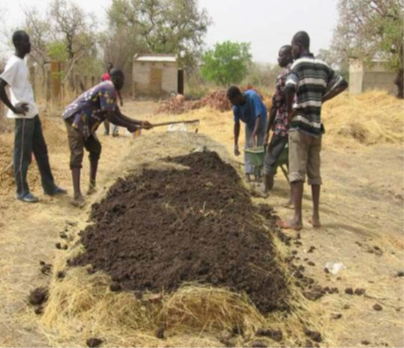
\includegraphics[width=6.73958in,height=\textheight]{Figures and Photos/Photo 2.png}
\caption{\textbf{Photo 2: View of the preparation of organic fertilization for the amendment of agricultural soils}}
\end{figure}

\emph{Source: Consultant for the revision of the NAP}

The territory of Burkina Faso is divided into four phytogeographical sectors of Burkina Faso (Fontès and Guinko, 1995): the strict Sahel, the sub-Sahel, the North Sudanian and the South Sudanian, marked by climatic conditions. According to the IFN2 report (MEEVCC, 2016), the types of forest formations encountered at the country level are: open forest, gallery forest, wooded savannah, shrub and grassy savannah, wooded steppe, shrub and grassy steppe, forest plantations and orchards. In particular, these forest formations are interspersed with agroforestry parks.

\subsection{Climate baseline}\label{climate-baseline}

Burkina Faso is subdivided into three distinct agro-climatic zones: the Sahelian zone in the north, the North Sudanian zone in the centre and the South Sudanian zone in the southwest. The boundaries of these subdivisions have migrated southward under the influence of climate change, as shown in Figures 2(a) and 2(b). The characteristics of each area are summarized in Table 1. The most significant climatic factor is rainfall, which decreases from north to south and is subject to strong seasonal and interannual variations, resulting in pronounced droughts or floods in some years with increasing frequency.

The very severe droughts of 1972-74 and 1983-84 left a strong mark on the country with their procession of disasters: decimated herds, poor harvests, famine, displaced populations, etc. These major natural calamities have encouraged national and international public awareness of the climate impacts and the great vulnerability of the Burkinabe population in particular and the Sahelian population in general. As a result of these events, sub-regional institutions such as the Inter-State Committee for the Fight against Drought in the Sahel (CILSS), headquartered in Burkina Faso, came into being on 12 September 1973.

\begin{figure}
\centering
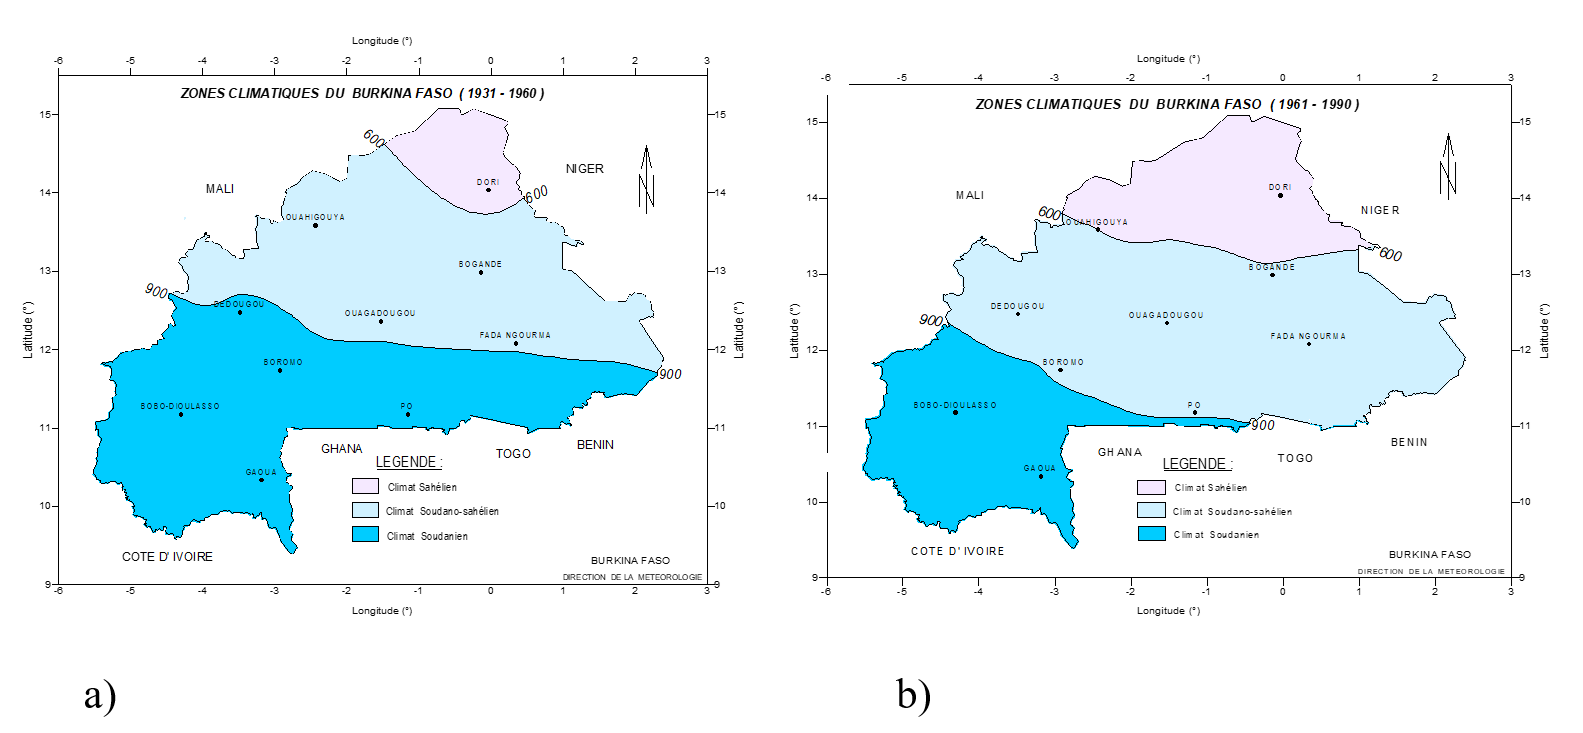
\includegraphics{Figures and Photos/Figure 2.png}
\caption{\textbf{Figure 2: Evolution of zones Eco-climatic studies of Burkina Faso between 1931 to 1960 (a) and between 1961 and 1990 (b)}}
\end{figure}

\emph{Source: National Meteorological Agency of Burkina Faso}

\begin{tabular}{>{}l|>{}l|>{}l|>{}l}
\hline
\multicolumn{4}{c}{Table 1: Characteristics of the climatic zones of Burkina Faso} \\
\cline{1-4}
Characteristics of climatic zones &   & Climatic Zones &  \\
\hline
NA & South Sudan & North Sudan & Sahelian\\
\hline
Annual rainfall & >1000 mm & 1000 to 600 mm & <600 mm\\
\hline
Length of the rainy season & 180-200 days & 150 days & 110 days\\
\hline
Number of rainy days & 85-100 days & 50-70 days & <45 days\\
\hline
Mean annual temperature & 27°C & 28°C & 29°C\\
\hline
Seasonal amplitude & 5°C & 8°C & 11°C\\
\hline
Humidity: & NA & NA & NA\\
\hline
  Dry season & 0.25 & 0.23 & 0.2\\
\hline
  Wet season & 0.85 & 0.75 & 0.7\\
\hline
Annual evaporation & 1800-2000 mm & 2600-2900mm & 3200-3500mm\\
\hline
\end{tabular}

\emph{Source: National Meteorological Agency of Burkina Faso}

The analysis of the current climate shows an upward trend in the average annual temperature over the three climatic zones, with an increase of 0.2°C per decade in Dori and 0.3°C per decade in Ouagadougou and Bobo-Dioulasso (Figure 3).

\begin{figure}
\centering
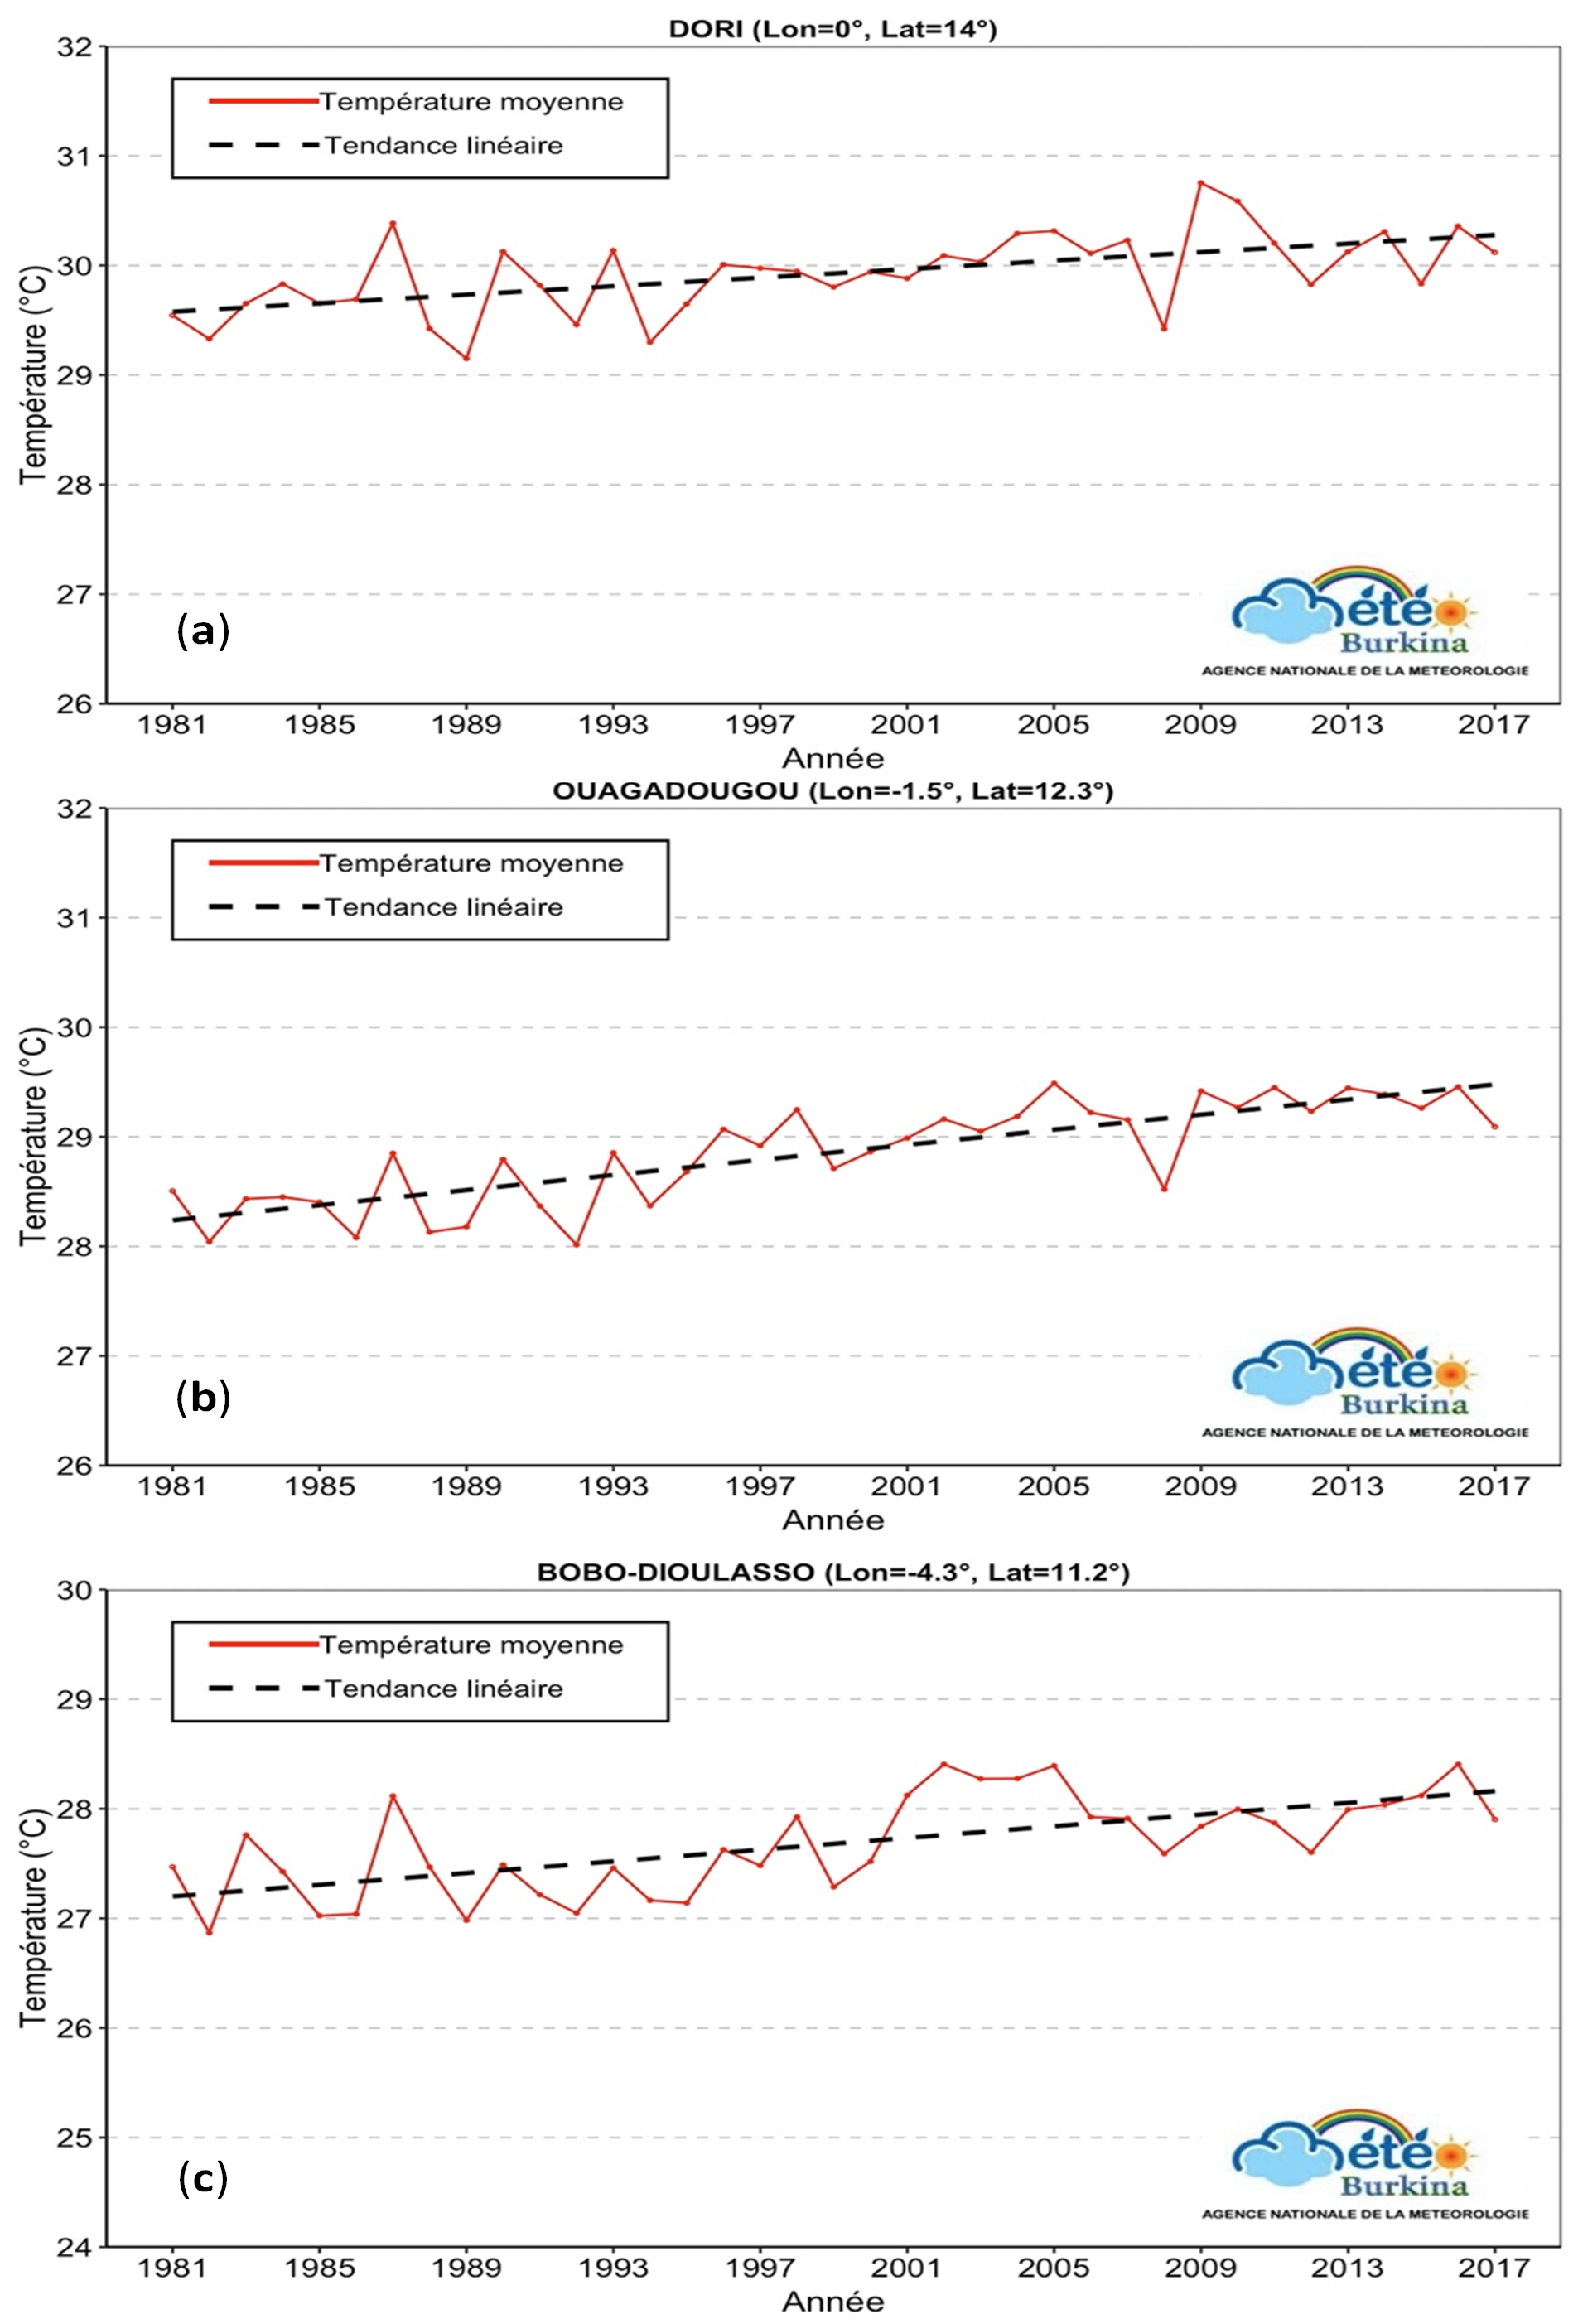
\includegraphics{Figures and Photos/Figure 3.png}
\caption{\textbf{Figure 3: Time series of the annual mean temperature over the period 1981-2018 for the station of Dori (a), Ouagadougou (b) and Bobo-Dioulasso (c)}}
\end{figure}

\emph{Source: National Meteorological Agency of Burkina Faso}

In terms of rainfall, taking the 1961-1990 normal as a reference in space, the 1981-2010 normal shows an increase in rainfall and shows a rise in the 600 mm and 900 mm isohyets towards the north. This increase is very pronounced in the last period 1990-2018 (Figure 4).

Precipitation indices show trends towards wetter conditions for annual precipitation (PRCPTOT), 1-day (RX1day) and 5-day (RX5days) maximum indices, extremely wet days (R99p). For the trend in the number of consecutive dry days (CDD), there is a slight decrease (\textless3 days/decade) corresponding to an increase in the number of rainy days in the eastern half of the country, while in the western half, there is a small increase in pockets of drought within the rainy season (3 days/decade).

\begin{figure}
\centering
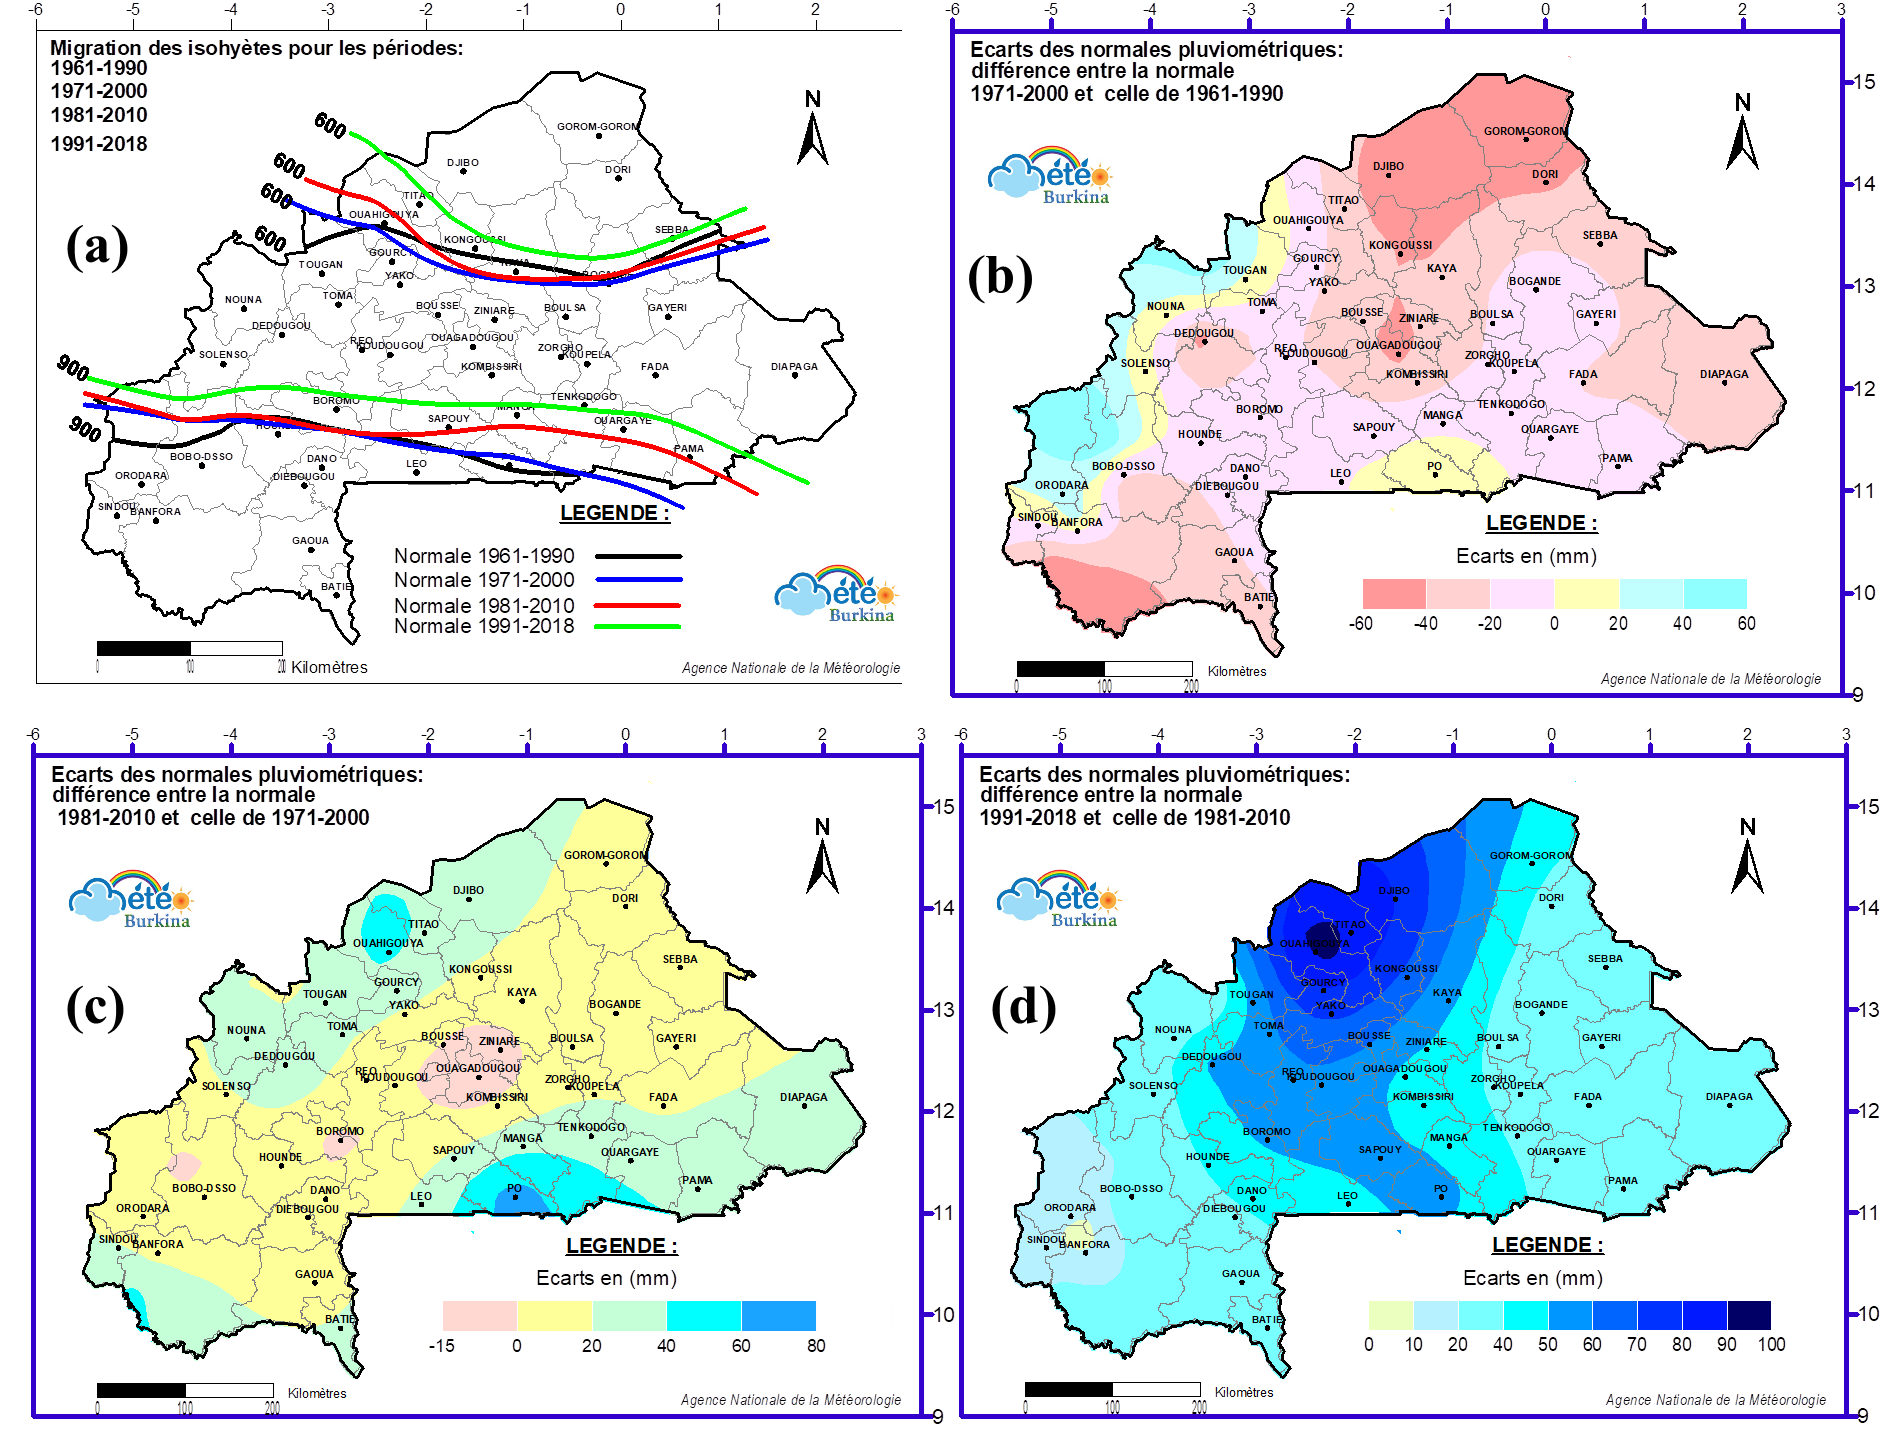
\includegraphics{Figures and Photos/Figure 4.png}
\caption{\textbf{Figure 4: Migration map of 600 mm and 900 mm isohyets for normals 1961-1990, 1971-2000, 1981-2010, and 1991-2018 (a). Grid points of climate projection data and the differences between these different periods: difference between 1971-2000 and 1961-1990 (b); Difference between 1981-2010 and 1971-2000 (c) and difference between 1991-2018 and 1981-2018 (d)}}
\end{figure}

\emph{Source: National Meteorological Agency of Burkina Faso}

\subsection{History of climate-related humanitarian emergencies from 1908 to the present day}\label{history-of-climate-related-humanitarian-emergencies-from-1908-to-the-present-day}

Burkina Faso is facing an upsurge in a series of climate-related disasters from 1908 to the present day (SP/CONASUR, 2012):

\begin{itemize}
\item
  repeated droughts in the years 1970-1973, 1983-1984, 1984-1985, 1991-1992, 1997-1998, 2003-2004 and 2011-2012 which led to loss of life and livestock, strong population migrations, and a significant drop in river levels;
\item
  recurrent floods in 1988, 1992, 1994, 2006, 2007, 2008, 2009, 2010, 2011 and 2012 with thousands of people homeless, thousands of ha of crops destroyed and millions of livestock decimated;
\item
  successive desert locust ravages for the periods 1908, 1948 and 1921, 1995, 1996 and 2004 which led to famine.
\end{itemize}

\section{Review of the implementation of the National Adaptation Plan (NAP)}\label{review-of-the-implementation-of-the-national-adaptation-plan-nap}

The evaluation was conducted for the period 2015-2020, with the support of the NAP Global Network and the International Institute for Sustainable Development (IISD). It was carried out in a participatory manner with the actors of the sectors concerned by the NAP through an administrative decision setting up a team for the evaluation called the ``Technical Working Group''.

The evaluation noted the progress made and the gains made, but also the shortcomings and challenges to be addressed in the new phase.

In terms of progress and achievements, the evaluation of the implementation of the development sectors targeted in the NAP shows that out of a total of 143 programmed actions, 96 actions have been carried out or are in the process of being implemented, i.e.~a rate of 67\% against 47 actions that have not started to get off the ground, i.e.~a rate of 33\%. Regarding the cross-cutting themes addressed (Gender and CSOs), gender did not carry out any activities and the activities carried out by CSOs could not be evaluated. However, it should be noted that many actions are being implemented in these two sectors, except that these actions were not included in the respective sectoral NAPs. These actions will be integrated into the new NAP.

\section{Analysis and identification of deficiencies that need to be reviewed for the NAP revision process}\label{analysis-and-identification-of-deficiencies-that-need-to-be-reviewed-for-the-nap-revision-process}

Among the difficulties and obstacles that have hindered the implementation of the previous NAP and that may be lessons for the new document, are: (i) the lack of awareness of the NAP by some actors of its implementation; (ii) the lack of institutional accountability for the actions of the NAP in conjunction with civil society and women's organizations; (iii) the non-operationalization of the institutional mechanism for monitoring and evaluation of the NAP; (iv) the inadequacy of gender mainstreaming in the monitoring of the implementation of NAP actions; (v) insufficient financial resources for the implementation of adaptation actions, (vi) the country's deleterious security situation and (vii) the COVID-19 pandemic.

In view of the diagnosis of the shortcomings and difficulties identified, palliative solutions have been proposed in order to improve the revised NAP.

\section{Elements of solutions to identified gaps and weaknesses}\label{elements-of-solutions-to-identified-gaps-and-weaknesses}

The positive actions (or initiatives) undertaken in favour of the implementation of the NAP have been as follows: (i) the institutionalisation of the NAP and NDC focal points which should ultimately make it possible to resolve the difficulties of monitoring actions at the sectoral level, (ii) the gradual inclusion of actions related to the NAP in the programmes of activities of certain ministerial departments, (iii) the development of the Institutional Capacity Building Programme in relation to the implementation of the NAP, (iv) the continuous capacity building of stakeholders on the NAP and the NDC.

A few points of recommendation have been formulated and to be taken into consideration for the future: (i) to promote the dynamism of a framework for consultation between the implementing actors and to hold periodic follow-up meetings; (ii) strengthen the capacities of implementing actors on strategies for mobilizing financial resources for the implementation of the NAP; (iii) align the NAP with the SDGs; (iv) ensure that the NAP is taken into account in development frameworks; (v) identify and create a database to facilitate the monitoring of civil society actions working in the fight against climate change and involve them in implementation; (vii) clearly define actions and their short-, medium- and long-term targets to facilitate monitoring and evaluation; (viii) strengthen the skills of the NAP focal points to facilitate the monitoring and reporting of the actions of their respective sectors in relation to the NAP; and (ix) develop and implement an NAP Communication Plan.

\section{Identification of emerging challenges and priorities}\label{identification-of-emerging-challenges-and-priorities}

While the development of an NAP is essential for countries to address climate change and ensure sustainable development, however, changes in the climate and socio-economic context mean that the priorities and challenges addressed may change from one NAP to another. In addition to droughts and floods, the new challenges to be integrated into this NAP are heat waves, the delay of the rainy season and its early end (SP/CNDD, 2023). The adaptation priorities of this NAP are in line with the main development axes of the National Economic and Social Development Plan (PNDES II; 2021-2025) which are: (1) consolidating resilience, security, social cohesion and peace; (2): deepening institutional reforms and modernizing public administration; (3): consolidating human capital development and national solidarity; (4) : boost sectors that are promising for the economy and jobs.

Finally, the NAP uses the new IPCC scenarios listed in its Assessment Report Number 6 (AR6) called the Shared Socio-economic Pathway (SSP), which offer more realistic results by combining socio-economic activities and radiative forcings.

\section{NAP review process}\label{nap-review-process}

The process of revising the NAP was led by the Ministry of the Environment and was the recruitment of a national consultant supported by international consultants. A Technical Monitoring Committee (STC) chaired by the Permanent Secretariat of the CNDD has been set up to provide strategic guidance and validate the methodology as well as the interim reports submitted by the consultants. Several semi-structured interviews were conducted with the various stakeholders, particularly the focal points of the ministerial departments. The national consultant also interviewed members of the LDC Expert Group on Climate Change (LEG), resource persons and carried out a documentary dig of climate resilience, sustainable development policies in general and Burkina Faso in particular. The LDC Expert Group's technical guides or guidelines for the National Adaptation Plan process have been judiciously used in this work.

Finally, the final document was validated by the CTS and then by a national workshop bringing together a wider audience.

Funding for this activity was provided by the United Nations Environment Programme (UN Environment) based in Nairobi through the Capacity-building Initiative for Transparency (CBIT) project.

\section{Analysis of climate projections}\label{analysis-of-climate-projections}

\subsection{General}\label{general}

As a party to the Paris Agreement, Burkina Faso has committed to reducing its greenhouse gas emissions and significant efforts have been made. The country's Nationally Determined Contribution (NDC), adopted in 2015 and revised in 2021, demonstrate the government's commitment to significantly reduce greenhouse gas emissions by 2040 with the support of its technical partners. To determine the climate vulnerability factors used in this NAP, the NASA Earth Exchange (NEX) Global Daily Downscaled Projections (GDDP) or NEX-GDDP dataset was used. This dataset comes from a statistical downscaling of general circulation models (GCMs) performed as part of Phase 6 of the Coupled Model Intercomparison Project (CMIP6) at a spatial resolution of 25 km (Thrasher et al., 2022).

In the previous NAP, scenarios A2, B1 and A1B were used for projections of future climate change for precipitation and temperature. Shared Socioeconomic Pathways (SSP) climate change scenarios are used to project the different climate impact factors listed in Table 2. PHS were developed to provide five distinct pathways on future socio-economic developments as they might unfold in the absence of explicit additional policies and measures to limit climate forcing, or to improve adaptive capacity (Riahi et al., 2017). SSP scenarios are used in the IPCC's Sixth Assessment Report for climate change projections. In this NAP, three PHCs (SSP1-2.6; SSP2-4.5 and SSP5-8.5) and two future periods (2021-2050: near future; 2051-2080: distant future) were considered. SSP1-2.6 roughly corresponds to the previous generation of RCP 2.6 scenarios with a radiative forcing of 2.6 W m-2 by the end of the century. It most closely reflects the 2°C goal of the Paris Agreement and is the highest priority scenario in the Sixth Assessment Report (AR6). It is followed by the ``average'' socioeconomic family SSP2-4.5 with a nominal radiative forcing of 4.5 W m-2 by 2100, roughly equivalent to the RCP-4.5 scenario. Finally, the SSP5-8.5 scenario marks the upper limit of the SSP scenario spectrum with a high reference scenario (business as usual) in a fossil fuel-intensive world in the XXITh century. It has a radiative forcing of 8.5 W m-2 by the end of the century, like the RCP8.5 scenario that preceded it.

For climate projections, the ``multi-model average set'' was used, which provides better performance than a single model. It is formed by combining a set of models with equal weights and has a higher probability of producing a better result than a single model (Sawadogo et al., 2019). It also performs better in terms of long-term climate change projections than any single model (Houghton et al., 2001). Nevertheless, 80\% of models must agree on the sign of changes to be considered robust changes (Fischer et al., 2014). The agreement of the models is shown in the figures as a pie chart. In addition, the average of the models should indicate that the projected change is statistically significant at the 95\% confidence level, based on a (Student's) test. Significant areas at the 95\% confidence level are represented in the figures as dots. We chose the period 1985-2014 as the reference period.

The various studies of vulnerability and impacts of climate change have made it possible to identify the different climate risk factors and their impacts on the different sectors of activity (Arisco et al., 2023; Ibrahim et al., 2014; Ouedraogo et al., 2012).

Table 2 shows the different climate risks identified for the NAP and the sectors of activity impacted.

\textbf{Table 2: Sectors of activity and climate risks associated with Burkina Faso}

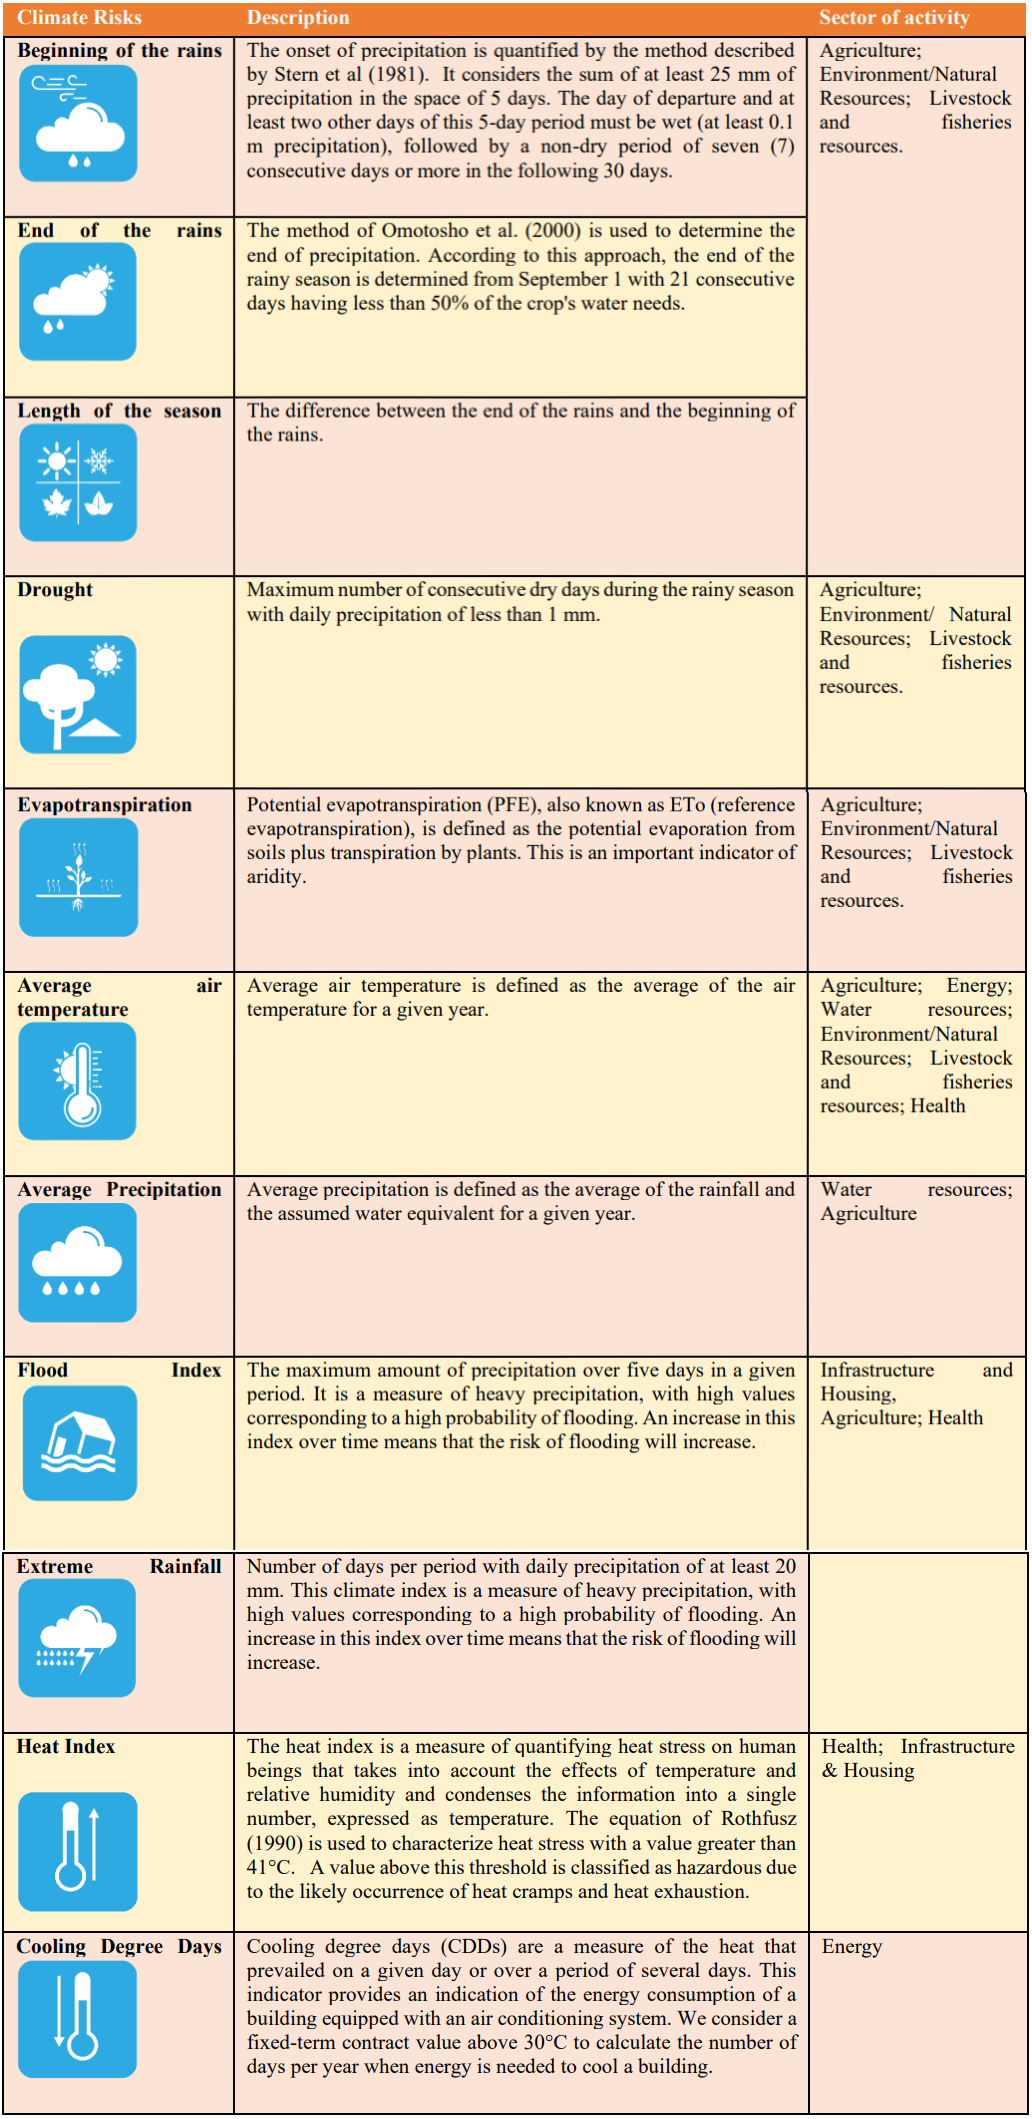
\includegraphics{Tables/Table 2.PNG}

\emph{Source: Burkina Faso Climate Vulnerability Study Report}

\subsection{Start, end and duration of the rainy season}\label{start-end-and-duration-of-the-rainy-season}

The overall average of the models projects a generally early onset of precipitation in the near and distant future over Burkina Faso (Figures 5 \& 6). In the near future, the northern part of the country could experience a significant early start to the rainy season and this is more pronounced in and in the SSP5-8.5 scenario. In the distant future, most parts of the West could experience a significant delay in precipitation of up to 5 days. However, there is a divergence between the models in terms of the sign of projection in the two periods. For example, 53\% of models predict an early onset date of precipitation, while 47\% show a late onset of precipitation under the SSP1-2.6 scenario and in the near future. In contrast to the date of the start of the rains, more than 80\% of the models agree with the sign of increasing rain stop both in the near future and in the future. This is also confirmed for the duration of the rainy season, where all models show a significant increase but there is less agreement between models, especially the SSP1-2.6 scenario. Overall, the country could experience a significantly longer rainy season in the coming years. This significant increase is more pronounced in the SSP5-8.5 model and at the end of the century. The length of the rainy season could also increase by 10 to 15 days, especially in the northern part of the country. In conclusion, farmers will need to adapt their cropping practices to expected changes in the onset and length of the rainy season to reduce crop losses and also use improved seeds to reduce the uncertainty associated with planting timing and the length of the rainy season.

The agreement of the models is shown in the figures as a pie chart. In addition, the average of the models should indicate that the projected change is statistically significant at the 95\% confidence level, based on a (Student's) test.

Significant areas at the 95\% confidence level are represented in the figures as dots.

\begin{figure}
\centering
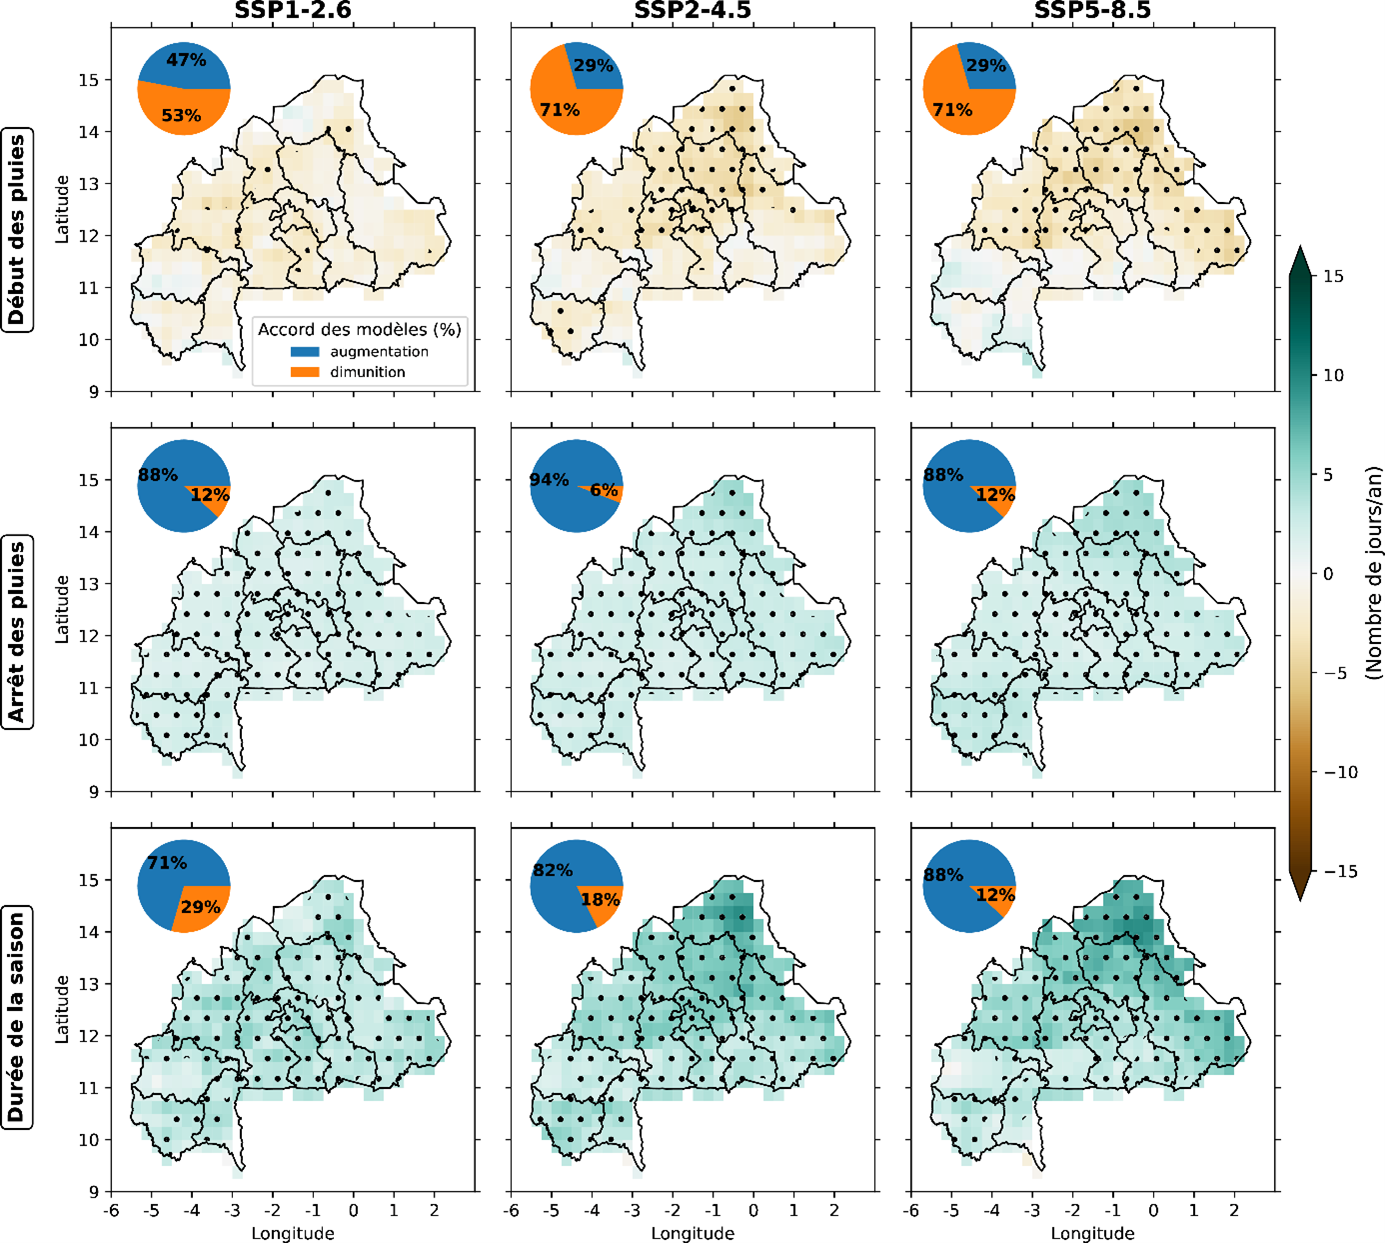
\includegraphics{Figures and Photos/Figure 5.png}
\caption{\textbf{Figure 5: Projected changes in the mean of all models of the onset, cessation and duration of precipitation over Burkina Faso under different shared socioeconomic pathways (SSPs) for the near future (2021-2050)}}
\end{figure}

\emph{Source: Consultant for the revision of the NAP}

The dots mark the areas where the changes are significant at the 95\% probability level. The pie chart in each case shows the percentage of agreement of the models on the country average.

\begin{figure}
\centering
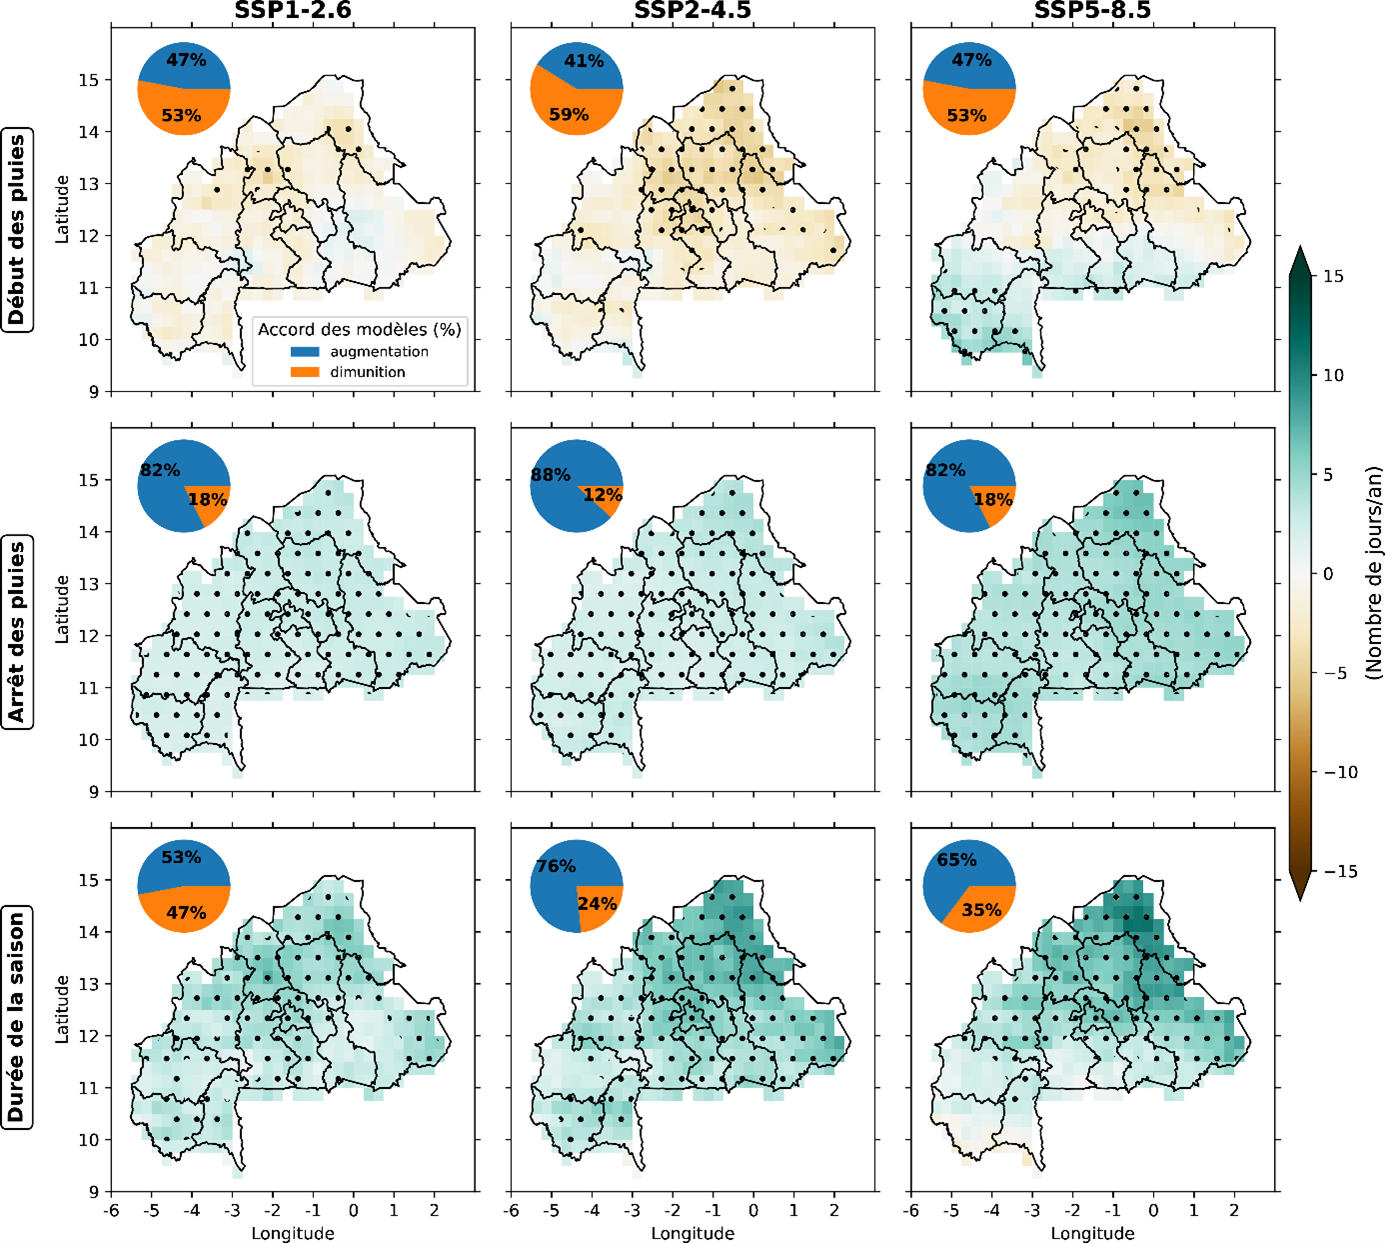
\includegraphics{Figures and Photos/Figure 6.png}
\caption{\textbf{Figure 6: Similar to Figure 5, but for the distant future (2051-2080)}}
\end{figure}

\emph{Source: Consultant for the revision of the NAP}

\subsection{Annual precipitation and evapotranspiration}\label{annual-precipitation-and-evapotranspiration}

About 80\% of the models predict an increase in precipitation in Burkina Faso in all scenarios and periods considered (Fig.7). This increase is significant in all regions with a 95\% probability. The increase is more pronounced at the end of the century and in the high emissions scenario (SSP5-8.5). This scenario shows an increase of more than 20\%, especially in the northern part of the country, for the period 2051-2080. In the optimistic scenario (SSP1-2.6), the country could see a minimum increase of about 5\% for both periods. Figure 7 shows the average inter-annual rainfall projection over Burkina Faso. This figure is obtained by aggregating all grid points in the Burkina Faso area. The shading in the figure indicates the minimum and maximum of the models. For each scenario, the model's ensemble average projects an increase in precipitation towards the end of the century with a maximum increase of about 20\%. However, the model shows a high temporal variability in the increase in precipitation for all scenarios and up to 2100. This means that precipitation can vary from year to year but is higher than the reference period (1985-2014). Despite the expected increase in rainfall in the country, a net decrease in water availability is expected due to increased evapotranspiration. The increase in evapotranspiration is consistent between models (Fig. 9). More than 80\% of models show that evapotranspiration increases in all scenarios and at all time periods. This increase is also evident in the SSP5-8.5 scenario and the end of the century. Under the SSP1-2.6 scenario, the country's evapotranspiration is expected to increase by at least 5\%. This increase could lead to lower soil moisture and more frequent and severe agricultural droughts. In addition, reduced water availability could affect off-season crops in the coming years and will have serious implications for drinking water management and irrigation. The increase in precipitation and evapotranspiration highlighted here is consistent with the IPCC6 assessment report (Paola et al., 2021).

There is a change in the average rainfall in Burkina Faso compared to the average of all models for the reference period (in black) and three SSPs (Shared Socioeconomic Pathways) scenarios (compared to 1985-2014): SSP1-2.6 (in blue), SSP2-4.5 (in green), and SSP5-8.5 (in red). The light color shaded around the reference period and the different SSPs indicates the minimum and maximum of the models.

\begin{figure}
\centering
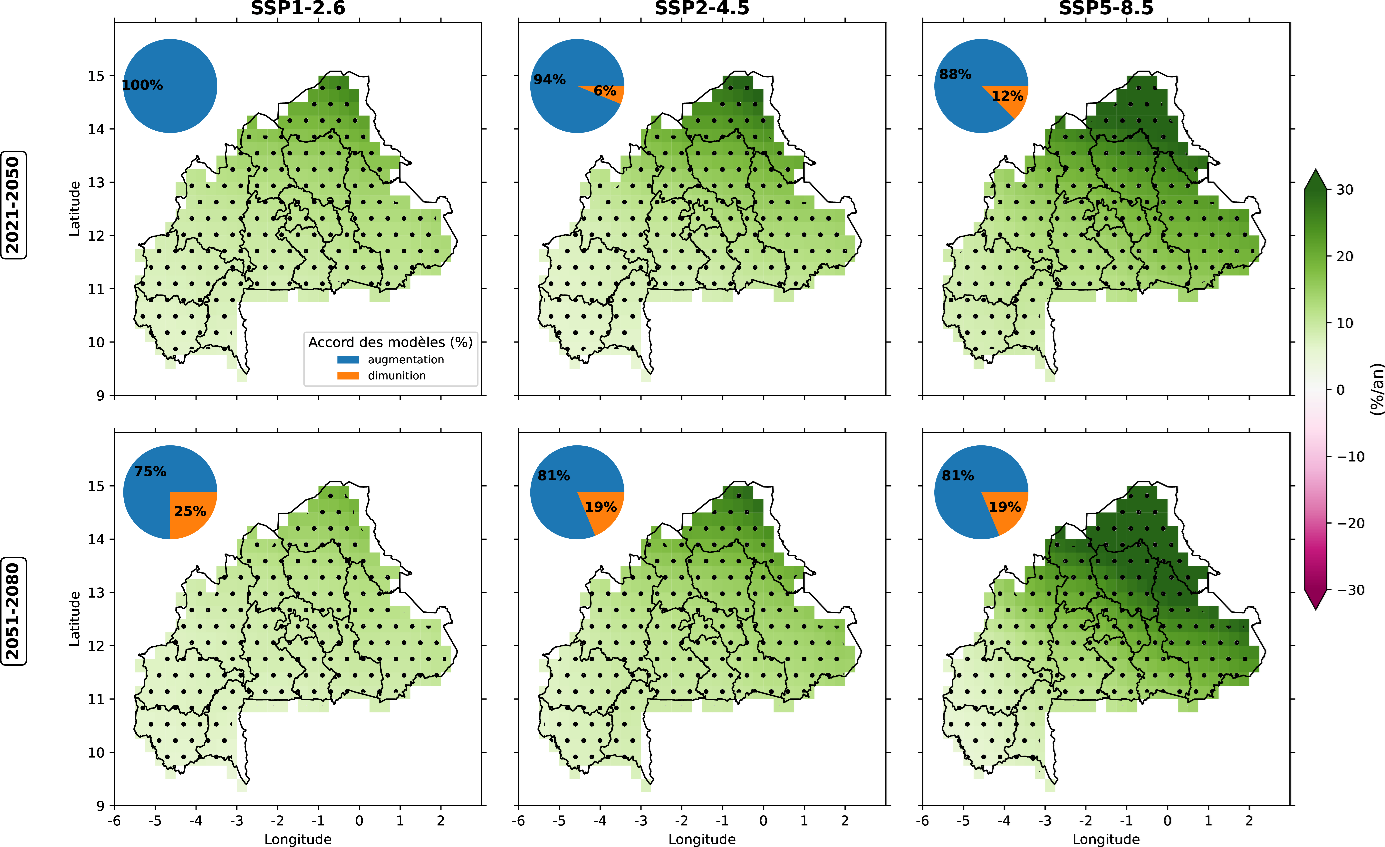
\includegraphics{Figures and Photos/Figure 7.png}
\caption{\textbf{Figure 7: Projected changes in the mean of all precipitation models over Burkina Faso under different shared socioeconomic pathways (SSPs) for the near (2021-2050) and distant (2051-2080) future}}
\end{figure}

\emph{Source: Consultant for the revision of the NAP}

The dots mark the areas where the changes are significant at the 95\% probability level. The pie chart in each case shows the percentage of agreement of the models on the country average.

\begin{figure}
\centering
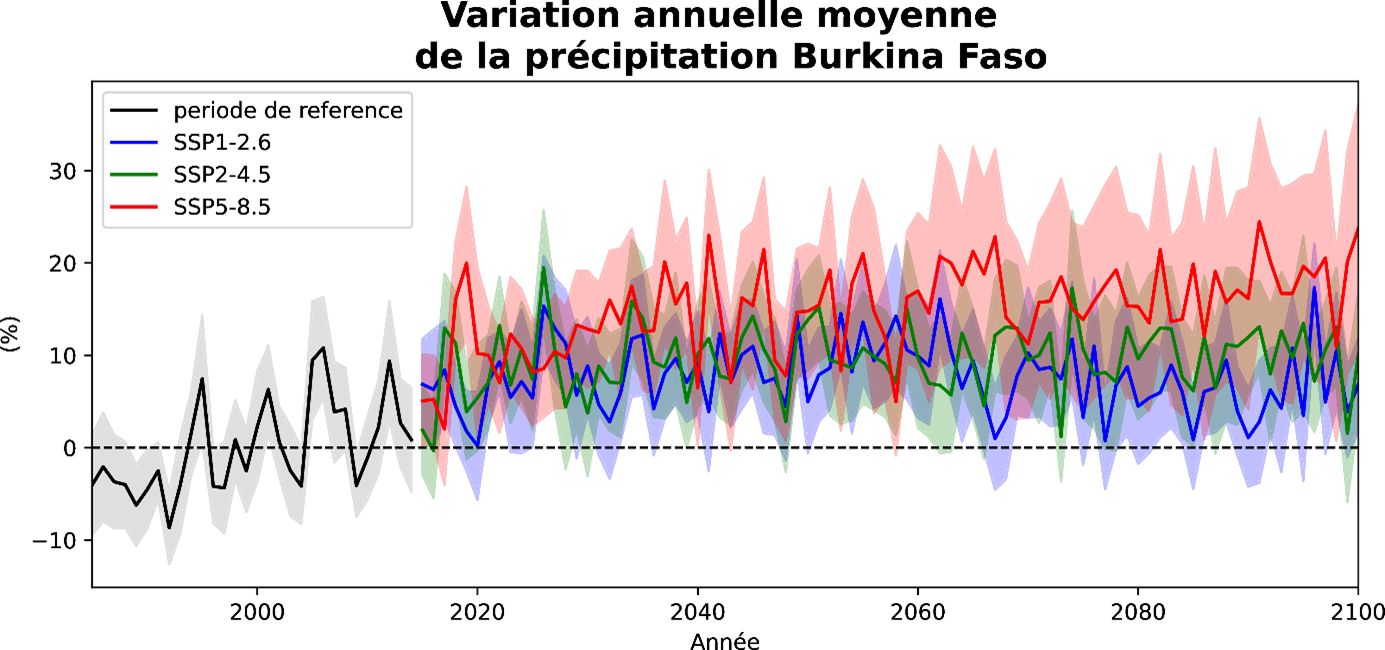
\includegraphics{Figures and Photos/Figure 8.png}
\caption{\textbf{Figure 8: Mean annual change in precipitation in Burkina Faso}}
\end{figure}

\emph{Source: Consultant for the revision of the NAP}

\begin{figure}
\centering
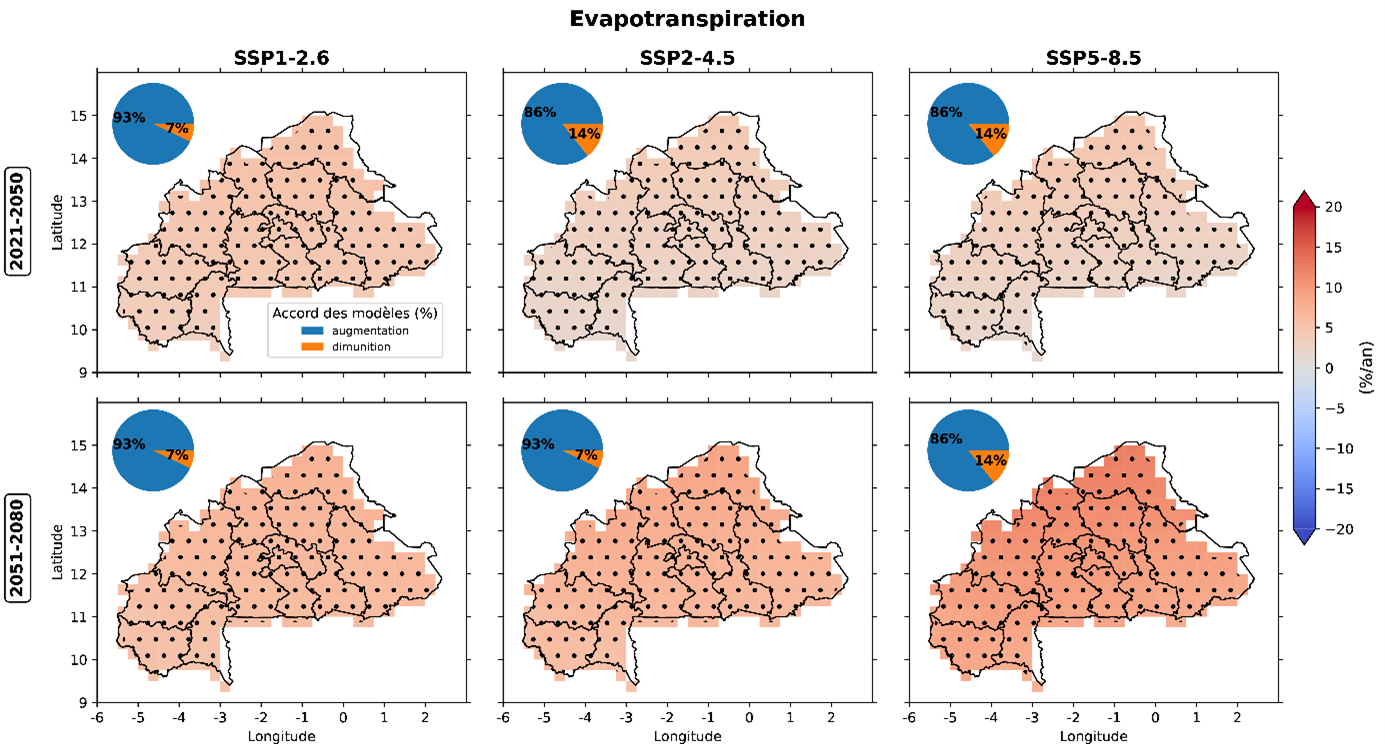
\includegraphics{Figures and Photos/Figure 9.png}
\caption{\textbf{Figure 9: Similar to Figure 8, but for evapotranspiration}}
\end{figure}

\emph{Source: Consultant for the revision of the NAP}

\subsection{Annual Air Temperature}\label{annual-air-temperature}

Air temperatures are expected to rise in Burkina Faso. The overall average of the models predicts a significant increase in air temperature (Figure 10). The temperature rises as climate scenarios change from low to high emissions and towards the end of the century. The western and northern parts of the country will experience greater warming, but the north will have a higher increase. The Sahel, North and Centre-North parts are expected to rise by about 1.0°C (SSP1-2.6), 1.3°C (SSP2-4.5) and 1.5°C (SSP5-8.5) in the near future. 100\% of models project greater warming, exceeding 5°C for the period 2051-2080 according to SSP5-8.5 over the northern part of the country. In the east of the country, the warming of air temperature is expected to be lower compared to other regions.

Figure 11 shows the projection of inter-annual air temperature variability under different scenarios. The overall average predicts warming in Burkina Faso compared to the baseline period. Warming under the SSP5-8.5 scenario is projected to continue to increase beyond 2100. The country is expected to experience a warming of about 5.5°C by the end of the century. The SSP1-2.6 and SPP2-4.5 scenarios have similar patterns, but with different amplitudes. In other words, warming in Burkina Faso could stabilize below both SSPs, with a maximum of 2.0°C and 1.0°C under SSP2-4.5 and SSP1-2.6, respectively. Based on SSP1-2.6, the country is projected to warm by 0.9°C and 1.1°C between 2021-2050 and 2051-2080, respectively (Figure 11). February shows the highest temperature increase for the period 2021-2050 under SSP1-2.6 and SSP2-4.5, while May shows the largest increase for the period 2051-2080 under SSP1-2.6 and SSP5-8.5. Without any mitigation strategy, average temperature increases could reach 2.8°C below SSP5-8.5; May and April were the months with the highest increases over the 2021-2050 and 2051-2070 periods, respectively. In addition, the average air temperature is expected to reach 4.2°C in the distant future and reach 1.5°C in the near future. The models even predict warming during the harmattan period (December-January-February) in all scenarios and periods considered. High temperatures are particularly damaging to crop production when they occur during the flowering period of crops. This indicates that rising air temperatures in Burkina Faso could cause damage to agriculture. In addition, rising temperatures could also reduce the potential for photovoltaic power generation in the country, as solar PV technology is sensitive to rising air temperatures (Sawadogo et al., 2020).

\begin{figure}
\centering
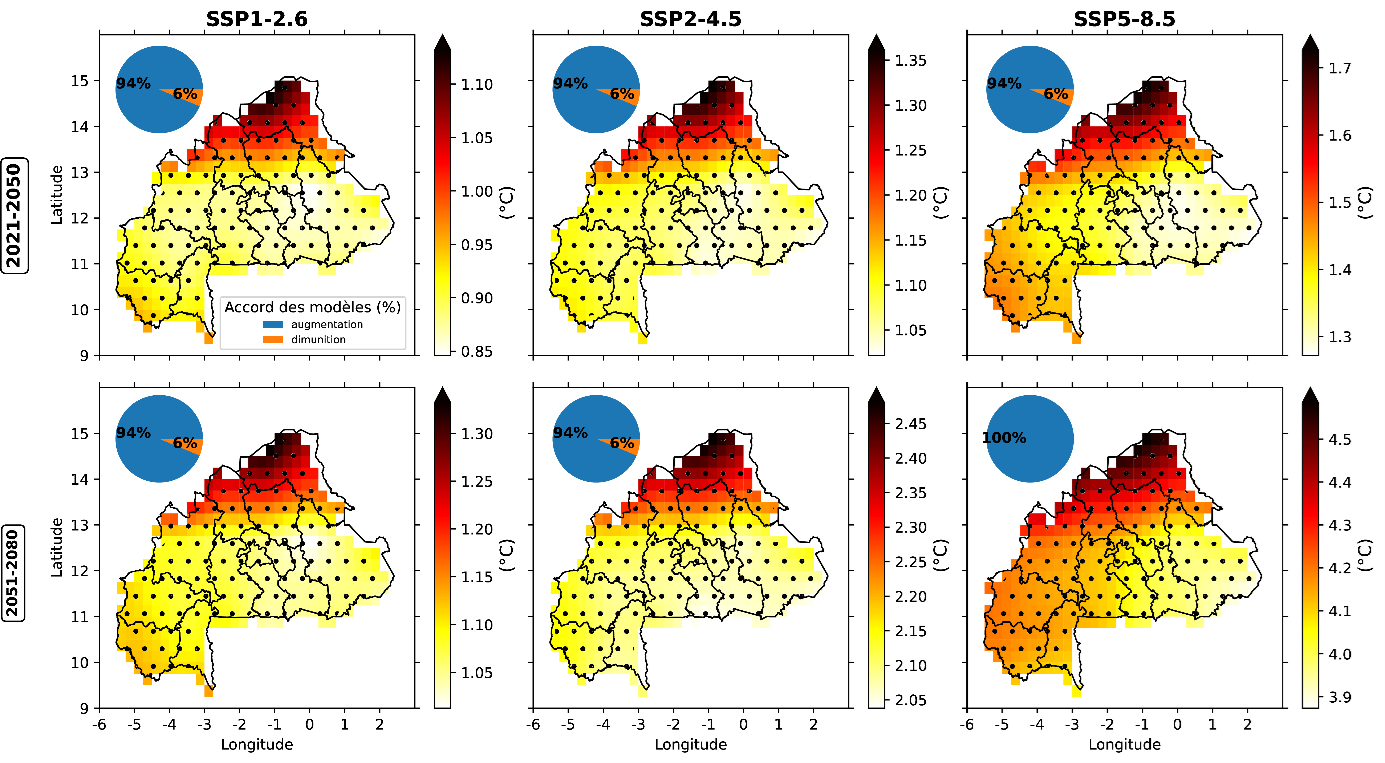
\includegraphics{Figures and Photos/Figure 10.png}
\caption{\textbf{Figure 10: Similar to Figure.9, but for temperature}}
\end{figure}

\emph{Source: Consultant for the revision of the NAP}

\begin{figure}
\centering
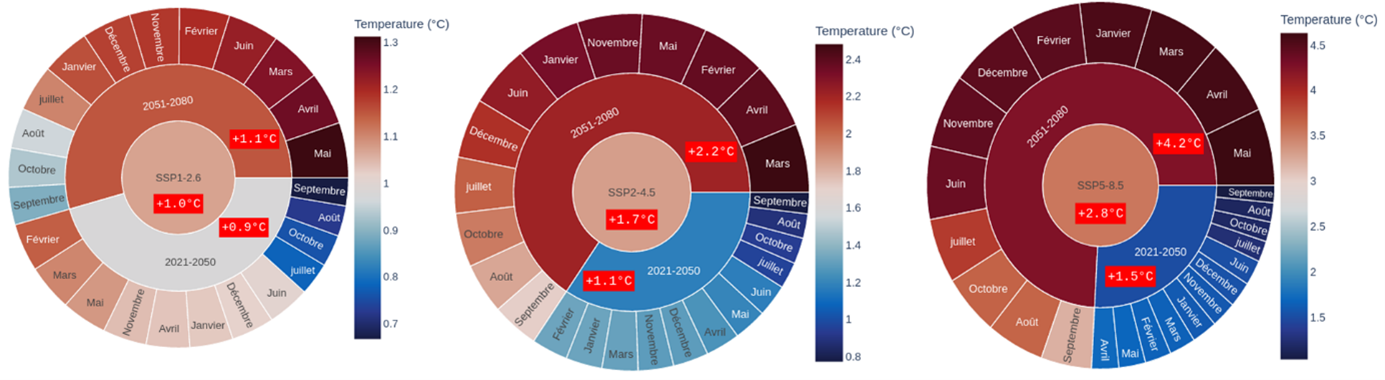
\includegraphics{Figures and Photos/Figure 11.png}
\caption{\textbf{Figure 11: Multi-model average of projected changes in air temperature for each month under the three climate scenarios (SSP1-2.6, SSP2-4.5 and SSP5-8.5) for the near future (2021-2050) and the distant future (2051-2080)}}
\end{figure}

\emph{Source: Consultant for the revision of the NAP}

The red box indicates the average of the SSP time period.

\begin{figure}
\centering
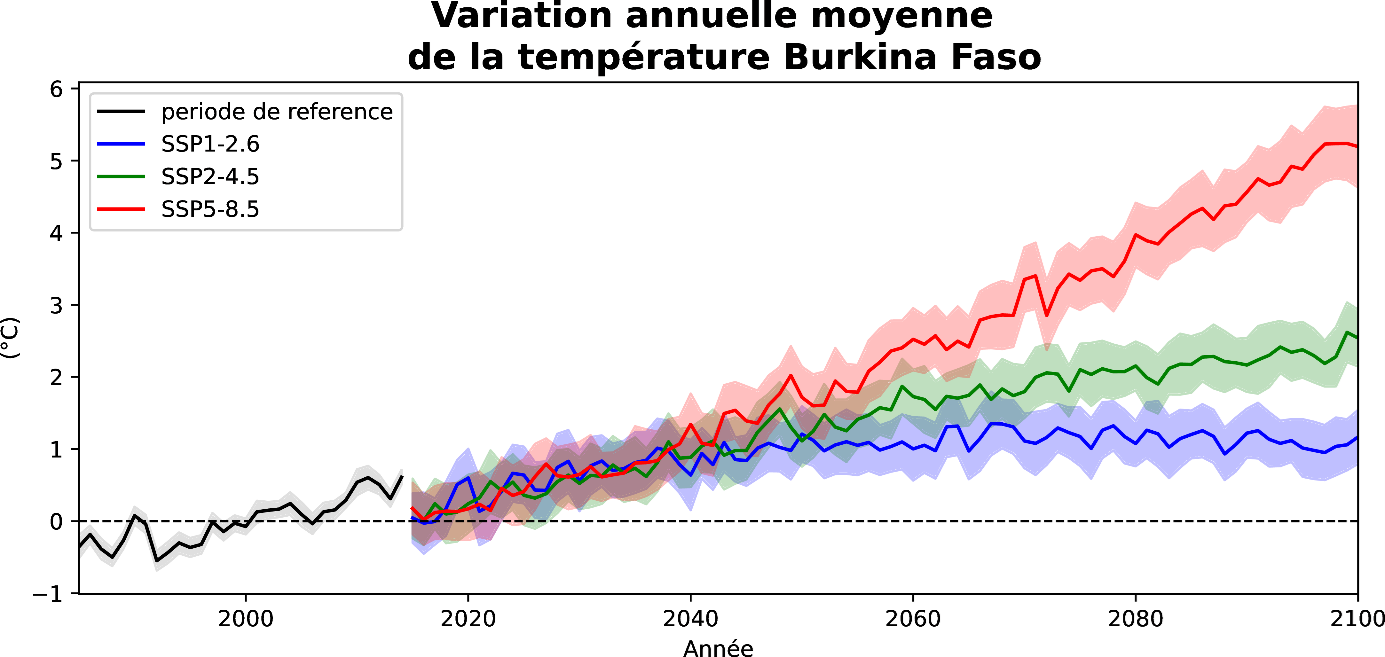
\includegraphics{Figures and Photos/Figure 12.png}
\caption{\textbf{Figure 12: Average annual temperature change in Burkina Faso}}
\end{figure}

\emph{Source: Consultant for the revision of the NAP}

\subsection{Drought Index}\label{drought-index}

To characterize drought, the maximum number of consecutive dry days during the rainy season with daily rainfall of less than 1 mm was used. The increase in this index means that the probability of drought conditions increases (Figure 13). It is expected that the maximum number of consecutive dry days in some parts of the country under SSP2-4.5 and SSP5-8.5 will increase in the distant future. In other words: Drought conditions could occur in the western part of the country. In the central and northern parts of the country, a decrease of about 1 day is expected. However, these changes are not significant, except for SSP2-4.5 for the period 2051-2080. In addition, there is no agreement between the models on the changes in the sign of the maximum dry period in the country as less than 80\% of the models agree on the sign of the change. Uncertainty decreases towards the end of the century, especially with SSP2-4.5 and SSP5-8.5 scenarios. In the SSP5-8.5 scenario, only 65\% of the models agree on a significant decrease in this drought index of about 1 day, expected in the eastern part of the country. These projected changes in this region should be used to formulate climate change adaptation measures. However, the non-significant changes expected in other regions under different scenarios and time periods should not deter policymakers and stakeholders from taking action to reduce the impact of drought events in agriculture. Indeed, these regions are currently experiencing frequent droughts and have a huge impact on cereal production (Africa RiskView, 2020).

\begin{figure}
\centering
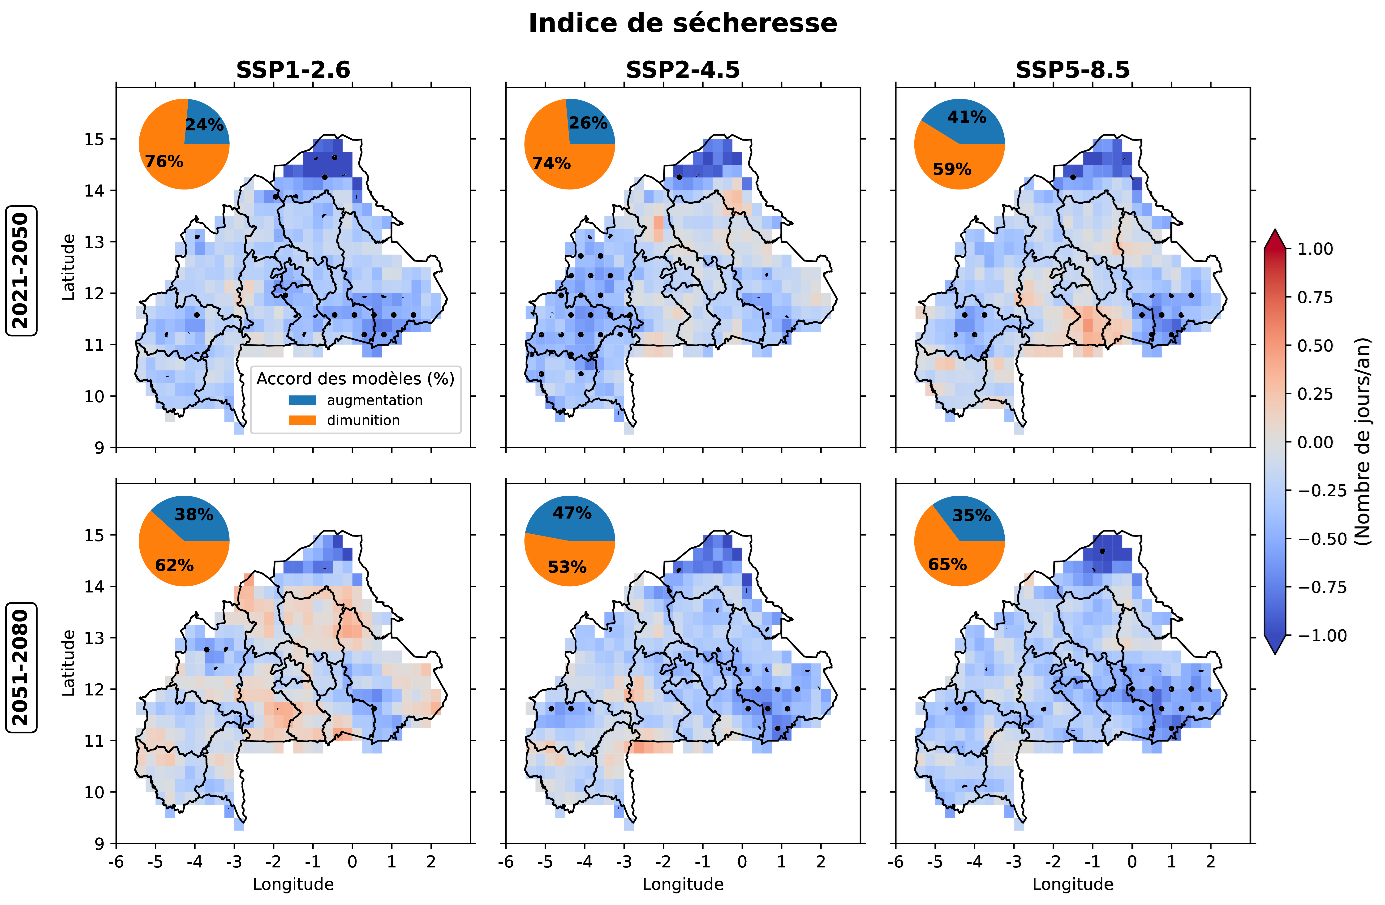
\includegraphics{Figures and Photos/Figure 13.png}
\caption{\textbf{Figure 13: Similar to Figure 10, but for the drought index}}
\end{figure}

\emph{Source: Consultant for the revision of the NAP}

\subsection{Extreme Flooding and Rainfall}\label{extreme-flooding-and-rainfall}

The flood index used here is defined as the maximum amount of precipitation over five days in a given period. This is a measure of heavy precipitation, with high values indicating a high probability of flooding. An increase in this index over time means that the risk of flooding will increase. The overall average of the models predicts an increase in the flood index in Burkina Faso (Figure 14). All models agree on the sign of a significant increase in flood risk in all regions of the country. The magnitude of change increases as the climate change scenario moves towards the highest emissions scenario. In other words, the risk of flooding is more pronounced in the SSP5-8.5 scenario than in the SSP1-2.6 scenario. In addition, the increase is more intense in the distant future than in the near future. The risk of flooding is expected to increase by more than 20\% in the country, especially in the period 2051-2080. The north and east of the country are expected to see a larger increase. Under the SSP1-2.6 scenario, the risk of flooding could increase by 5\% per year in the near future, while it doubles in the distant future.

Another climate index was also used to determine the number of days per period with daily precipitation of at least 20 mm. This climate index is a measure of extreme precipitation, with high values associated with a high probability of flooding. An increase in this index over time means that the risk of flooding will increase. As with the 5 consecutive rainy days, the number of rainfall events greater than 20 mm/year will increase in the country (Figure 15). More than 80\% of the models agree on the sign of change and they are all statically significant at a 95\% confidence level. The occurrence of heavy precipitation events also increases when the level scenario increases and the frequency of the number of days in the distant future are high. The SSP5-8.5 scenario shows the largest increase for the different periods considered. The number of days is expected to increase by more than 4 days. Flooding may be more frequent in the eastern part of the country. The increased risk of flooding could displace many people and important infrastructure could be damaged. Increased flood risk could also lead to an increase in waterborne diseases and threaten health systems due to stagnant waters, flooding of water supplies, and disruption of water supply and sanitation systems. In addition, flood risk can also contribute to reduced crop yields, loss of beneficial soil invertebrates, including earthworms, and increased risk of animal diseases such as liver fluke infestation.

\begin{figure}
\centering
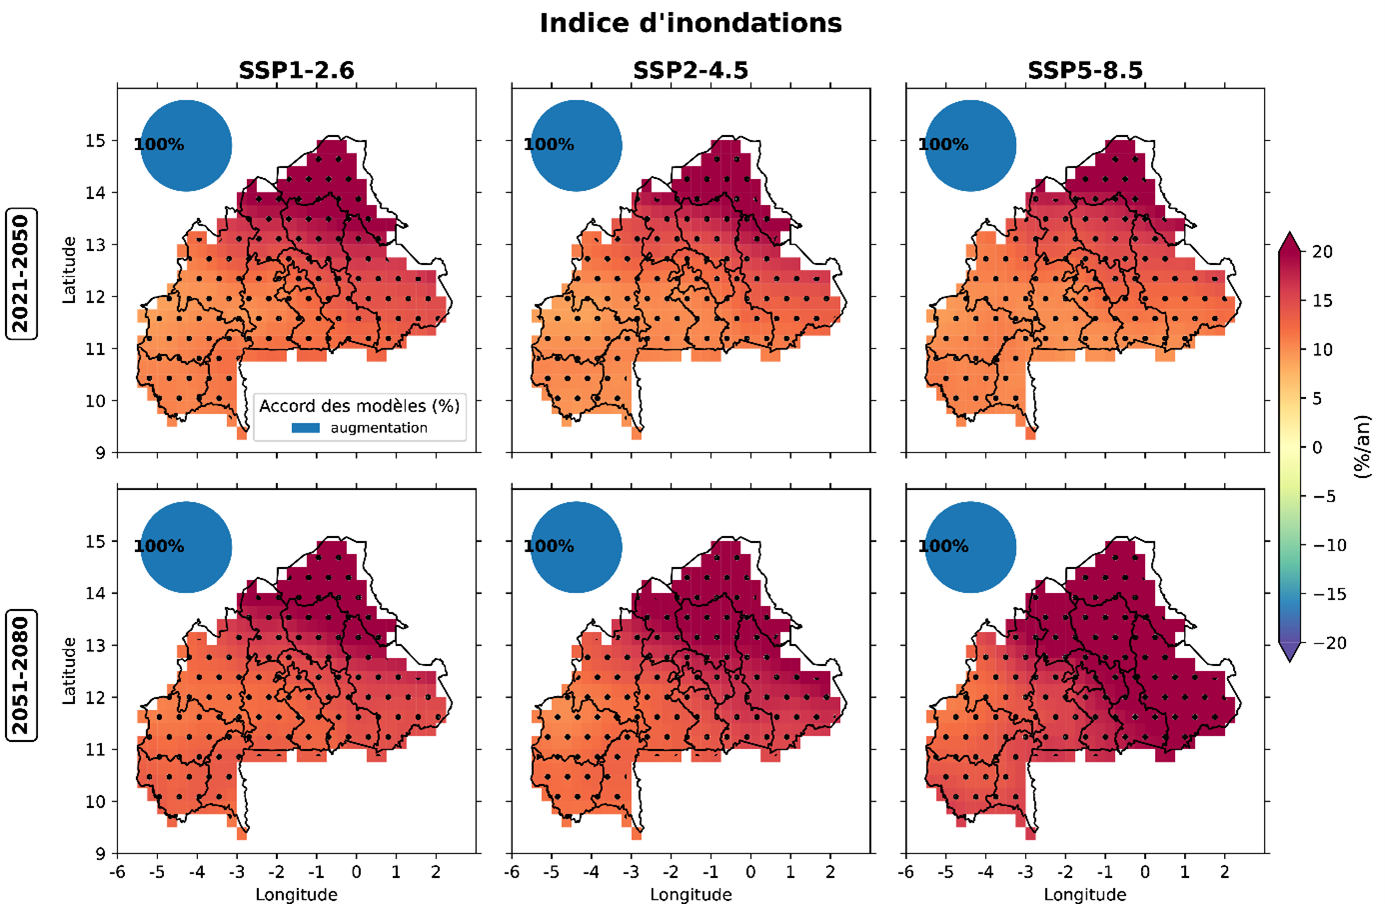
\includegraphics{Figures and Photos/Figure 14.png}
\caption{\textbf{Figure 14: Similar to Figure 13, but for the flood index}}
\end{figure}

\emph{Source: Consultant for the revision of the NAP}

\begin{figure}
\centering
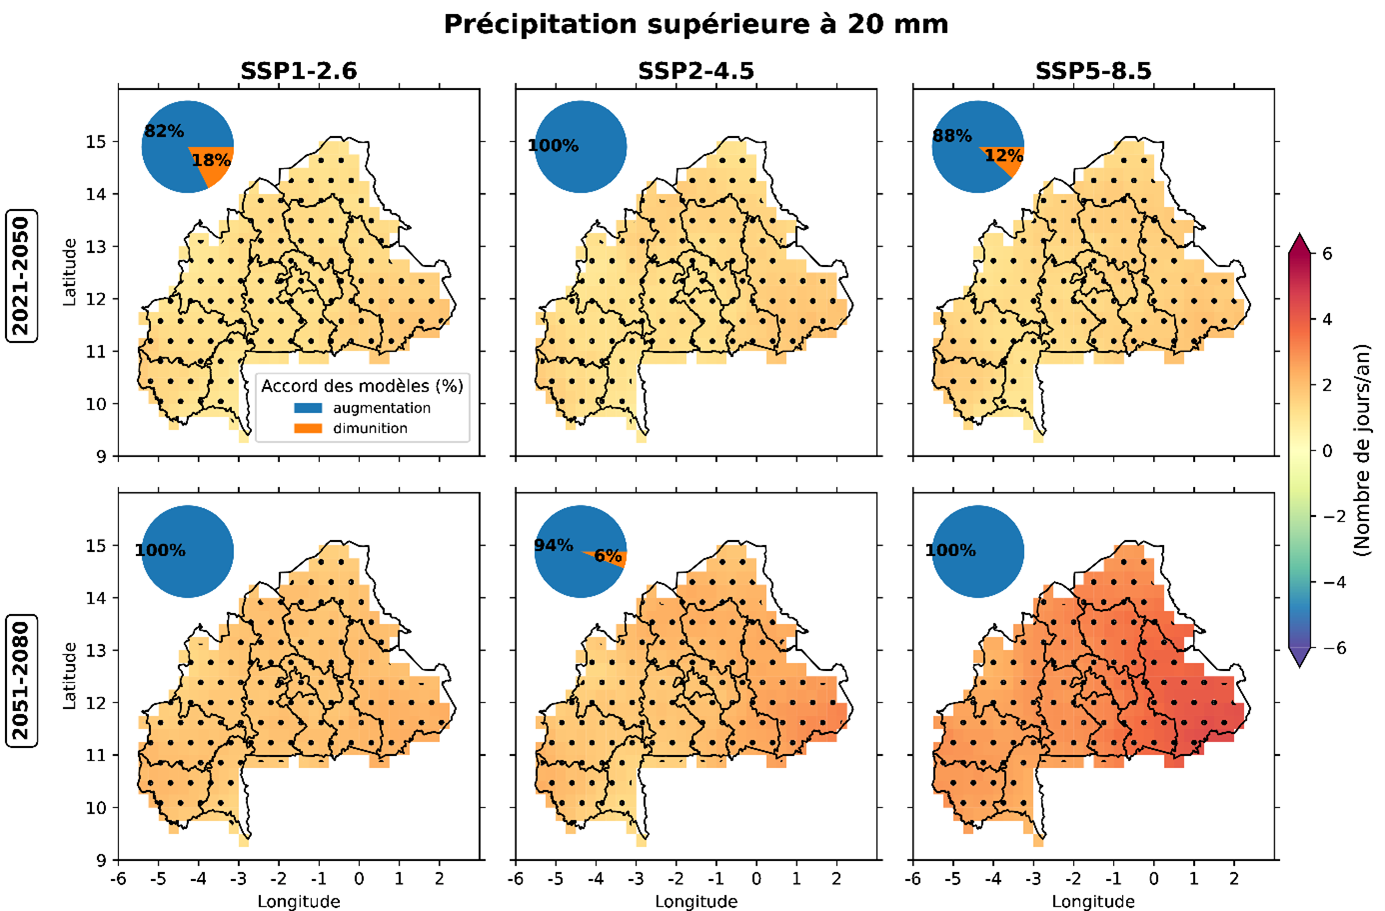
\includegraphics{Figures and Photos/Figure 15.png}
\caption{\textbf{Figure 15: Similar to Figure 14, but for precipitation greater than 20 mm}}
\end{figure}

\emph{Source: Consultant for the revision of the NAP}

\subsection{Heat Index}\label{heat-index}

All models agree on the projected change in heat stress days in Burkina Faso (Figure 16). Heat stress days above 41°C are likely to increase in Burkina Faso. The number of days varies depending on the scenario and time period. SSP1-2.6 shows the smallest increase (up to 30 days), while SSP5-8.5 shows the largest increase (up to 80 days) for the period 2021-2050. The increase in the number of heat stress days is most pronounced for the period 2051-2080. In the northern part of the country, the increase will be small compared to other regions in all scenarios and periods because the relative humidity in this area is low. However, more people will suffer from heat cramps and exhaustion, especially in the western part of the country. Under the SSP5-8.5 scenario, an increase of about 160 days of heat stress per year is projected by the end of the century.

\begin{figure}
\centering
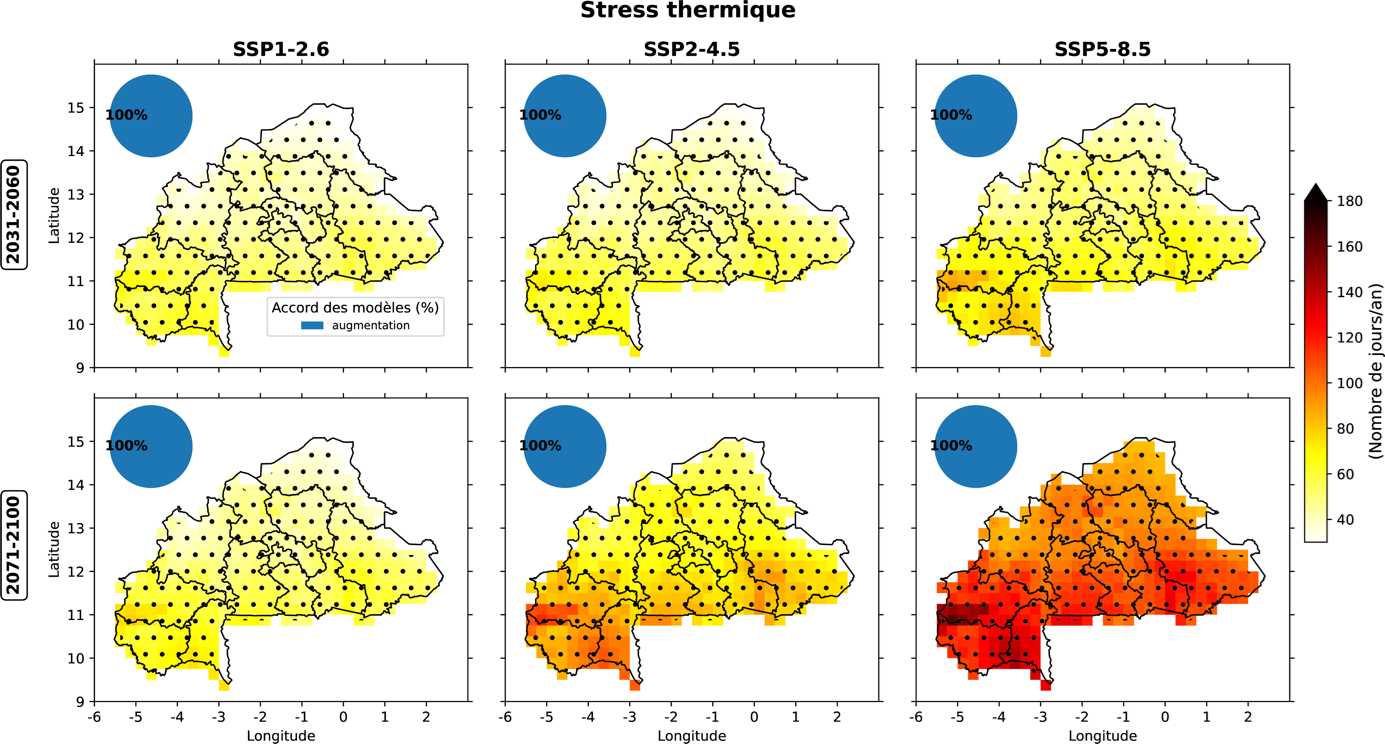
\includegraphics{Figures and Photos/Figure 16.png}
\caption{\textbf{Figure 16: Similar to Figure 15, but for heat stress}}
\end{figure}

\emph{Source: Consultant for the revision of the NAP}

To quantify the temporal distribution of heat stress throughout the year, Figure 17 shows the number of heat stress days above 41°C per month. This figure is obtained by averaging all grid points in the Burkina Faso domain with the overall average of the models. The overall average predicts an increase in heat stress days throughout the year for all scenarios and periods. In both time periods, the SSP5-8.5 scenario has the highest number of heat stress days. The number of heat-stressed days may increase in March and July for all three climate scenarios and the period considered, but more intensively in the period 2051-2080. Approximately 14 days in March and 11 days in June may exhibit more heat stress under the SSP5-8.5 scenario in the distant future. For the period 2021-2080, March, April, June, July, and November show a slightly similar increase in the number of days in all scenarios (\textasciitilde6 days). The smallest increase may occur in September and October (\textasciitilde1 day) in the near future, while in the distant future the months of October and January could be likely to increase by more than 3 days.

\begin{figure}
\centering
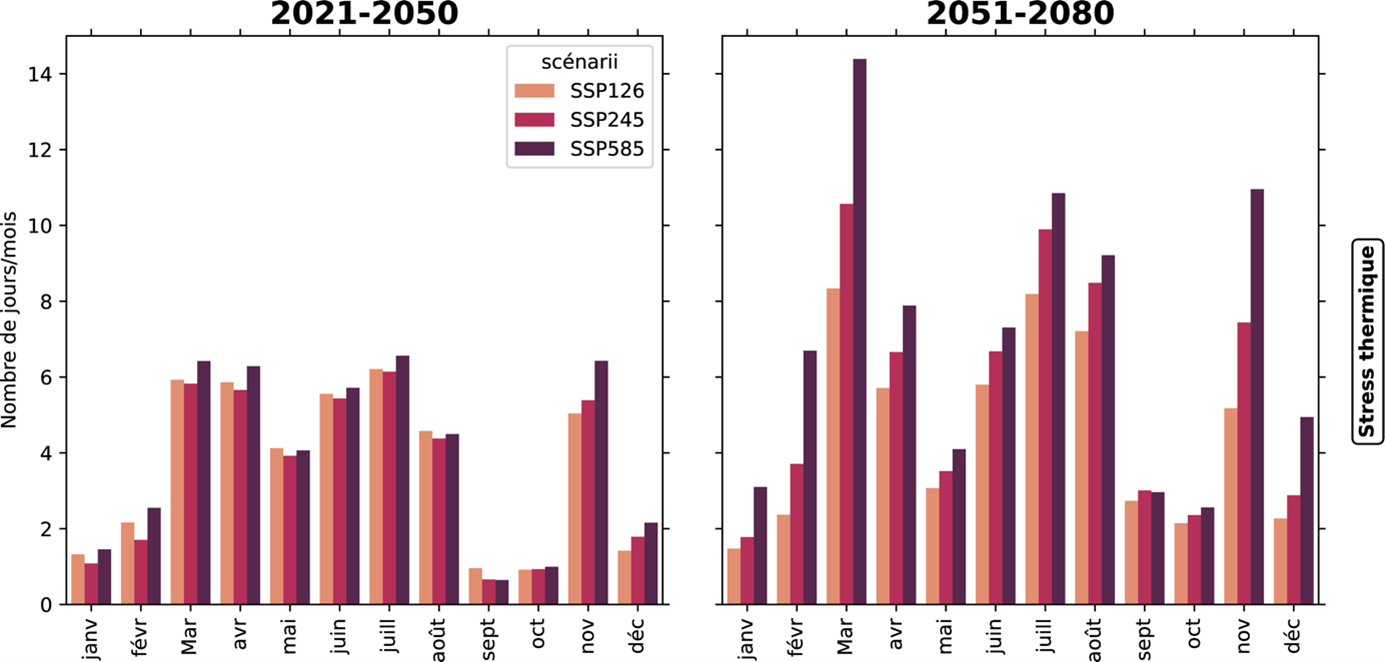
\includegraphics{Figures and Photos/Figure 17.png}
\caption{\textbf{Figure 17: Bar graph of heat stress for different months under different climate change scenarios and for the near future (2021-2050) and the distant future (2051-2080)}}
\end{figure}

\emph{Source: Consultant for the revision of the NAP}

The increase in hot days could also increase health risks for the population and reduce work capacity. Cognitive fatigue and difficulty concentrating, which reduce work efficiency due to increased temperature, can lead to productivity losses (Maula et al., 2016). In addition, at high relative humidity levels, the body stops evaporating water, which prevents the cooling effect of the body and leads to heat illness. Recurrent symptoms such as heat exhaustion are likely. Heat stroke is likely with prolonged exposure and/or physical activity. Older adults (\textgreater{} 65 years of age) may be at higher risk. In summary, Burkina Faso should expect an increase in heat stress days, regardless of the climate change scenario. The western part is known as the economic lung of the country; the expected significant increase in the number of heat stress days could affect the socio-economic activities of the region and thus reduce the country's GDP. There are steps and strategies that need to be taken to accommodate the future increase in heat stress days.

\subsection{Cooling Degree Days}\label{cooling-degree-days}

To characterize the energy demand for cooling a building as a function of climate change, cooling degree days are typically used. A degree-day is defined as the difference between the average daily temperature and a given reference temperature. The most common reference temperature for cooling is around 22°C (Shi et al., 2016). However, this threshold varies according to socio-economic activities, building characteristics and climatic conditions. In Burkina Faso, we assume that thermal comfort is below 30°C. Therefore, cooling degree days are calculated when the temperature of the cooling degree days exceeds 30°C. In other words: we need to cool a building when this value is reached.

All models agree on the sign of a significant increase in cooling degree days in Burkina Faso (Figure 18). The number of days per year increases with the level of the scenario and accelerates towards the end of the century. The number of days is higher in the SSP5-8.5 scenario. The number of days per year exceeds 150 for the period 2051-2080. In the SSP1-2.6 scenario, the number of days could reach about 25 days per year for the period 2021-2050, while it could double for the period 2051-2080. As with heat stress days, some areas in the west of the country could see the largest increase. October shows the largest increase in cooling degree days, while April shows the smallest increase under the SSP5-8.5 scenario for the near and distant future (Figure 19). In March and April, during the hot season, the country already has a high value of cooling degree days; With climate change, the country could experience more months when we need air conditioning for cooling. Global warming could significantly increase the energy consumption of buildings in Burkina Faso, where the country has a low energy security index (IRENA, 2021). Appropriate measures need to be taken by considering the future impact of climate on the characteristics of buildings in the country and by producing more energy, mainly from renewable sources, for cooling buildings.

\begin{figure}
\centering
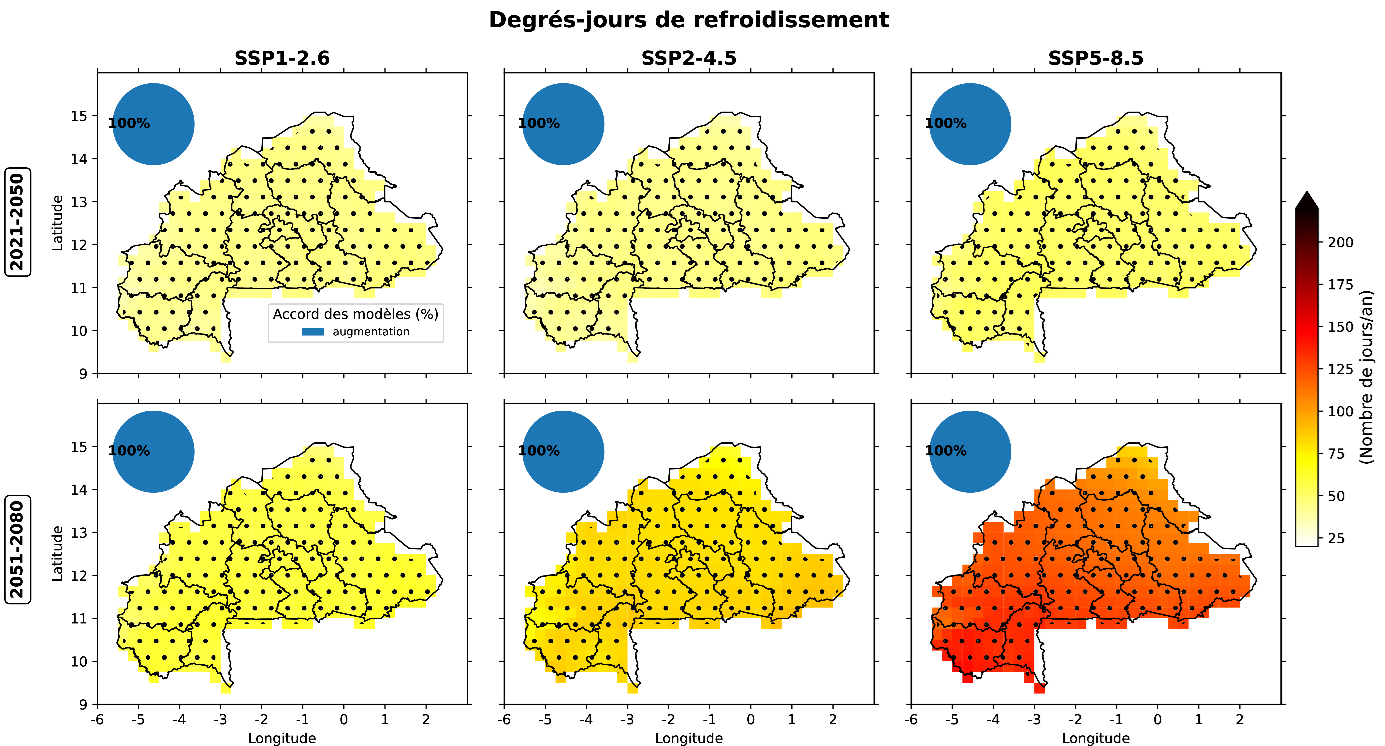
\includegraphics{Figures and Photos/Figure 18.png}
\caption{\textbf{Figure 18: Similar to Figure 16, but for cooling degree days}}
\end{figure}

\emph{Source: Consultant for the revision of the NAP}

\begin{figure}
\centering
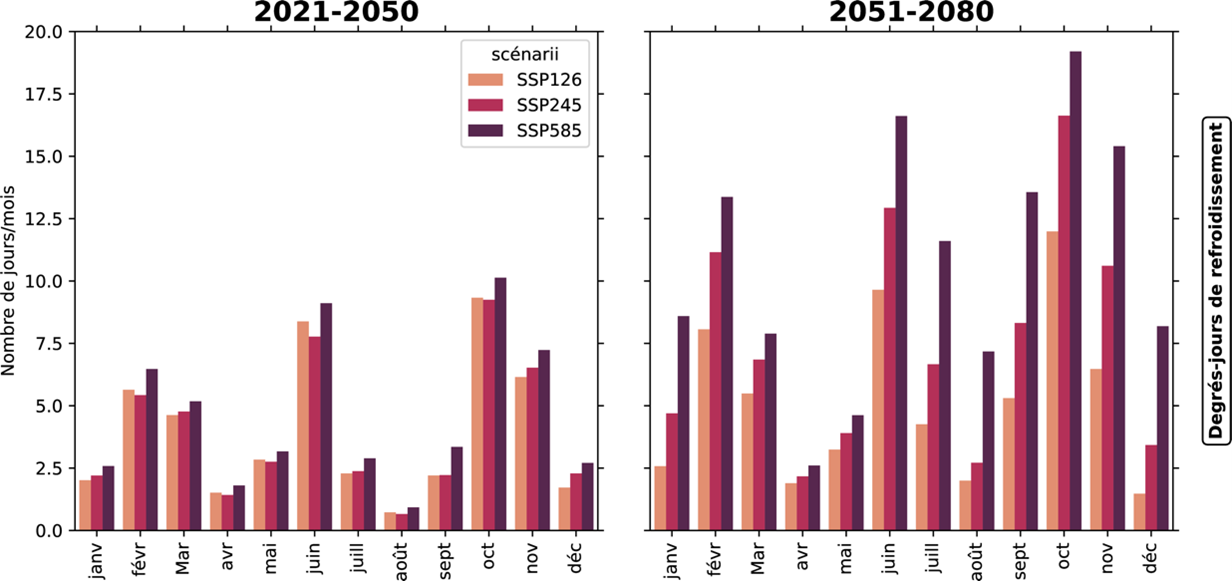
\includegraphics{Figures and Photos/Figure 19.png}
\caption{\textbf{Figure 19: Similar to Figure 17, but for cooling degree days}}
\end{figure}

\emph{Source: Consultant for the revision of the NAP}

\subsection{Population exposure to climate change}\label{population-exposure-to-climate-change}

To better understand the exposure of the population to the impacts of climate change, the total change in exposure (in person events) of the approach developed by Jones et al.~(2015) was used. The total change in exposure is defined here as the exposure of the population to the flood risk index, drought and heat stress. It is calculated by taking the average of all grid points in the Burkina Faso zone, the different climate impact factors and population data. The population data were developed by the International Institute for Applied Systems Analysis (IIASA) and the National Center for Atmospheric Research (CNRA) and are consistent with the SSP scenarios. The spatial resolution of the data is approximately 1 km and the temporal resolution ranges from 2010 to 2100 for the different SSPs (SSP1, SSP2, SSP3, SSP4 and SSP5) in 10-year increments. Historical population data are from Protocol 2b of the Inter-Comparison of Intersectoral Impact Models (ISIMIP2b) project, which serves as the base year (2010). As the PHS population data are presented in 10-year increments, the period 2020-2050 is considered the near future and the period 2050-2080 is considered the far future. Table 3 summarizes the matrix with the PHC definitions for the demographic and human capital components for the high-fertility country. From this table, it is clear that SSP2 scenarios show the highest population growth.

\begin{tabular}{>{\raggedright\arraybackslash}p{15em}|>{\raggedright\arraybackslash}p{15em}|>{\raggedright\arraybackslash}p{15em}|>{\raggedright\arraybackslash}p{15em}|>{\raggedright\arraybackslash}p{15em}}
\hline
\multicolumn{5}{c}{Table 3: Matrix with SSP definitions for demographic and human capital components for the high-fertility country} \\
\cline{1-5}
Scenario & Fertility & Mortality & Migration & Education\\
\hline
SSP1 & Weak & Weak & Medium & Strong\\
\hline
SSP2 & Medium & Medium & Medium & Medium\\
\hline
SSP5 & Weak & Weak & Strong & Strong\\
\hline
\end{tabular}

\emph{Source: KC and Lutz, 2017}

Approximately two (2) million people in Burkina Faso may be affected by floods in the coming years according to SSP1-2.6 and SSP5-8.5 scenarios (Figure 20a). This number could increase in the SSP2-4.5 scenario. In addition, approximately 4 million people could be exposed to heat stress in the near future in SSP1-2.6 and SSP5-8.5 scenarios (Figure 20b). Under scenario SPP2-4.5, the number of populations likely to be affected could increase by about 4.5 million in the period 2021-2050 and by 7.5 million in the period 2051-2080. This could put a strain on health systems and lead to an increase in heat-related deaths due to rising temperatures. About 70\% of Burkina Faso's population depends on rainfed agriculture for their livelihoods (Sorghum et al., 2021), meaning that any increase in the drought index could lead to widespread food insecurity.

SSP2-4.5 models predict that approximately 250,000 people will be affected by projected changes in the drought index in both the short and long term (see Figure 20b). Conversely, SSP1-2.6 and SSP5-8.5 scenarios show more impacts on the drought index in the long term (200,000 people) than in the short term (150,000 people).

\begin{figure}
\centering
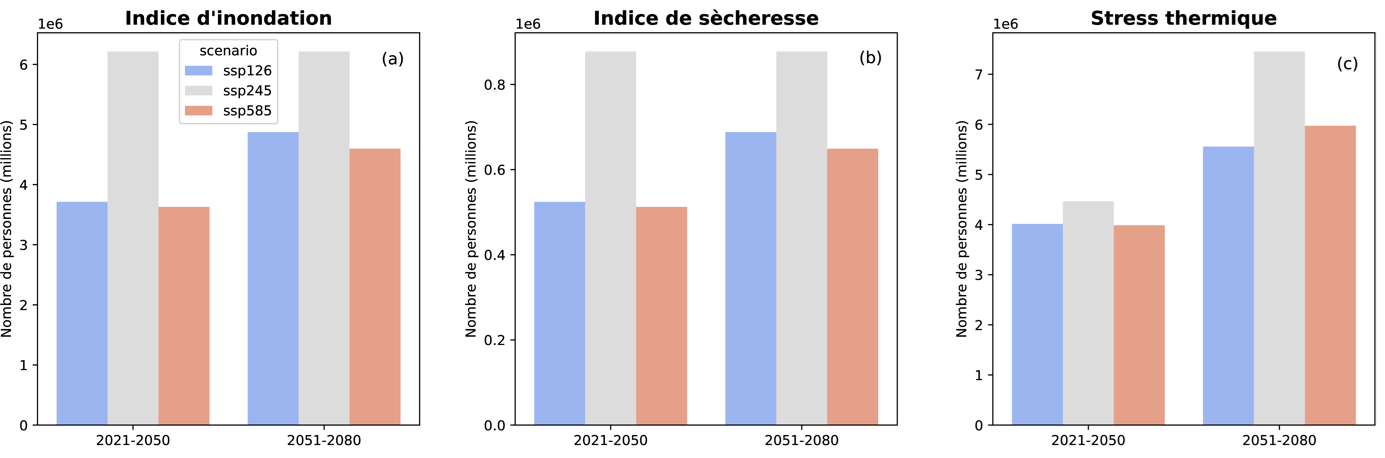
\includegraphics{Figures and Photos/Figure 20.png}
\caption{\textbf{Figure 20: Projection of the total change in the population's exposure to: (a) flood risk (unit, event per person per day), (b) drought (unit, event per person per day) and (c) heat stress (unit, event per person per day) according to different climate scenarios and time periods}}
\end{figure}

\emph{Source: Consultant for the revision of the NAP}

Figure 21 summarizes all the projections averaged for Burkina Faso for different climate change scenarios and time periods. The average of all models agrees on most projected climate impacts, with the exception of the onset of rainfall and the drought index. The overall average of the models predicts a significant increase in most climate impact factors in Burkina Faso. The country is facing many impacts of climate change, and given these climate projections, the country will be even more vulnerable if adaptation strategies are not implemented. The value of each cell indicates the actionable changes. The red down arrow indicates a decrease in change, the yellow right arrow indicates no change, and the up arrow shows an increase in change. The symbol with the red cross indicates that the models do not match, while the checkmark indicates that more than 80\% of the models agree on the sign of the changes.

For the prioritization of adaptation measures, the climate risk factors in the context of this NAP are grouped into three major climate risks, namely drought, floods and extreme heat (see Table 4).

\begin{figure}
\centering
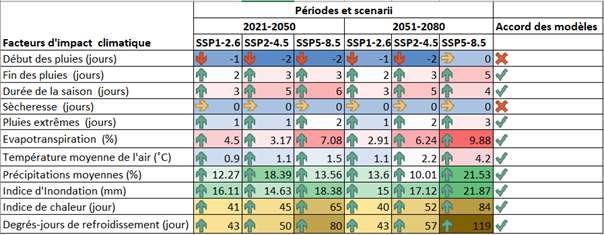
\includegraphics{Figures and Photos/Figure 21.png}
\caption{\textbf{Figure 21: Projection of the different climatic factors averaged over Burkina Faso under different scenarios and periods}}
\end{figure}

\emph{Source: Consultant for the revision of the NAP}

\textbf{Table 4: Climate risks considered in the NAP and associated impact factors}

\begin{tabular}{>{\raggedright\arraybackslash}p{12em}|l}
\hline
\multicolumn{2}{c}{Table 4: Climate risks considered in the NAP and associated impact factors} \\
\cline{1-2}
Climate risk & Factors of climate impacts\\
\hline
Flooding & Flood Index\\
\hline
 & Extreme Rainfall\\
\hline
Drought & Beginning of the rains\\
\hline
 & End of the rains\\
\hline
 & Length of the season\\
\hline
 & Evapotranspiration\\
\hline
High temperatures & Heat Index\\
\hline
 & Cooling Degree Days\\
\hline
\end{tabular}

\emph{Source: Burkina Faso Climate Vulnerability Study Report}

\section{Identification of climate impacts and risks and assessment of vulnerabilities of development sectors to climate change}\label{identification-of-climate-impacts-and-risks-and-assessment-of-vulnerabilities-of-development-sectors-to-climate-change}

In Burkina Faso, all the development sectors included in the NAP have vulnerability factors to the adverse effects of climate change. The major risks in order of importance are droughts, floods, extreme heat, etc.

A portrait of climate-related impacts, vulnerabilities and risks in the sectors selected for this NAP is summarized in the table below.

\textbf{Table 5: Synthesis of impacts, vulnerabilities and risks for NAP sectors}

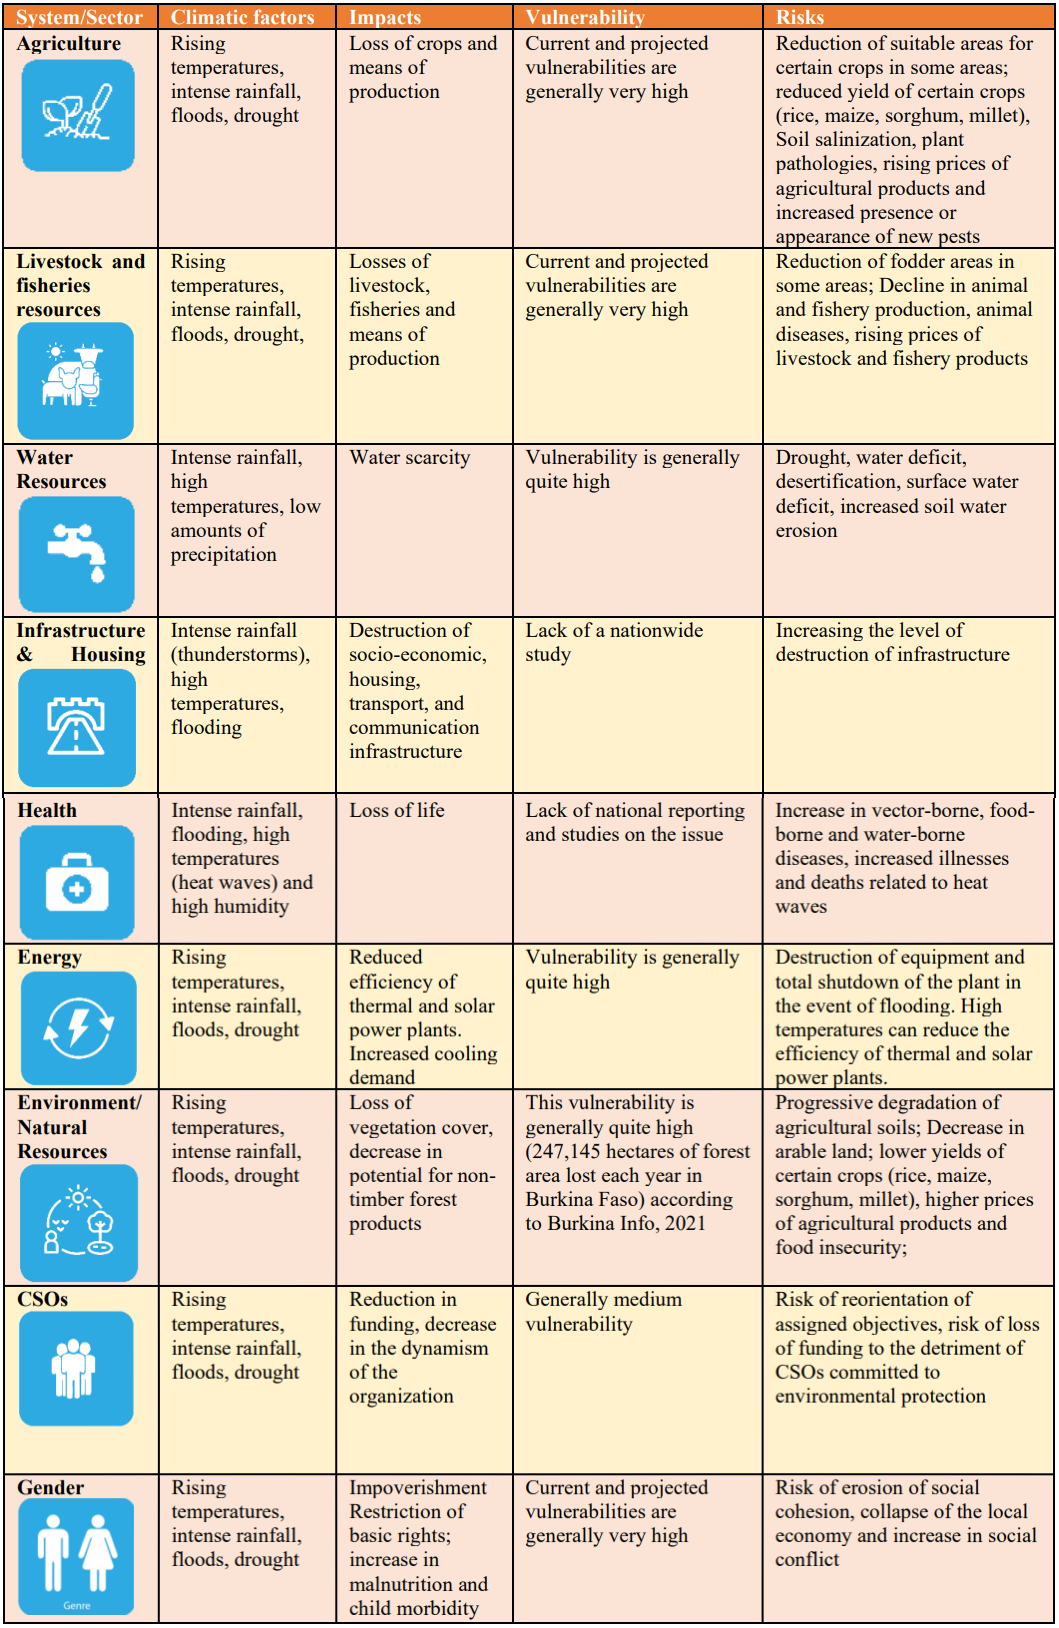
\includegraphics{Tables/Table 5.PNG}

\emph{Source: Burkina Faso Climate Vulnerability Study Report}

\chapter{NAP implementation planning and strategy}\label{nap-implementation-planning-and-strategy}

\section{NAP guiding principles}\label{nap-guiding-principles}

The formulation of Burkina Faso's National Climate Change Adaptation Plan (NAP) was made with reference to the guidance of the Least Developed Countries Expert Group, carried out in accordance with decision 1/CP.16. The formulation, implementation and monitoring and evaluation of the NAP is based on principles whose choice has been guided by its adequacy with those mentioned in the UNFCCC framework document and those mentioned in certain strategic policy and orientation documents at the national level, in particular the National Prospective Study, the second National Economic and Social Development Plan (PNDES II), the Action Plan for the Stabilization and Development of the Transition (PA-SDT) and the National Sustainable Development Policy (PNDD).

These guiding principles are listed as follows:

\begin{itemize}
\item
  \textbf{Participation:} Climate change knows no sectoral boundaries, let alone administrative boundaries. Given their scope, it is therefore important to seek the involvement of all development actors at different scales, from the identification of adaptation actions to their implementation. The successful implementation of the NAP requires the availability and access of stakeholders to scientific and technical information and data is very essential to guide practical intervention choices. The opinions and priorities of the beneficiaries will be taken into account in the process of operationalizing the options and adaptation measures recommended in accordance with the regulations in force;
\item
  \textbf{Coherence of interventions:} This principle implies that actions must be carried out in a coherent and concerted manner with a view to obtaining more convincing results. The transversality of climate change implies actions in several sectors and mobilizing both public and private actors. Thus, siloed actions can have unintended adverse consequences. In order to avoid such a situation, the search for synergy, the establishment of public-private partnerships and a ``system'' approach must be at the heart of the definition and implementation of adaptation actions. Coherence is therefore essential in the implementation of the NAP to ensure that it complies with and corresponds to the development priorities defined at the national level but also to the modalities of effective intervention required;
\item
  \textbf{Empowerment of stakeholders:} Empowerment of stakeholders is an essential step in achieving results. It is the result of the participatory approach. In order to ensure effectiveness and efficiency in achieving the objectives assigned to the NAP, the effective involvement of all actors in preparing and leading actions leading to change is essential. The essential characteristic of accountability is to involve and engage the actors involved in the implementation of the strategy in relevant actions likely to bring about changes in behaviour;
\item
  \textbf{Decentralization of actions:} Since 2004, Burkina Faso has implemented decentralization, which implies that development must also be thought of and managed at a lower level, the commune. As a result, development must be based on local potential, which is largely dependent on natural resources that are highly sensitive to local change. Thus, the issue of adaptation to climate change must now be taken into account in the elaboration and implementation of local development policies so that development efforts are not in vain. Local authorities will identify the adaptation options to be taken to counter the effects of climate change within their territorial boundaries and will take charge of them through Regional and Communal Adaptation Plans;
\item
  \textbf{Taking into account gender and inclusion:} The adaptation options identified in the NAP require the participation of men and women in actions for greater relevance and significant impacts. Therefore, in view of the increased vulnerability of women to the adverse effects of climate change and their participation in development, an approach based on partnership, the promotion of social dialogue, the reduction of inequalities, the development of the adaptive capacities of all social strata, especially the most vulnerable, and the pre-eminence of good governance is necessary;
\item
  \textbf{Equity:} The search for equity, particularly social and environmental equity, in the implementation of the NAP must be required to ensure the coherence and continuity of the sustainability of interventions. This principle guarantees the reduction of social and regional inequalities and national solidarity, which will be the determining thread to ensure intra- and inter-generational equity, gender consideration, as well as the consideration of the specificities of regions and localities by enhancing their potential, for more spatial equity, more social cohesion and peace;
\item
  \textbf{Partnership and subsidiarity:} There is a need for a permanent dialogue between representatives of the different groups of actors in a given development sector. The partnership will enable the synergy and co-financing of the NAP's actions. The partnership will have to take the form of the judicious involvement of local government and private sector actors through the strengthening of the Public-Private Partnership (PPP), civil society and TFPs in the implementation of the actions chosen. Isolated and sectoral interventions have indeed shown their inadequacies in the search for coherence and effectiveness;
\item
  \textbf{Results-Based Management:} The application of results-based management (RBM) is more than beneficial, especially as it improves efficiency and accountability practices in the planning, implementation, monitoring and evaluation of public policies, with a focus on the achievement of realistically defined results. In addition, transparency and accountability, which are fundamental elements of RBM, are essential for achieving development results, as they help to build trust and ensure the full participation of actors in the achievement of the defined objectives. Burkina Faso has an MRV framework and this NAP is part of this dynamic;
\item
  \textbf{Sustainability:} The sustainability of the NAP's actions implies the rational use of ``natural'' resources, taking into account the needs of current generations without compromising those of future generations. Sustainability takes into account economic, social, environmental and cultural constraints and promotes responsible production and consumption patterns, solidarity, precaution, participation and responsible commitment.
\item
  \textbf{Proactivity and economic intelligence:} The implementation of the NAP must be part of a forward-looking approach, at the level of all actors, in order to face threats of all kinds and to exploit the best opportunities offered, in the short, medium and long term. Proactivity, in the current context of the security challenge, presupposes that all development actors must act with a view to preventing and consolidating security. From then on, proactivity will be based on Economic Intelligence (EI) as a mode of governance based on the monitoring, exploitation and protection of strategic information, the control of risks (security, economic, etc.) and influence on the national and international environment.
\end{itemize}

\section{Vision and strategic directions}\label{vision-and-strategic-directions}

\subsection{Vision of the NAP}\label{vision-of-the-nap}

In addition to these guiding principles, in order to better guide the actions to be implemented within the framework of the NAP, the following vision was formulated: \textbf{``Burkina Faso manages its economic and social development more effectively through the implementation of planning mechanisms and measures that take into account resilience and adaptation to climate change by 2050''}.

\subsection{Objectives}\label{objectives}

Burkina Faso's NAP aligns with the UNFCCC guidelines, which set the following overall objectives:

\begin{itemize}
\item
  reduce vulnerability to the impacts of climate change by building adaptive and resilience capacities;
\item
  facilitate the integration of climate change adaptation, in a coherent manner, into new or existing policies, programmes or activities, into specific development planning processes and strategies within relevant sectors and at different levels.
\end{itemize}

Based on these global objectives of the convention, Burkina Faso's NAP has set objectives for long-term climate adaptation.

These objectives are in line with the global goal on adaptation and those of the current national development frameworks, in particular the National Prospective Survey, the PNDES II and the PA-SDT. As a reminder, the global goal aims to guide efforts and improve adaptive capacity, as well as build resilience and reduce vulnerability to climate change.

\textbf{➢ Overall Objective}

The overall objective of the NAP is to strengthen the resilience of people and ecosystems to climate change for inclusive and sustainable growth in Burkina Faso.

\textbf{➢ Specific Objectives}

Specifically, the NAP aims to:

\begin{itemize}
\item
  strengthen the adaptive capacities of people and ecosystems;
\item
  ensure the systematic integration of climate change adaptation into planning and budgeting at the national and local levels;
\item
  improving the mobilization of climate change adaptation finance;
\item
  promote research and development, local knowledge, know-how and endogenous best practices related to climate resilience, taking into account gender equality;
\item
  improving the governance of climate change adaptation.
\end{itemize}

\section{Adaptation options by sector}\label{adaptation-options-by-sector}

The sectors of activity in the context of climate change adaptation options are based on the level of vulnerability. The categorization of climate risk factors in this NAP, namely drought, floods and extreme heat, has a significant impact on the sectors of activity in Burkina Faso. In accordance with vulnerability studies on the sectors of activity of the National Programme of Action on Adaptation (NAPA) to climate variability and change, water resources, agriculture, livestock and forestry are the sectors most vulnerable to climate change (MECV, 2007). A similar result was obtained in the context of the study of the vulnerability of the different development sectors of the Central Plateau (SP/CNDD, 2023).

However, other sectors appear in the vulnerability study in the Central Plateau such as health, energy and infrastructure. The vulnerability of these sectors of activity was established by aggregating the results of the various social surveys, climate risks and the population's ability to adapt to climate change. In this NAP, priority sectors have been identified based on national benchmarks such as the PNDES II, the first NAP, the PNDD and the vulnerability studies of the Regional Climate Change Adaptation Plan for the Central Plateau. They are presented as follows: 1) water resources; 2) agriculture; 3) Livestock and fisheries resources 4) Environment and natural resources; 5) health; 6) energy and 7) infrastructure and housing.

For each of these sectors, a list of concrete measures or adaptation options has been developed. These adaptation measures are partially similar to those of the previous NAP. However, budgetary constraints, technical and institutional capacities, and governance issues require prioritization in order to focus efforts (human, technical and financial) on adaptation measures with very high implementation potential. Adaptation options for each sector were selected based on criteria defined in Figure 22. This analysis made it possible to consider the various financing options available and the degree of technical feasibility of the various options analyzed. It also ensured the coherence of the selected actions with national adaptation priorities and national sustainable development goals. It is an objective method, whereby it is possible to assign a higher priority to measures based on the score obtained according to predefined criteria.

\begin{figure}
\centering
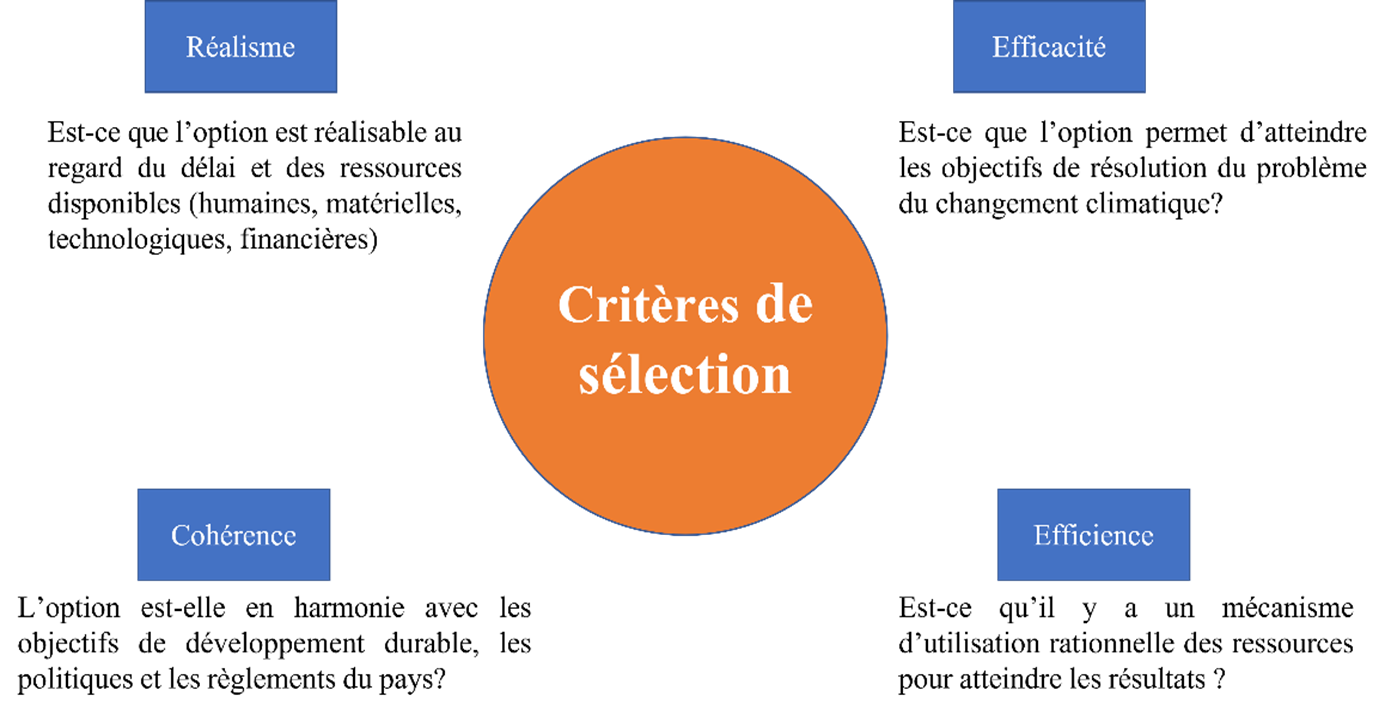
\includegraphics{Figures and Photos/Figure 22.png}
\caption{\textbf{Figure 22: Criteria for Selecting Adaptation Options}}
\end{figure}

\emph{Source: Consultant for the revision of the NAP}

\subsection{Water resources sector}\label{water-resources-sector}

The overall objective of the NAP in the water resources sector is to: \textbf{``Strengthen the resilience of water resources to the adverse effects of climate change''}.

Specifically, these are:

\begin{itemize}
\item
  strengthen the resilience of water resource mobilization structures;
\item
  ensure integrated water resources management;
\item
  improve knowledge of water resources.
\end{itemize}

The adaptation measures being considered and their impacts are described below.

\begin{tabular}{>{\raggedright\arraybackslash}p{30em}|>{\raggedright\arraybackslash}p{30em}|>{\raggedright\arraybackslash}p{30em}|>{\raggedright\arraybackslash}p{30em}|>{\raggedright\arraybackslash}p{30em}|>{\raggedright\arraybackslash}p{30em}}
\hline
\multicolumn{6}{c}{Table 6: Synthesis of adaptation measures and their impacts in the water resources sector} \\
\cline{1-6}
Climate Risks &   & Accomodations & Description & Expected Impacts & Timeline\\
\hline
Flood & Physics & Protecting water resource mobilization structures & Ensure the upkeep and maintenance of water resource mobilization facilities;                 Protecting the banks of rivers and bodies of water;                      Delineate easement strips & Improves water availability & Short-term\\
\hline
 &  &  &  &  \vphantom{5} & \\
\hline
 & Strategic & Protecting water resource mobilization structures & Monitor compliance with easement bands & Improves the availability of water resources & Short-term\\
\hline
 &  & Improving hydrological forecasting & Strengthening the national water information system & Improving the protection of water resource mobilization structures & \\
\hline
 & Institutional & Strengthening water quality monitoring & Strengthening the capacity of water agencies;              Strengthen water quality monitoring systems to help reduce the impact of flooding by ensuring that water resources are not contaminated & Improves water quality & Short-term\\
\hline
 &  &  &  &  \vphantom{4} & \\
\hline
Drought & Physics & Mobilizing water resources & Construct dams, basins, reservoirs and underground aquifers to provide a source of water during periods of drought & Improves the availability of water resources & Long-term\\
\hline
 &  & Restoring wetlands & Carry out cleaning of the plans; Protecting the banks of rivers and bodies of water;                     Delineate easement strips & Improves the availability of water resources & Short-term\\
\hline
 &  &  &  &  \vphantom{3} & \\
\hline
 & Strategic & Ensuring integrated water resources management & Reduce non-essential water use, and improve water use efficiency and promote water conservation; Reuse and recycle water; Strengthening the capacities of Local Water Committees & Improves the availability of water resources & Short-term\\
\hline
 &  &  &  &  \vphantom{2} & \\
\hline
 &  &  &  &  \vphantom{1} & \\
\hline
 &  & Improving knowledge of water resources & Develop information documents on water resources;                      Acquire equipment that contributes to the knowledge of water resources;                                Carry out studies on the knowledge of water resources;                  Carry out water level gauging campaigns & Improves water resource management & Short-term\\
\hline
 &  &  &  &  & \\
\hline
 & Institutional & Improving hydrological forecasting & Strengthening the national water information system & Improving the rational management of water resources & Short-term\\
\hline
High temperatures & Physics & Protecting water resource mobilization structures & Carry out reforestation;          Protecting the banks of streams and bodies of water & Reduce the effect of evapotranspiration and increase water availability & Short-term\\
\hline
 & Strategic & Ensuring rational management of water resources & Prioritizing the use of water resources in times of high heat & Improves the availability of water resources. & Short-term\\
\hline
 & Institutional & Communication, Education and Community Outreach & Build community capacity on the impacts of extreme heat on water resources and promote water-saving measures & Reduce pressure on water resources and improve resilience to extreme heat conditions. & Short-term\\
\hline
\end{tabular}

\emph{Source: Consultant for the revision of the NAP}

\subsection{Agriculture sector}\label{agriculture-sector}

The overall objective of the NAP in the agriculture sector is to \textbf{``strengthen the resilience of farms to the adverse effects of climate change''}.

Specifically, these are:

\begin{itemize}
\item
  restore soil fertility to limit its continued degradation;
\item
  improve agricultural productivity;
\item
  strengthen the resilience capacities of populations affected by disasters (floods, drought, massive predator attacks, etc.);
\item
  develop early warning systems for efficient management of climate variability and change.
\end{itemize}

The adaptation measures being considered and their impacts are described below.

\begin{tabular}{>{\raggedright\arraybackslash}p{30em}|>{\raggedright\arraybackslash}p{30em}|>{\raggedright\arraybackslash}p{30em}|>{\raggedright\arraybackslash}p{30em}|>{\raggedright\arraybackslash}p{30em}|>{\raggedright\arraybackslash}p{30em}}
\hline
\multicolumn{6}{c}{Table 7: Synthesis of adaptation measures and their impacts in the agriculture sector} \\
\cline{1-6}
Climate Risks &   & Accomodations & Description & Expected Impacts & Timeline\\
\hline
Flood & Physics & Drainage system & Establish a proper drainage system to keep water away from fields and crops;                 Promote the use of stormwater collection ponds (RWS) to control the flow of water on farms & Helps manage excess water and redirect it away from field crops & Short-term\\
\hline
 & Strategic & Flood-tolerant crop varieties & Use seed varieties that are more resistant to flooding & Reduces crop loss and increases yield & Short-term\\
\hline
 &  &  & Developing varieties that adapt to flooding &  & Medium-term\\
\hline
 &  & Soilless cultivation & Promote the practice of soilless agriculture to control the flow of water over crops & Reduces crop loss and increases yield & Long-term\\
\hline
 &  & Crop rotation & Rotate the type of crops grown in the same field each year to reduce soil saturation & Improves water drainage by reducing soil compaction and increasing soil porosity & Short-term\\
\hline
 & Institutional & Early warning systems & Establish early warning systems to warn farmers of the occurrence of floods, allowing them to prepare for and protect their crops & Reduces crop loss and also contributes to the safety of farmers and their families & Short-term\\
\hline
Drought & Physics & Water Conservation Techniques & Improve on-farm water management through rainwater harvesting, soil moisture monitoring and water-efficient irrigation systems to optimize water use & Makes water available for crops in times of drought and prevents crop failures & Short-term\\
\hline
 &  & Short-cycle varieties & Use improved short-cycle varieties to reduce the need for water for product maturation & Reduces production losses and ensures yields & \\
\hline
 & Strategic & Irrigation systems & Promote surface irrigation, sprinkler irrigation and drip irrigation systems & Ensures plants' water needs while reducing waste & Short-term\\
\hline
 &  & Drought-tolerant crops & Develop improved seeds adapted to drought & Improves crop yield and resilience, reduces water input to crops & Long-term\\
\hline
 &  & Smart Farming & Promote conservation agriculture, agroforestry and agroecology & Improves crop yield, soil fertility, water efficiency and also farmers' income & Medium-term\\
\hline
 & Institutional & Agricultural insurance & Promote index-based insurance for agricultural products as well as the subscription to African risk capacity agricultural insurance & Compensate for losses and reduce the financial impact of drought on producers and the country;                                     Improves adaptation to drought-related climate change & Medium-term\\
\hline
High temperatures & Physics & Infrastructure Improvements & Build infrastructure, such as greenhouses and elevated tunnels, to help reduce the impact of extreme heat on crops and protect them from damage & Protect crops from extreme temperatures and heat waves & Medium-term\\
\hline
 & Strategic & Soil Management & Promote conservation agriculture and the use of organic matter to help regulate soil temperature and moisture levels. This makes crops more resistant to heat stress & Improves soil properties and reduces the risk of crop drying out during long periods of heat & Short-term\\
\hline
 &  & Heat Stress Resistant Crops & Develop and promote improved seeds that are more resistant to heat & Maintain crop productivity even in extreme temperatures, resulting in higher yields and increased profits & Short-term\\
\hline
 & Institutional & Communication, Awareness, Education & Build farmers' capacity to help them make informed decisions to improve the resilience of their crops to extreme heat & Develop more resilient agricultural practices and use new technologies to adapt crops to high temperatures & Medium-term\\
\hline
\end{tabular}

\emph{Source: Consultant for the revision of the NAP}

\subsection{Livestock sector and fisheries resources}\label{livestock-sector-and-fisheries-resources}

The NAP for the livestock and fisheries sector has set an overall objective of \textbf{``reducing the vulnerability of agro-pastoralists and pastoral and fisheries resources to the adverse effects of climate change''}.

Specifically, these are:

\begin{itemize}
\item
  improve animal and fisheries health;
\item
  increase the productivity of animal and fisheries resources;
\item
  improve the availability and accessibility of animal feed;
\end{itemize}

In the area of livestock and fisheries resources, adaptation measures and expected impacts are described below.

\begin{tabular}{>{\raggedright\arraybackslash}p{30em}|>{\raggedright\arraybackslash}p{30em}|>{\raggedright\arraybackslash}p{30em}|>{\raggedright\arraybackslash}p{30em}|>{\raggedright\arraybackslash}p{30em}|>{\raggedright\arraybackslash}p{30em}}
\hline
\multicolumn{6}{c}{Table 8 : Synthesis of adaptation measures and their impacts in the livestock and fisheries resources sector} \\
\cline{1-6}
Climate Risks &   & Accomodations & Description & Expected Impacts & Timeline\\
\hline
Flood & Physics & Building water collection points;                   Protecting water points from silting up and eutrophication;                                         Construct fishways at weirs to protect fish during flooding & Install a drainage system and create water points to collect surplus water that can be used for livestock;                                                   Protect the banks to prevent flooding from silting up and eutrophicating watercourses and endangering fish stocks;                                 Protecting fish from sudden and dangerous falls during floods & Relieve congestion in pastoral infrastructure and create water reservoirs to alleviate water dependence in times of drought and high heat for the population and livestock;                      Reduces silting and eutrophication of watercourses;                                              Reduces fish mortality at weirs & Short-term\\
\hline
 & Strategic & Developing early warning systems & Inform agro-pastoralists in real time about the occurrence of a flood & Reduces the impact of flooding through prevention & Short-term\\
\hline
 & Institutional & Improving the harmonious development of fish & Setting up measures to preserve fisheries resources & Reduces resource loss & Short-term\\
\hline
Drought & Physics & Improving the availability of fodder; Improving the availability of water in pastoral areas and increasing the retention capacity of water reservoirs & Cultivate, mow and conserve natural fodder to compensate for the lack of livestock feed;            Carry out pastoral boreholes and boulis;                  Carry out actions to restore water bodies & Reduces animal mortality during droughts & Short-term\\
\hline
 & Strategic & Transforming pastoral areas into livestock production intensification zones (ZIPA);  Develop a plan for the restoration of degraded pastures & Build pastoral infrastructure and carry out actions to secure land, food and health; Recovering degraded land and replenishing vegetation cover through ESC/DRS techniques and the sedentarization of herds & Promotes the harmonious development of livestock farming;                                   Increase forage biomass and soil water infiltration and GHG sequestration & Short-term\\
\hline
 & Institutional & Improving animal health & Systematically vaccinate and deworm animals & Reduces vulnerability to the effects of drought & Short-term\\
\hline
High temperatures & Physics & Use Heat Stress Relievers & Providing anti-stress heat medication for animals & Increases animal resistance & Short-term\\
\hline
 & Strategic & Practise sedentarisation & Keeping livestock in a fixed location to withstand heat waves and associated diseases & Reduces livestock mortality & \\
\hline
 & Institutional & Develop communication, outreach and community education & Building community capacity on the impacts of extreme heat on animal resources and promoting adaptation measures & Help improve resilience to extreme heat conditions. & Medium-term\\
\hline
\end{tabular}

\emph{Source: Consultant for the revision of the NAP}

\subsection{Environment/Natural Resources Sector}\label{environmentnatural-resources-sector}

The overall objective of the NAP for the environment and natural resources sector is to \textbf{``Strengthen the adaptive capacities of forest ecosystems, including wildlife, to the adverse effects of climate change''}.

Specifically, these are:

\begin{itemize}
\item
  strengthen the adaptive capacity of wildlife resources;
\item
  improve the conservation and protection of forest and wildlife resources;
\item
  promote research and development actions and resilient practices to increase forest resources.
\end{itemize}

For the Environment/Natural Resources sector, adaptation measures and their impacts are described below.

\begin{tabular}{>{\raggedright\arraybackslash}p{30em}|>{\raggedright\arraybackslash}p{30em}|>{\raggedright\arraybackslash}p{30em}|>{\raggedright\arraybackslash}p{30em}|>{\raggedright\arraybackslash}p{30em}|>{\raggedright\arraybackslash}p{30em}}
\hline
\multicolumn{6}{c}{Table 9: Synthesis of adaptation measures and their impacts in the Environment/Natural Resources sector} \\
\cline{1-6}
Climate Risks &   & Accomodations & Description & Expected Impacts & Timeline\\
\hline
Flood & Physics & Improving drainage systems & Rehabilitating water infrastructure;                 Construct stormwater and runoff drainage channels & Reduces the destruction of biotopes and the loss of biological diversity & Medium-term\\
\hline
 &  & Improving the conservation and restoration of forest resources & Producing and planting species adapted to flood-prone areas; Restoring vegetation cover; Strengthening systems to protect forest resources from flooding & Reduces the destruction of biotopes and the loss of biological diversityImproves vegetation coverImproves the income of vulnerable populations & Short-term\\
\hline
 & Strategic & Improving weather and hydrological forecasting; Promoting seed varieties adapted to flood-prone areas & Strengthening the climate change early warning system; Developing and disseminating seeds adapted to flood-prone areas & Reduces the potential impacts of flooding on resources; Increases the survival rate of planted plants & Short-term\\
\hline
 & Institutional & Improving the availability of climate, hydrological and meteorological information & Strengthening the ANAM and DGRE observation network; Improving the framework for consultation between the various actors & Improves the reliability and availability of climate, hydrological and meteorological  information to facilitate decision-making. & Short-term\\
\hline
Drought & Physics & Promoting sustainable land management; Strengthening forest management & Promote the use of ESC/DRS techniques and other good SLM practices; Promote the use of techniques for the conservation and protection of forest resources; Carry out reforestation & Improves soil fertility in forest ecosystems; Improves forest resilience and biodiversity conservation & Short-term\\
\hline
 &  & Improving Water Conservation and Availability in Wildlife Protection Areas (FPAs) & Construct and rehabilitate water mobilization structures & Reduces water stress in PFAs and contributes to the reduction of wildlife mortality & \vphantom{1} Medium-term\\
\hline
 & Strategic & Promoting drought-tolerant forest seed varieties & Developing and Expanding Drought-Adapted Forest Seeds & Increases the survival rate of planted plants & Medium-term\\
\hline
 & Institutional & Developing early warning systems & Strengthen the partnership with the actors of the warning system and strengthen the early warning system on bushfires & Prevent bushfires and reduce biodiversity loss & Short-term\\
\hline
High temperatures & Physics & Improving forest potential & Carry out reforestation; Promote the use of techniques for the conservation and protection of forest resources & Contributes to the preservation of ecosystems during hot weather & Short-term\\
\hline
 &  & Improving Water Conservation and Availability in Wildlife Protection Areas (FPAs) & Construct and rehabilitate water mobilization structures & Reduces water stress in PFAs and contributes to the reduction of wildlife mortality & Medium-term\\
\hline
 & Strategic & Promoting forest seed varieties adapted to high temperatures & Developing and disseminating forest seeds adapted to high temperatures & Increases the survival rate of planted plants and reduces water stress & Medium-term\\
\hline
 & Institutional & Develop communication, outreach and community education & Building community capacity on the impacts of extreme heat on forest resources and promoting adaptation measures & Help improve resilience to extreme heat conditions & Medium-term\\
\hline
\end{tabular}

\emph{Source: Consultant for the revision of the NAP}

\subsection{Health sector}\label{health-sector}

\subsubsection{Adaptation Priority Areas}\label{adaptation-priority-areas}

The expected adverse effects of climate change call for targeted actions to reduce them. Thus, the overall objective of \textbf{``Strengthening the capacity of the health sector to adapt to climate change, for better protection of the population''} has been set for the sector in the face of the effects of climate change. Depending on the foreseeable climate shocks and their impacts, the proposed adaptation actions are as follows:

\begin{itemize}
\item
  improve the planning system within the Ministry of Health (MOH) in a gender- and equity-sensitive manner;
\item
  establish/strengthen appropriate frameworks for consultation, health development planning and communication between the MOH and other actors at all levels;
\item
  develop a national strategy for continuing education with consolidated plans for continuing education at all levels of the health system;
\item
  implement communication plans for health;
\item
  strengthen the surveillance system at all levels;
\item
  build new health infrastructure that meets standards by level;
\item
  strengthen the operational capacity of the MS in research;
\item
  advocate for an increase in the share of the state budget allocated to health.
\end{itemize}

In the health sector, the potential impacts and adaptation measures to be taken over time are described below.

\begin{tabular}{>{\raggedright\arraybackslash}p{30em}|>{\raggedright\arraybackslash}p{30em}|>{\raggedright\arraybackslash}p{30em}|>{\raggedright\arraybackslash}p{30em}|>{\raggedright\arraybackslash}p{30em}|>{\raggedright\arraybackslash}p{30em}}
\hline
\multicolumn{6}{c}{Table 10: Synthesis of adaptation measures and their impacts in the health sector} \\
\cline{1-6}
Climate Risks &   & Accomodations & Description & Expected Impacts & Timeline\\
\hline
Flood & Physics & Building Flood-Resistant Health Facilities & Use of flood-resistant building materials and integration of efficient drainage systems & Reduced damage to medical equipment and supplies & Long-term\\
\hline
 & Strategic & Improving access to health care & Have mobile care units, storage of medical supplies in flood-prone areas & Access to care and also to essential medicines & Short-term\\
\hline
 & Institutional & Integrating disaster management & Integrate health into disaster management plans to ensure a coordinated response to floods & Integration allows for a coordinated and well-planned response by disaster management agencies and the health sector & Short-term\\
\hline
Drought & Physics & Making Power Available & Lack of food due to drought can lead to acute mortality, especially among children & This system will improve the health of the population and kick-start the country's development & Short-term\\
\hline
 & Strategic & Making emergency emergency food stocks available & These stocks will make up for food shortages in a timely manner & The health of the population will be improved & Short-term\\
\hline
 & Institutional & Institutionalizing free or subsidized provision to the poorest in times of severe drought & These provisions will make it possible to be efficient in real time & The health of the population will be improved & Short-term\\
\hline
High heat & Physics & Improving health care infrastructure & Modernize health care infrastructure, including air conditioning and ventilation systems & Allows vaccines and medicines to be stored at a recommended temperature in case of high heat & Long-term\\
\hline
 & Strategic & Promoting Healthy Behaviours & Encourage people to adopt healthy behaviours, such as staying hydrated, seeking shade, and avoiding outdoor activities during the hottest hours of the day & Reducing the risk of heat-related illnesses & Short-term\\
\hline
 &  & Improving access to health care & Increase the availability of medical services, particularly during the warmer months, to manage heat-related health issues & Greater patient satisfaction, as they can receive prompt and effective treatment for heat-related illnesses & Short-term\\
\hline
\end{tabular}

\emph{Source: Consultant for the revision of the NAP}

\subsection{Energy sector}\label{energy-sector}

The overall objective of the NAP for the energy sector is to \textbf{``improve the adaptive capacity of the energy sector to the adverse effects of climate change''}.

Specifically, these are:

\begin{itemize}
\item
  develop resilient energy transport and storage infrastructure;
\item
  promote energy efficiency;
\item
  promoting renewable energy and hydropower;
\item
  the decline in thermal electricity production;
\item
  the reduction of wood energy;
\item
  the development of energy transport and storage infrastructure;
\item
  the development of hydropower generation;
\item
  control of energy consumption.
\end{itemize}

Adaptation measures and their impacts in the energy sector are described below.

\begin{tabular}{>{\raggedright\arraybackslash}p{30em}|>{\raggedright\arraybackslash}p{30em}|>{\raggedright\arraybackslash}p{30em}|>{\raggedright\arraybackslash}p{30em}|>{\raggedright\arraybackslash}p{30em}|>{\raggedright\arraybackslash}p{30em}}
\hline
\multicolumn{6}{c}{Table 11: Synthesis of adaptation measures and their impacts in the energy sector} \\
\cline{1-6}
Climate Risks &   & Accomodations & Description & Expected Impacts & Timeline\\
\hline
Flood & Physics & Strengthening the protection of energy infrastructure & Install facility protection systems; Implement a stormwater and runoff drainage system to protect energy facilities & Reduce the risk of equipment destruction & Long-term\\
\hline
 & Strategic & Identify suitable sites for the implementation of infrastructures; Promoting resilient infrastructure models & Conduct technical studies necessary for the installation of infrastructure;                     Design and/or acquire flood-resistant energy equipment & Lower repair costs and increased reliability of the energy sector in the event of equipment flooding;             Reduces technical breakdowns and supply disruptions & Short-term; Long-term\\
\hline
 & Institutional & Early Warning System & Strengthen the partnership with the actors of the alert system and strengthen the early warning system & Reduces the risk of equipment damage and network disruptions & Short-term\\
\hline
Drought & Physics & Developing technologies to compensate for the use of wood energy & Promoting Improved Cookstoves for the Benefit of Households;                          Promoting the use of biogas & Reduces overexploitation of forest resources as an energy source & Short-term\\
\hline
 & Strategic & Implement an electrical energy saving strategy & Promote the acquisition of energy-efficient lighting fixtures and systems;                Development of awareness and education programs on gestures and habits leading to electrical energy savings;                         Promoting the use of solar energy equipment & Reduces the consumption of fossil fuels & Long-term\\
\hline
 & Institutional & Promoting renewable energy; Early Warning System & Encouraging the use of renewable energy such as solar, which is less vulnerable to drought, can help mitigate the effects of drought on energy production;            Strengthen the partnership with the actors of the warning system and strengthen the early warning system to respond more effectively to droughts & Renewable energy sources such as solar energy do not need water to generate electricity;                        Reduces disruption to the network & Long-term;    Short-term\\
\hline
High temperatures & Physics & Use suitable electrical appliances & Acquire equipment and devices that are resistant to high temperatures & Strengthens energy supply by maintaining energy production and availability & Short-term\\
\hline
 & Strategic & Strengthening the energy mix & Diversify energy sources to improve electricity supply;                               Implement incentives for the acquisition and use of solar equipment & Reduces the use of thermal energy & Short-term\\
\hline
 & Institutional & Early Warning System & Strengthen the partnership with the actors of the alert system and strengthen the early warning system to react more effectively to high temperatures & Respond effectively to high temperatures, thus reducing the risk of technical breakdowns & Short-term\\
\hline
\end{tabular}

\emph{Source: Consultant for the revision of the NAP}

\subsection{Infrastructure and housing sector}\label{infrastructure-and-housing-sector}

The overall objective of the NAP for the infrastructure and housing sector is \textbf{``Strengthening the resilience of infrastructure and habitats to the effects of climate change''}.

Specifically, it involves:

\begin{itemize}
\item
  reduce the vulnerability of community social infrastructure and facilities;
\item
  promote housing that is resilient to the effects of CCs;
\item
  strengthen planning and construction standards.
\end{itemize}

In the infrastructure and housing sector, adaptation measures and their impacts are described below.

\begin{tabular}{>{\raggedright\arraybackslash}p{30em}|>{\raggedright\arraybackslash}p{30em}|>{\raggedright\arraybackslash}p{30em}|>{\raggedright\arraybackslash}p{30em}|>{\raggedright\arraybackslash}p{30em}|>{\raggedright\arraybackslash}p{30em}}
\hline
\multicolumn{6}{c}{Table 12: Synthesis of adaptation measures and their impacts in the infrastructure and housing sector} \\
\cline{1-6}
Climate Risks &   & Accomodations & Description & Expected Impacts & Timeline\\
\hline
Flood & Physics & Build urban infrastructure and equipment with materials that adapt to flooding & Build urban infrastructure and equipment that adapts to flooding; Construct and rehabilitate stormwater drainage and runoff structures in urban areas & Increasing the resilience of infrastructure and equipment to flooding & Long-term\\
\hline
 & Strategic & Promote the use of materials that adapt to flooding in the construction of urban infrastructure and equipment;  Promote the use of innovative models for the construction of habitats & Acquire or encourage the acquisition of materials that adapt to flooding through the implementation of incentives and awareness campaigns; Promote the use of plan-typical, cut laterite bricks & Increasing the resilience of infrastructure, equipment and populations to flooding;   Improves quality of life & Medium-term\\
\hline
 & Institutional & Implement a programme for the resorption and restructuring of spontaneous habitats;                                   Increase the monitoring and control of constructions;                                         Communication, Education and Outreach & Construct drainage works and easement areas in neighbourhoods to deal with flooding ;                     Ensure compliance with building standards;      Ensure compliance with the specifications for the construction of infrastructures;                            Ensure compliance with building regulations concerning (i) the construction of water infrastructure, roads, human settlements, (ii) the occupation of space in urban and rural areas and in particular flood zones, (iii) industrial activities;                             Strengthen people's knowledge of the impacts of climate change on the infrastructure and housing sector & Improves quality of life;                             Reduces the degradation and destruction of infrastructure and equipment in the face of flooding;                                              Increasing people's resilience to flooding & Long-term;                    Short-term;                  Medium-term\\
\hline
 &  &  &  &  \vphantom{3} & \\
\hline
 &  &  &  &  \vphantom{2} & \\
\hline
Drought & Physics & Constructing urban infrastructure and equipment with materials that adapt to drought & Building urban infrastructure and facilities that adapt to drought & Increasing the resilience of infrastructure and equipment to drought & Long-term\\
\hline
 & Strategic & Promoting the Green Cities Agenda;          Promote the use of innovative models for the construction of habitats & Promote the systematic planting of drought-adapted plant species;                                            Promote the use of plan-types, cut laterite bricks, tiles & Increasing people's resilience to drought & Short-term\\
\hline
 &  &  &  &  \vphantom{1} & \\
\hline
 & Institutional & Communication, Education and Outreach & Strengthen people's knowledge of the impacts of climate change on the infrastructure and housing sector & Increasing people's resilience to drought & Short-term\\
\hline
High temperatures & Physics & Build urban infrastructure and equipment in materials that adapt to high temperatures; Carry out alignment plantings & Building urban infrastructure and equipment that adapts to high temperatures;                           Plant shade species that promote the fixation of the pavement & Increasing the resilience of infrastructure and equipment in the face of high temperatures;                                    Increasing the resilience of infrastructure and equipment in the face of high temperatures & Long-term;                 Short-term\\
\hline
 & Strategic & Promote the use of eco-friendly materials for the construction of urban infrastructure and equipment;                                         Promoting the Green Cities Agenda;                              Promote the use of ecological models for the realization of habitats & Encourage the use of eco-friendly materials through incentives;                                          Promote the systematic planting of plant species adapted to high temperatures;                                Promote the use of standard plans, cut laterite bricks, tiles to cope with high temperatures & Increasing the resilience of infrastructure, equipment and populations in the face of extreme heat & Medium-term; Short-term\\
\hline
 &  &  &  &  & \\
\hline
 & Institutional & Developing a fire alarm system in collective social infrastructures;                             Communication, Education and Outreach & Strengthen the partnership with the actors of the alert system and create the fire alarm system to react more effectively to fires in social and collective infrastructures occurring during high temperatures;                                                  Strengthen people's knowledge of the impacts of climate change on the infrastructure and housing sector & Reduces the risk of infrastructure destruction;                                          Increasing the resilience of populations in the face of extreme heat & Long-term; Medium-term\\
\hline
\end{tabular}

\emph{Source: Consultant for the revision of the NAP}

\subsection{Gender theme}\label{gender-theme}

\subsubsection{Adaptation Priority Areas}\label{adaptation-priority-areas-1}

The overall objective of \textbf{``Contribute to improving the resilience of members of women's associations through the implementation of income-generating activities''} is the one set in the sector in the face of the effects of climate change. To cancel out the vulnerability factors, the following adaptation actions are proposed:

Specifically, these are:

\begin{itemize}
\item
  capacity building of women's associations on good practices for adaptation to climate change;
\item
  improving women's access to safe drinking water during water shortages;
\item
  raising women's awareness of the nutritional values of NTFPs for better preservation and enhancement of the species that provide them;
\item
  strengthening women's technical capacities on good harvesting and processing practices and on provisions to ensure natural and assisted regeneration;
\item
  the promotion of income-generating activities for women. In the area of gender, the potential impacts and adaptation measures to be taken over time are described below.
\end{itemize}

\begin{tabular}{>{\raggedright\arraybackslash}p{30em}|>{\raggedright\arraybackslash}p{30em}|>{\raggedright\arraybackslash}p{30em}|>{\raggedright\arraybackslash}p{30em}|>{\raggedright\arraybackslash}p{30em}|>{\raggedright\arraybackslash}p{30em}}
\hline
\multicolumn{6}{c}{Table 13 : Synthesis of adaptation measures and their impacts in the Gender theme} \\
\cline{1-6}
Climate Risks &   & Accomodations & Description & Expected Impacts & Timeline\\
\hline
Flood & Physics & Building flood-resilient socio-economic infrastructure for women's organizations & The construction of flood-resilient markets, tracks and shops will allow women's associations to continue to carry out their activities in the event of flooding & The impacts are positive in the sense that they will allow women's associations to continue to carry out their activities & Long-term\\
\hline
 & Strategic & Develop a plan to strengthen the resilience of women's associations & Members of women's associations will receive adequate training on what to do in the event of a flood & The knowledge gained will enable them to protect against the adverse effects of flooding & Short-term\\
\hline
 & Institutional & Include a budget line for the financing of resilience measures for members of women's associations in the event of flooding & Flood resilience initiatives will be supported for their implementation & There will be an effective implementation of Climate Change adaptation initiatives by members of women's associations & Short-term\\
\hline
Drought & Physics & Construct hydraulic infrastructure (dams, boulis, boreholes, etc.) & Women's associations generally engage in market gardening activities (off-season crops) & This practice will allow them to produce in times of water scarcity and boost local economies & Long-term\\
\hline
 & Strategic & Promote awareness-raising plans on good practices for adapting to climate change & The popularization of climate change adaptation tools and measures will increase the level of resilience of women's associations & Women's associations will find solutions to continue carrying out activities & Short-term\\
\hline
 & Institutional & Have the gender theme taken into account in the budget forecasts of the State or municipalities & The availability of financial resources will allow for timely action & Income from women's associations' income-generating activities will improve & Short-term\\
\hline
High temperatures & Physics & Carry out reforestation for shade & The availability of shade for members of women's associations will allow them to continue activities in good health & The health of members of women's associations will be improved & Long-term\\
\hline
 & Strategic & Draw up an information leaflet on the harmful effects of high temperatures on members of women's associations & Knowing this information will raise awareness & The health of members of women's associations and IGAs will be improved & Short-term\\
\hline
 & Institutional & Establish a follow-up of the activities of the members of women's associations & The monitoring of the working conditions of members of women's associations in the context of climate change will be carried out & Members of women's associations will be less vulnerable to illnesses due to heat peaks & Short-term\\
\hline
\end{tabular}

\emph{Source: Consultant for the revision of the NAP}

\subsection{Thematic Civil Society Organisations (CSOs)}\label{thematic-civil-society-organisations-csos}

\subsubsection{Adaptation Priority Areas}\label{adaptation-priority-areas-2}

The overall objective of \textbf{``Improving the resilience capacities of women's organizations in an inclusive manner for better governance in the implementation of NAP/CC in Burkina Faso''} is set in the theme facing the effects of climate change.

Specifically, these are:

\begin{itemize}
\item
  strengthen the technical capacities of women's organizations on good adaptation practices;
\item
  consolidate/strengthen the organizational capacities of women's organizations;
\item
  increase the resource mobilization capacity of women's organizations;
\item
  take women's organizations into account in consultation frameworks related to adaptation to climate change;
\item
  promote income-generating activities for women.
\end{itemize}

In the field of CSOs, the potential impacts and adaptation measures to be taken over time are described below.

\begin{tabular}{>{\raggedright\arraybackslash}p{30em}|>{\raggedright\arraybackslash}p{30em}|>{\raggedright\arraybackslash}p{30em}|>{\raggedright\arraybackslash}p{30em}|>{\raggedright\arraybackslash}p{30em}|>{\raggedright\arraybackslash}p{30em}}
\hline
\multicolumn{6}{c}{Table 14 : Synthesis of adaptation measures and their impacts in the theme of civil society organizations} \\
\cline{1-6}
Climate Risks &   & Accomodations & Description & Expected Impacts & Timeline\\
\hline
Flood & Physics & Supporting Women's Organizations (FOs) to build flood-resistant infrastructure & The construction of flood-resilient premises, runways, and shops will allow women's associations to continue to carry out their activities in the event of flooding & Women's organizations can continue to offer their services and continue to carry out their activities even in the event of flooding & Long-term\\
\hline
 & Strategic & Develop an integrated plan for mobilizing and strengthening the capacities of women's organizations & The aim is to have a tool that will facilitate the involvement and capacity building of women's organizations;                                           Members of women's associations will receive adequate training on what to do in the event of a flood & The knowledge acquired will enable them to protect themselves from the harmful effects of floods;                  The contribution of women's organizations to climate change efforts will be increased & Short-term\\
\hline
 & Institutional & Supporting the structuring of women's organizations;                              Setting up a consultation framework for women's associations & The aim is to strengthen the organisation and governance of women's organisations to respond to the challenges of climate change & There will be a critical mass of women's organizations contributing to the fight against the adverse effects of climate change & Short-term\\
\hline
 &  &  &  &  \vphantom{1} & \\
\hline
Drought & Physics & Support or facilitate the construction of hydraulic infrastructure (boulis, boreholes, etc.) for the benefit of the FOs & The construction of the structures will allow women's associations to continue to carry out their activities even in the event of droughts & The construction of hydraulic structures will increase the mobilization of water resources;                                Women's associations will be able to practice market gardening activities (off-season crops) & Long-term\\
\hline
 & Strategic & Develop an integrated plan for mobilizing and strengthening the capacities of women's organizations & The aim is to have a tool that will facilitate the involvement and capacity building of women's organizations & The knowledge acquired will enable the OFs to cope with and anticipate droughts & Short-term\\
\hline
 & Institutional & Strengthen the organizational capacities of FOs to deal with droughts;                                  Establish mechanisms or partnerships that facilitate access to alerts by the work orders & It is a question of organising the OFs or supporting them to structure themselves in order to be able to respond to droughts & We will have more organized and structured FOs that are able to cope with droughts & Short-term\\
\hline
 &  &  &  &  & \\
\hline
High temperatures & Physics & Carry out reforestation for shade & The availability of shade for members of women's associations will allow them to continue activities in good health & The effects of heat on the lives of women's associations will be reduced & Long-term\\
\hline
 & Strategic & Establish facilities or mechanisms to finance reforestation activities in FOs & The aim is to facilitate the access of FOs to financial resources to implement their reforestation activities & FOs will be quick to implement reforestation initiatives & Short-term\\
\hline
 & Institutional & Establish mechanisms or partnerships that facilitate FOs' access to heatwave alerts & The aim is to facilitate access to alerts and information on high temperatures for foreign nationals & Members of women's associations will anticipate measures to cope with the high heat and will be less vulnerable to illnesses due to heat peaks & Short-term\\
\hline
\end{tabular}

\emph{Source: Consultant for the revision of the NAP}

\section{Costs and benefits of adaptation options}\label{costs-and-benefits-of-adaptation-options}

In the process of developing Burkina Faso's first NAP, the T21 multi-sectoral modelling tool was used. Integrated, long-term scenarios have been generated by the T21-Burkina Faso model to study policy proposals that can contribute to climate change resilience. In this model, the adaptation policies tested concerned the sectors of agriculture, livestock, energy, health, environment, human habitats/infrastructure/natural disasters. Table 15 provides an overview of adaptation policies.

\begin{tabular}{>{\raggedright\arraybackslash}p{30em}|>{\raggedright\arraybackslash}p{30em}}
\hline
\multicolumn{2}{c}{Table 15 : Adaptation Policies in the T21 Burkina Faso Model} \\
\cline{1-2}
Sector & Policies\\
\hline
Agriculture & Technology \& Awareness\\
\hline
Breeding & Transition to More Intensive Systems \& Awareness\\
\hline
Health & Treatment \& Prevention\\
\hline
Energy & Photovoltaic; Air Conditioning Efficiency Solar Cooker Hydroelectricity; Improved cookstoves; Other\\
\hline
Environment & Reforestation; Construction of dams\\
\hline
Human Habitat / Infrastructure / Natural Disasters & Reconstruction of flood damage; Prevention - construction of gutters; Prevention - awareness\\
\hline
\end{tabular}

\emph{Source: Burkina Faso Programmatic NAPA Preparation Document}

Based on this analysis, short-, medium- and long-term (1 to 15 years) climate change adaptation options were proposed for each of the development sectors covered by the NAP. This analysis makes it possible to highlight the accumulated costs of investments in relation to GDP, for adaptation for the period (2014-2050) and the benefits derived from them.

For the intermediate scenario, optimization simulations showed that 0.7\% of GDP each year is needed to offset the negative impacts of climate change. In the worst-case scenario, it is even 1.5\% of GDP each year. It also shows the optimal distribution of these investments between the agriculture, livestock, energy, health, environment and human habitat/infrastructure/natural disasters sectors. The benefits of adaptation are the losses in GDP caused by climate change and avoided by adaptation.

This multi-sectoral vulnerability analysis work was carried out in 2012 with the aim of formulating a medium- and long-term national strategy for adaptation to climate change by 2025 and 2050 for Burkina Faso.

\begin{tabular}{>{\raggedright\arraybackslash}p{15em}|>{\raggedright\arraybackslash}p{15em}|>{\raggedright\arraybackslash}p{15em}}
\hline
\multicolumn{3}{c}{Table 16 : Unit costs for adaptation measures integrated into the T21-Burkina Faso model} \\
\cline{1-3}
Costs & Intermediate scenario & Worst-case scenario\\
\hline
Total Costs (2014-2050) & US\$4.5 billion & US\$9.6 billion\\
\hline
Agriculture: 35\% of investments & US\$1.58 billion & US\$3.36 billion\\
\hline
Livestock farming: 10\% of investments & US\$450 million & US\$960 million\\
\hline
Energy: 30\% of investments & US\$1.35 billion & US\$2.88 billion\\
\hline
Photovoltaics (50\%) & US\$675 million & US\$1.44 billion\\
\hline
Solar cooker (15\%) & US\$203 million & US\$432 million\\
\hline
Air conditioning efficiency (6\%) & US\$81 million & US\$173 million\\
\hline
Hydropower (5\%) & US\$68 million & US\$144 million\\
\hline
Improved Fireplace (1\%) & US\$14 million & US\$29 million\\
\hline
Other (23\%) & US\$311 million & US\$662 million\\
\hline
Healthcare: 5\% of investments & US\$225 million & US\$480 million\\
\hline
Environment: 10\% of investments & US\$450 million & US\$960 million\\
\hline
Reforestation (50\%) & US\$225 million & US\$480 million\\
\hline
Dam construction (50\%) & US\$225 million & US\$480 million\\
\hline
Human Habitat / Infrastructure / Natural Disasters: 10\% of investments & US\$450 million & US\$960 million\\
\hline
Reconstruction (60\%) & US\$270 million & US\$576 million\\
\hline
Prevention – construction of gutters (20\%) & US\$90 million & US\$192 million\\
\hline
Prevention – awareness (20\%) & US\$90 million & US\$192 million\\
\hline
Benefits &  & \\
\hline
Avoided GDP losses (2014 – 2050) & US\$28 billion & US\$55 billion\\
\hline
\end{tabular}

\emph{Source: Millennium Institute; www.millennium-institute.org}

So, in the intermediate scenario, the accumulated loss during the years (2014-2050) due to climate change is estimated at US\$28 billion, and in the worst-case scenario it is about US\$55 billion. This is a sum that is equal to seven times the GDP of the year 2008 (about US\$4 billion) for the intermediate scenario. For the worst-case scenario, this accumulated loss is nearly fourteen times the GDP of the year 2008.

In terms of adaptation, the cost of resilience measures should not be an obstacle to seeking funding for their implementation. The most important thing is to achieve the maximum benefit/cost ratio when implementing these measures. Although costly, these adaptation measures will reap many benefits for Burkina Faso's development, the main ones being summarized below:

\begin{itemize}
\item
  strengthening the resilience of agriculture and ecosystems;
\item
  securing pastoral activities and sustainable development of the pastoral economy;
\item
  greenhouse gas mitigation;
\item
  better health protection for the population;
\item
  women's improved access to natural resources and decision-making spaces;
\item
  etc.
\end{itemize}

More specifically, the expected economic and social benefits of the implementation of the NAP are as follows:

\begin{enumerate}
\def\labelenumi{\arabic{enumi}.}
\item
  \textbf{An increase in the production and incomes of rural populations:} the implementation of the NAP will contribute to reducing the vulnerability of natural, social and economic systems, which will lead to an increase in agro-sylvo-pastoral production and agricultural cash incomes of the population;
\item
  \textbf{A strong contribution to GDP:} reducing the vulnerability of natural, social and economic systems will strengthen the growth of the added value of each sector of the economy, and its contribution to the Gross Domestic Product (GDP);
\item
  \textbf{Creation of decent green jobs:} Production conditions will become conducive to investment, and the investments made will promote job creation in both the public and private sectors, especially for the youth. This means that it will then be possible to achieve an improvement in human well-being and social equity while significantly reducing environmental risks and resource scarcity.
\item
  \textbf{Knock-on effects for the rest of the economy:} the various development sectors concerned by the NAP represent the key sectors, and therefore the locomotives of Burkina Faso's development. The performance of these key sectors will have a clear knock-on effect on other sectors of the economy such as industry, trade and tourism.
\end{enumerate}

The conclusions of the Multisectoral Vulnerability Analysis for the Formulation of a Medium-and Long-Term National Climate Change Adaptation Strategy for Burkina Faso by 2025 and 2050 made in 2012 by the Millennium Institute during the training of Burkinabe executives on the T21 model showed that all development sectors in Burkina Faso are sensitive to climate change and all have vulnerability factors. The impact of climate change on these sectors is severe, and the cumulative losses in GDP until 2050 are in the billions if left unchecked. Moreover, the analysis reveals that the costs of adaptation are minimal compared to the benefits of adaptation; As a result, any delay in the implementation of adaptation strategies would increase costs.

Taking these analyses and conclusions into consideration within the framework of the NAP will enable Burkina Faso's economic emergence by greening the country's economy.

The various NAP sectoral plans have drawn up action plans for the implementation of priority actions. The total estimated costs of implementing these priority actions constitute the overall cost of implementing the NAP for the five (5) year period. The table in Annex 6 summarises the actions to be implemented by sector and the corresponding costs.

The overall budget for the implementation of the NAP for the five (5) year implementation period is estimated at: \textbf{Two hundred and eleven billion two hundred and thirty-three million eight hundred and seventy-nine thousand nine hundred and twenty-four (211,233,879,924) CFA francs}, of which \textbf{two hundred and eleven billion two hundred and six hundred and fifty-nine thousand eight hundred and ninety-eight (211,206,259,898) CFA francs} will be financed by the State, \textbf{twenty-four million nine hundred and sixty-one thousand five hundred (24,961,500 FCFA)} addressed to partners and the \textbf{remainder two thousand six hundred and fifty-eight thousand eighty (2,658,080 FCFA)} is to be sought.

\section{Mainstreaming climate change adaptation into development policies and strategies}\label{mainstreaming-climate-change-adaptation-into-development-policies-and-strategies}

The integration of climate change (CC), in the adaptation and mitigation components, into the development planning process at all levels represents a challenge for all countries and in particular for Burkina Faso and must be carried out in a proactive manner. Indeed, taking climate change into account in planning has been a recognized concern since the World Summit on Sustainable Development in Johannesburg in 2002, but little implemented in our context. This integration must go through two (2) processes:

\begin{enumerate}
\def\labelenumi{\arabic{enumi}.}
\item
  integrating climate change adaptation into planning;
\item
  integrating Climate Change Adaptation into budgeting.
\end{enumerate}

\subsection{Integrating Climate Change Adaptation into Planning}\label{integrating-climate-change-adaptation-into-planning}

The process of integrating climate change adaptation options into development policies, strategies, plans, programmes and projects requires an understanding of development policies, strategies, plans, programmes and projects, planning cycles and reflection on relevant adaptation options. The identification of entry points will point to adequate ``windows of opportunity'' for integration.

The entry points into the cycle of policies, strategies, plans, programmes and projects are as follows: (i) \textbf{planning:} transformation of issues and challenges into strategic directions and strategic axes; issues into global objectives and specific problems identified into specific objectives; root causes into strategic actions; and direct consequences or manifestations into results; (ii) \textbf{programming:} breakdown of actions relating to each programme/project, including climate-related activities, and projection of results targets over periods; and (iii) budgeting: the allocation of resources to planned activities.

\subsection{Integrating Climate Change Adaptation into Budgeting}\label{integrating-climate-change-adaptation-into-budgeting}

The inclusion of climate change in the budget is necessary for the implementation of climate change adaptation options contained in strategies, programmes and projects. As a result, it will be necessary to ensure that the budget allocation keys to be used are those that best enable the implementation of the strategic orientations resulting from the strategy papers and related to climate change.

The integration of climate change adaptation options into the budgeting process requires mastery of the steps of the budgeting process and the identification of entry points, which are ministries and other structures that can contribute to the success of the process. It will be necessary to draw up a list of the operations necessary for the fulfilment of each climate change adaptation option selected in the strategic development planning system, estimate the deadlines for implementation and evaluate the respective costs, with a view to their incorporation into the programming, budgeting and monitoring and evaluation instruments.

For a coherent integration of climate change adaptation into planning documents, a guide on the integration of climate change adaptation should be adopted to serve as a guiding document for the process and a national climate change committee should be set up to steer it.

\section{Operationalization of the National Adaptation Plan}\label{operationalization-of-the-national-adaptation-plan}

In order to operationalize the National Adaptation Plan, the following is a strategy comprising three (3) axes:

\begin{itemize}
\item
  Strategic axis 1: Strengthening the adaptive capacities of priority sectors;
\item
  Strategic axis 2: Research/Development on adaptation to climate change;
\item
  Strategic Axis 3: Governance of Climate Change Adaptation Interventions.
\end{itemize}

These strategic axes are part of the dynamics of the current national development framework (PNDES II) which, it should be noted, is based on the following axes: (1) Consolidating resilience, security, social cohesion and peace; (2) Deepen institutional reforms and modernize public administration; (3) Consolidate the development of human capital and national solidarity and (4) Boost promising sectors for the economy and jobs.

Each strategic axis of the NAP has specific objectives, results and monitoring indicators, as shown in the table 17 a., b. and c.~below:

\begin{tabular}{>{\raggedright\arraybackslash}p{30em}|>{\raggedright\arraybackslash}p{30em}|>{\raggedright\arraybackslash}p{30em}|>{\raggedright\arraybackslash}p{30em}|>{\raggedright\arraybackslash}p{30em}}
\hline
\multicolumn{5}{c}{Table 17a: NAP Operationalization Strategy - Strategic axis 1: Strengthening the adaptive capacities of priority sectors} \\
\cline{1-5}
Specific Objectives & Expected results & Performance Indicators & Data Sources & Assumptions and risks\\
\hline
Strengthening the adaptation capacities of agro-pastoral sectors to climate change & Farm resilience to the adverse effects of climate change is strengthened & Rate of reduction in the number of structurally vulnerable people and areas & SP/CNDD Evaluation Reports  Project Activity Reports  Investigation or study reports & Political instability    Institutional changes      Insufficient support from TFPs and the State\\
\hline
Strengthening the capacity of the forestry, fisheries and wildlife sectors to adapt to climate change & The resilience of forest, wildlife and fisheries resources to the adverse effects of climate change is strengthened & References to reducing the vulnerability of forest, wildlife and fisheries resources to the adverse effects of climate change in development policies, projects and programmes & Reports of the SP/CNDD  SP/CNDD website   Evaluation reports & Political instability    Institutional changes      Insufficient support from TFPs and the State\\
\hline
Strengthening the capacity of the infrastructure, housing, energy and health sectors to adapt to climate change & The capacity of the infrastructure, housing, energy and health sectors to adapt to climate change is strengthened & References to the resilience of the infrastructure, housing, energy and health sectors to the Changes in Development Policies, Projects and Programmes & Reports of the SP/CNDD     PS/CNDD website Evaluation Reports & Political instability    Institutional changes      Insufficient support from TFPs and the State\\
\hline
\end{tabular}

\emph{Source: Consultant for the revision of the NAP}

\begin{tabular}{>{\raggedright\arraybackslash}p{30em}|>{\raggedright\arraybackslash}p{30em}|>{\raggedright\arraybackslash}p{30em}|>{\raggedright\arraybackslash}p{30em}|>{\raggedright\arraybackslash}p{30em}}
\hline
\multicolumn{5}{c}{Table 17b: NAP Operationalization Strategy - Strategic axis 2: Research and development in adaptation to CC} \\
\cline{1-5}
Specific Objectives & Expected results & Performance Indicators & Data Sources & Assumptions and risks\\
\hline
Developing innovative techniques and technologies for climate change adaptation & Technical and technological research in the agro-sylvo-pastoral and hydrological fields in the field of adaptation to climate change is being developed & Existence of a functional database on climate change adaptation & Reports of the SP/CNDD   SP/CNDD website                                     website: www.eau.Burkina & Political instability    Institutional changes      Insufficient support from TFPs and the State\\
\hline
Improving the adoption of innovative techniques and technologies for climate change adaptation & Dissemination of the results of scientific research and innovation is increased & Improved SAP anticipation & Evaluation reports & Political instability    Institutional changes      Insufficient support from TFPs and the State\\
\hline
Developing innovative techniques and technologies for climate change adaptation & Technical and technological research in the agro-sylvo-pastoral and hydrological fields in the field of adaptation to climate change is being developed & Rate of adoption of good practices for adaptation to climate change & Evaluation reports & Political instability    Institutional changes      Insufficient support from TFPs and the State\\
\hline
\end{tabular}

\emph{Source: Consultant for the revision of the NAP}

\begin{tabular}{>{\raggedright\arraybackslash}p{30em}|>{\raggedright\arraybackslash}p{30em}|>{\raggedright\arraybackslash}p{30em}|>{\raggedright\arraybackslash}p{30em}|>{\raggedright\arraybackslash}p{30em}}
\hline
\multicolumn{5}{c}{Table 17c: NAP Operationalization Strategy - Strategic axis 3: Governance of adaptation interventions to CC} \\
\cline{1-5}
Specific Objectives & Expected results & Performance Indicators & Data Sources & Assumptions and risks\\
\hline
Strengthening the policy, legal, institutional and organizational framework & The political and legal framework is strengthened & Rate of increase in financial resources mobilized & Signed Financing Agreements & Low political commitment         Lack of continuity in political commitments                        Political instability         Insufficient support from TFPs and the State\\
\hline
Strengthening monitoring and evaluation and financial resource mobilization mechanisms & Financial resource mobilization is improved & Financial resources available Existence of a sustainable financing mechanism & Signed Financing Agreements          Financial contribution to water paid                                                                        Sampling and polluter/pays principles applied               Financing tools (FIE, CSR, Green Climate Fund, etc.) & Low political commitment         Lack of continuity in political commitments                         Political instability             Insufficient support from TFPs and the State\\
\hline
\end{tabular}

\emph{Source: Consultant for the revision of the NAP}

\subsection{Measuring the performance of the National Adaptation Plan}\label{measuring-the-performance-of-the-national-adaptation-plan}

The effectiveness of the NAP operationalization strategy needs to be monitored in a systematic manner. To this end, a performance measurement plan is proposed as described in the tables below:

\begin{tabular}{>{\raggedright\arraybackslash}p{30em}|>{\raggedright\arraybackslash}p{30em}|>{\raggedright\arraybackslash}p{30em}|>{\raggedright\arraybackslash}p{30em}|>{\raggedright\arraybackslash}p{30em}|>{\raggedright\arraybackslash}p{30em}|>{\raggedright\arraybackslash}p{30em}}
\hline
\multicolumn{7}{c}{Table 18a: NAP Performance Measurement Plan - Strategic axis 1: Strengthening the adaptive capacities of priority sectors} \\
\cline{1-7}
Specific Objectives & Expected results & Performance Indicators & Data Sources & Data Collection Method & Frequency of data collection & Responsible for data collection\\
\hline
Strengthening the adaptation capacities of agro-pastoral sectors to climate change & Farm resilience to the adverse effects of climate change is strengthened & Rate of reduction in the number of structurally vulnerable people and areas & Reports of the SP/CNDD;                  Project Activity Reports;           Investigation or study reports & Consultation of SP/CNDD activity;                               Consultation Website SP/CNDD;  Punctual studies;          Consultation of the reports of the CNDD meetings & Annual;        Every two years & Monitoring and evaluation unit of the SP/CNDD;           Sectoral monitoring and evaluation correspondents\\
\hline
Strengthening the capacity of the forestry, fisheries and wildlife sectors to adapt to climate change & The resilience of forest, fish and wildlife resources to the adverse effects of climate change is strengthened & References to social and environmental risk reduction in development policies, projects and programmes & Reports of the SP/CNDD;             SP/CNDD website;                Evaluation reports & Consultation of SP/CNDD activity;                                 Consultation Website SP/CNDD; Punctual studies;          Consultation of the reports of the CNDD meetings & Annual;       Every two years & Monitoring and evaluation unit of the SP/CNDD            Sectoral monitoring and evaluation correspondents\\
\hline
Strengthening the capacity of the infrastructure, housing, energy and health sectors to adapt to climate change & The capacity of the infrastructure, housing, energy and health sectors to adapt to climate change is strengthened & References to the resilience of the infrastructure, housing, energy and health sectors to the Changes in Development Policies, Projects and Programmes & Reports of the SP/CNDD;             SP/CNDD website;                Evaluation reports & Consultation of SP/CNDD activity;                                     Consultation Website SP/CNDD; Punctual studies;          Consultation of the reports of the CNDD meetings & Annual;       Every two years & Monitoring and evaluation unit of the SP/CNDD             Sectoral monitoring and evaluation correspondents\\
\hline
\end{tabular}

\emph{Source: Consultant for the revision of the NAP}

\begin{tabular}{>{\raggedright\arraybackslash}p{30em}|>{\raggedright\arraybackslash}p{30em}|>{\raggedright\arraybackslash}p{30em}|>{\raggedright\arraybackslash}p{30em}|>{\raggedright\arraybackslash}p{30em}|>{\raggedright\arraybackslash}p{30em}|>{\raggedright\arraybackslash}p{30em}}
\hline
\multicolumn{7}{c}{Table 18b: NAP Performance Measurement Plan - trategic axis 2: Research and development in adaptation to CC} \\
\cline{1-7}
Specific Objectives & Expected results & Performance Indicators & Data Sources & Data Collection Method & Frequency of data collection & Responsible for data collection\\
\hline
Developing innovative techniques and technologies for climate change adaptation & Technical and technological research in the agro-sylvo-pastoral and hydrological fields in the field of adaptation to climate change is being developed & Existence of a functional database on climate change adaptation & Reports of the SP/CNDD;       SP/CNDD website & Consultation of the SP/CNDD activity reports;               Consultation of the reports of the meetings of the SP/CNDD;        Consultation Website SP/CNDD & Annual & Monitoring and evaluation unit of the SP/CNDD             Sectoral monitoring and evaluation correspondents\\
\hline
Improving the adoption of innovative techniques and technologies for climate change adaptation & Dissemination of the results of scientific research and innovation is increased & Improved SAP anticipation & Evaluation reports & Consultation of the SP/CNDD activity reports;                 Viewing SAP Activity Reports;                 Punctual studies & Annual;                             Every two years & Monitoring and evaluation unit SP/CNDD;                  Sectoral Evaluation and Monitoring Correspondents\\
\hline
Developing innovative techniques and technologies for climate change adaptation & Technical and technological research in the agro-sylvo-pastoral and hydrological fields in the field of adaptation to climate change is being developed & Rate of adoption of good practices for adaptation to climate change & Evaluation reports & Consultation of the activity reports of INERA, MARA, MEEA; Consultation of the reports of the meetings of INERA, MARAH, MEEA;                 Punctual studies & Annual;                             Every two years & Monitoring and evaluation unit of the SP/CNDD;              Sectoral monitoring and evaluation correspondents\\
\hline
\end{tabular}

\emph{Source: Consultant for the revision of the NAP}

\begin{tabular}{>{\raggedright\arraybackslash}p{30em}|>{\raggedright\arraybackslash}p{30em}|>{\raggedright\arraybackslash}p{30em}|>{\raggedright\arraybackslash}p{30em}|>{\raggedright\arraybackslash}p{30em}|>{\raggedright\arraybackslash}p{30em}|>{\raggedright\arraybackslash}p{30em}}
\hline
\multicolumn{7}{c}{Table 18c: NAP Performance Measurement Plan - Strategic axis 3: Governance of adaptation interventions to CCs} \\
\cline{1-7}
Specific Objectives & Expected results & Performance Indicators & Data Sources & Data Collection Method & Frequency of data collection & Responsible for data collection\\
\hline
Strengthening the policy, legal, institutional and organizational framework & The political and legal framework is strengthened & Development policy and strategy documents with reference to climate change adaptation & Minutes of the sessions of the Council of Ministers & Consultation of the minutes of the meetings of the Council of Ministers & Annual & Monitoring and evaluation unit of the SP/CNDD;            Sectoral monitoring and evaluation correspondents\\
\hline
Strengthening monitoring and evaluation and financial resource mobilization mechanisms & Financial resource mobilization is improved & Recognition of the quality of development policy and strategy documents & Development Actors' Reports & Consultation of development actors' reports & Annual & Monitoring and evaluation unit of the SP/CNDD;            Sectoral monitoring and evaluation correspondents\\
\hline
\end{tabular}

\emph{Source: Consultant for the revision of the NAP}

\chapter{Implementation and financing strategy for adaptation priorities}\label{implementation-and-financing-strategy-for-adaptation-priorities}

\section{Policy framework and institutional arrangement}\label{policy-framework-and-institutional-arrangement}

The theme of ``climate change'' is taken into account in national political and strategic orientations such as:

\begin{itemize}
\item
  the Charter of the Transition;
\item
  the 2025 National Prospective Study;
\item
  the Transition Stabilization and Development Action Plan;
\item
  the National Economic and Social Development Plan (PNDES-II, 2021-2025) through SO 4.5 ``reversing the trend of natural resource degradation to promote climate resilience and the reduction of greenhouse gas emissions'';
\item
  the National Prospective Study ``BURKINA 2025'';
\item
  the National Sustainable Development Policy (PNDD);
\item
  the National Plan for Land Use Planning and Sustainable Development (SNADDT) 2040;
\item
  sectoral policies and development frameworks in the world and in the sub-region, namely, the Sustainable Development Goals (SDGs) 2015-2030, particularly SDG 13 entitled ``Take urgent action to combat climate change and its impacts'';
\item
  the African Union's Agenda 2063 and the ECOWAS Strategic Framework.
\end{itemize}

Sectoral policies related to climate change are made up of: the National Environment Policy (NEP); the National Gender Strategy (NGS); the National Food and Nutrition Security Policy (PNSAN); the National Forest Policy; the National Water Policy (NWP); the National Policy for Land Security in Rural Areas (PNSFMR); the Action Plan for Integrated Water Resources Management (PAGIRE); the National Water Resources Security Policy (PNSFMR); the National Water Resources Security Policy (PNSFMR); the National Water Security Policy (PNSFMR); the National Water Security Policy (PNSFMR); the National Water Security Policy (PNSFMR); the National Water Security Policy (PNSFMR); the National Policy for the Securing of Land Use in Rural Areas (PNSFMR); the Action Plan for the Integrated Management of Water Resources (PAGIRE); the National Institute for Scientific and Technological Research (PNRST); the Agro-Sylvo-Pastoral Sectoral Policy; the National Policy for Housing and Urban Development; the Energy Sector Policy (POSEN); the National Policy for the Sustainable Development of Livestock; the transport sector policy, the industrial and artisanal processing sectoral policy, the health policy and the agricultural policy in Burkina Faso; the Environment, Water and Sanitation Sectoral Policy (PS-EEA, 2018-2027); National Strategy the concerted implementation of the Rio Generation Conventions, the National Strategy for the Implementation of the Convention on Climate Change (SNCC) and its Action Plan; the National Climate Change Learning Strategy (NCCS); the National REDD+ Strategy; the National Green Economy Strategy (SNEV); the National Strategy for the Creation of Eco Villages; the National Industrialization Strategy; the National Strategy for Soil Restoration, Conservation and Recovery (SNRCRS), the Sectoral Research and Innovation Policy (PSRI) 2018-2027, the National Integrated Drought Management Plan (PNGIS), the National Strategic Plan for Agro-Sylvo-Pastoral Investment (PNIASP) and the national LIFE-AR strategy with its action plan and the first National Adaptation Plan (NAP).

An analysis of these sectoral policies shows that, overall, the degree of consideration of adaptation to climate change varies greatly from one policy to another and the levels of implementation of adaptation measures across projects and programmes are insufficient. However, there has been encouraging progress, particularly in certain sectors such as agriculture, energy, environment and natural resources, water and health. Overall, efforts remain to be made to operationalize these policies.

It is also in line with the Paris Climate Agreement (2015) which, in addition to the objective of reducing greenhouse gas emissions in order to limit the rise in global temperature, also aims to strengthen countries' capacity to adapt and resilience to the impacts of climate change. Burkina Faso's NAP also provides information on the ``adaptation'' part of the Nationally Determined Contribution (NDC), which is the driving force behind the implementation of the Paris Climate Agreement.

The NAP also contains many actions whose effectiveness is also in line with the objectives pursued by the other environmental conventions, such as the Conventions on Biological Diversity (CBD), the United Nations Convention to Combat Desertification (UNCCD) and the Convention on Wetlands of International Importance especially as Waterfowl Habitat or Ramsar Convention.

Burkina Faso's NAP is also part of the dynamic of disaster risk reduction through resilience actions; it is, therefore, in line with the Sendai Framework for Disaster Risk Reduction 2015-2030. Finally, the NAP responds to the objectives of the different generations of human rights, which deal with, among other things, the right to life, the right to a healthy environment, the right to food, and the right to decent housing.

\subsection{Synthesis of Burkina Faso's climate change adaptation policies linked to the SDGs and the Sendai Framework}\label{synthesis-of-burkina-fasos-climate-change-adaptation-policies-linked-to-the-sdgs-and-the-sendai-framework}

\textbf{The objective of PNDES II (2021-2025)} is to restore security and peace, strengthen the nation's resilience and structurally transform the Burkinabe economy, for strong, sustainable and inclusive growth. Its vision is ``Burkina Faso, a nation of solidarity, democracy, resilience and peace, transforming the structure of its economy to achieve strong, inclusive and sustainable growth''. For PNDES II, climate change is one of the risks that can jeopardize economic and social development. As a result, measures to mitigate or circumvent climate risk are included (3.6.6 Climate hazards).

\textbf{The National Sustainable Development Policy (PNDD)} with its vision ``By 2050, Burkina Faso is an emerging country in the context of sustainable development where all sectoral strategies, all development plans and programs contribute to improving the standard of living and quality of life of the population, especially the poorest. In its vision of sustainable development, Burkina Faso intends to have production and consumption patterns that allow an ever-growing Burkinabe population to live decently in a space and time with limited natural resources and under the constraint of climate change.

\textbf{The National Policy for Scientific and Technological Research:} the general objective of the policy is to strengthen the productive system through the generation and intensive use of research and innovation results. Indeed, beyond the cross-cutting nature of research, which affects all sectors vulnerable to climate change, research in agricultural and environmental sciences, innovation and the exploitation of research results are among its main areas of investigation. In terms of adaptation consideration, the policy states that the disparity in the potential of regions and the increasingly perceptible climatic variations with the occurrence of extreme events imply that scientific research and innovation must be decentralised and adapted to meet development challenges.

\textbf{The Agro-Sylvo-Pastoral Sectoral Policy (2017-2026), whose objective is} to develop a productive ``agro-sylvo-pastoral production'' sector that ensures food security, is more market-oriented and creates decent jobs based on sustainable production and consumption patterns, and provides a basis for adaptation to climate change. Through its three strategic axes: (i) food and nutrition security, resilience of vulnerable populations, (ii) competitiveness of agro-sylvo-pastoral fisheries and wildlife sectors and access to markets, (iii) sustainable management of natural resources and Strategic Objective 1.2: ``Contribute to the food and nutrition security of vulnerable populations in a context of climate change'', the PS-ASP contributes to the achievement of the SDGs and the Sendai Framework.

\textbf{The Energy Sector Policy through Strategic Orientation 1:} ``Promoting the use of endogenous resources'' aims to strengthen the capacities of stakeholders, develop internal financing mechanisms and promote the use of renewable energies. In addition, Strategic Direction 4: ``Making energy a driver of sustainable development'' seeks, among other things, to contribute to the preservation of the environment. The implementation of these strategic directions will contribute to the successful integration of adaptation into development options.

\textbf{The National Policy for the Sustainable Development of Livestock through its axis 2:} Securing and sustainable management of pastoral resources, the objective of which is ``to accelerate the transformation of extensive pastoral and agro-pastoral production systems towards intensive systems through the sedentarization and security of pastoral activities and the formal appropriation of spaces and resources'' is an opportunity for the promotion of adaptation measures in the region. the livestock sub-sector.

\textbf{The overall objective of the Industrial and Craft Transformation Sectoral Policy} is to: ``develop sustainable and resilient transport, communication and housing equipment and infrastructure with a view to improving their accessibility to all socio-professional strata''. For this policy, it is its axis 2: ``Development of sustainable and resilient equipment and infrastructure'' constitutes a reference for the implementation of adaptation in Burkina Faso, which is targeted in this work.

\textbf{The objective of the Sectoral Policy ``Environment, Water and Sanitation'' (PS-EEA, 2018-2027)} is to ``Ensure access to water, a healthy living environment and strengthen environmental governance and sustainable development with a view to improving the economic and social conditions of the population''. Therefore, the strategic objective of axis 1 is to strengthen environmental governance in the transition to a green and inclusive economy. The achievement of this objective is an opportunity to promote adaptation to climate change in Burkina Faso.

\textbf{The Nationally Appropriate Mitigation Action ( NAMA) framework,} the benchmark for national GHG emission reduction and climate change mitigation by 2020, is developed in line with national priorities for sustainable development. The economic sectors include: energy including the transport sub-sector, forestry, agriculture and waste.

\textbf{The Nationally Determined Contribution (NDC)} represents Burkina Faso's quantified commitments to achieve the goal of the Paris Climate Agreement. It provides guidance for reducing the country's emissions. The first NDC was submitted in 2015 and the revised version in 2021. The country has also taken the option of strengthening its resilience through the implementation of adaptation projects. The reduction potential in connection with the implementation of adaptation actions is estimated at 33072.72Gg or 30.76\%.

\textbf{The National Green Economy Strategy (SNEV)} which aims, among other things, to (i) strengthen the governance of the green economy in the public administration, local authorities and the private sector; (ii) popularizing sustainable consumption and production patterns to combat climate change; (iii) improve the environmental and social quality of macroeconomic indicators and the performance of financial and economic institutions, through the development of accounting and green finance; and (iv) make a strong contribution to the fight against unemployment, as well as to national economic growth, through the promotion of green entrepreneurship and the creation of decent green jobs.

\textbf{The overall objective of the National Strategy for the Creation of Eco Villages,} which contributes to adaptation, is to contribute to local sustainable development by transforming2000 villages into eco-villages. The main expected impacts of the implementation of this strategy are: (i) the incidence of poverty has decreased, (ii) food and nutrition security has been strengthened, (iii) the quality of the environment has improved, (iv) local governance has been strengthened.

\textbf{The National Industrialization Strategy,} whose vision of this strategy is stated as follows:``By 2023, Burkina Faso has a dynamic, competitive and sustainable industrial sector that increases its contribution to the structural transformation of the national economy'', has the expected impact, among other things, the modernization of the industrial subsector by relying on sustainable technologies and technical innovations.

\textbf{The National Strategy for Soil Restoration, Conservation and Recovery (SNRCRS)} whose overall objective is to reduce/reverse the trend of land degradation with a view to sustainably increasing agricultural production.

\textbf{The National Adaptation Plan (NAP, 2015-2020),} this strategy has enabled Burkina Faso to identify priorities for adaptation to climate change in the medium and long term, was adopted by the Council of Ministers on 2 September 2015 and submitted to the UNFCCC. It is a follow-up to Burkina Faso's National Programme of Action on Adaptation (NAPA) to Climate Variability and Change. It had the following objectives: (i) to protect the pillars of accelerated growth (agriculture, livestock, forestry, infrastructure, energy, etc.); (ii) ensuring sustainable food and nutrition security; (iii) preserve water resources and improve access to sanitation; (iv) protect people and property from extreme weather events and natural disasters; (v) protect and enhance the functioning of natural ecosystems; and (vi) protect and improve the health of populations.

\textbf{The vision of the strategy for 2024} is that ``Burkina Faso's soils regain their full productive capacities and allow for modern, sustainable and resilient agriculture'' Through this vision, the strategy aims to achieve a reversal of the trends of environmental and natural resource degradation for well-being socio-economic status of the population. The overall objective of the strategy is to reduce/reverse the trend of land degradation with a view to sustainably increasing agricultural production. This strategy provides a basis for the promotion of adaptation and consequently the NAP.

The governance of climate change is based on several institutions that can be broken down into government institutions, local authorities, associations and non-governmental organizations (CSOs), the private sector and technical and financial partners (TFPs). The main entities set up for climate governance are:

\begin{itemize}
\item
  \textbf{National Assembly:} Passes laws, approves taxes and controls government action. For issues relating to the sustainable management of natural resources, the National Assembly has an Environment and Sustainable Development Commission (CESD), the Climate Change Commission and a Commission for the Evaluation of Public Policies and the Follow-up of Recommendations (CEPSUR);
\item
  \textbf{Prime Minister:} The Prime Minister chairs the National Conference on Sustainable Development (CONADD) which is held every two years and takes stock of the implementation of sustainable development in Burkina Faso. Depending on the circumstances, the conference may focus on a specific theme, including climate change, and make recommendations to the government in its actions. The Prime Minister's Office also houses the Executive Secretariat of the Green Climate Fund (FVC);
\item
  \textbf{The Ministry of Environment, Water and Sanitation} implements the Government's policy on the environment, water resources management, green economy and climate change. As the structure housing the Focal Point of the UNFCCC, it is responsible for coordinating the implementation of the convention through the Permanent Secretariat of the National Council for Sustainable Development (SP-CNDD);
\item
  \textbf{Ministry of Transport, Urban Mobility and Road Safety:} it houses the National Meteorological Agency (ANAM) which provides climate information to better deal with climate change;
\item
  \textbf{Ministry of the Economy, Finance and Forecasting:} this ministry plays a major role in the mobilization of climate finance through the Directorate General for Cooperation (DGcoop) but also in development planning through the Directorate General for the Economy and Planning (DGEP). This ministry is also home to the General Directorate of Territorial Development (DGDT) which is in charge of land use planning and sustainable development;
\item
  The other ministries in charge of rural development (agriculture, animal resources, water), social action, territorial administration and scientific research carry out activities in the field of climate change through specific programmes and projects or projects with climate change mitigation and adaptation components;
\item
  In addition to the above-mentioned institutions, there may be local authorities, technical and financial partners.
\end{itemize}

\section{Legal and regulatory framework}\label{legal-and-regulatory-framework}

In addition to the parent law, the Constitution of Burkina Faso, which incorporates many provisions on environmental preservation, such as ``the absolute necessity to protect the environment\ldots{} In its preamble,''wealth and natural resources belong to the people. They are used to improve one's living conditions'', ``the right to a healthy environment is recognized. The protection, promotion and defence of the environment shall be the duty of all'', ``the environment shall fall within the scope of the law'' in Articles 14, 29 and 101 respectively. The main texts adopted at the national level are Law No.~006-2013/AN of 2 April 2013 on the Environmental Code and Law No.~003-2011/AN of 5 April 2011 on the Forest Code in Burkina Faso.

International texts related to climate change consist mainly of the United Nations Framework Convention on Climate Change (1992) ratified on 20 September 1993, the Kyoto Protocol (1997) ratified on 31 March 2005, and the Paris Climate Agreement (2015), ratified on 15 November 2016.

In this spirit, the Burkinabe State has committed, among other things, to make appropriate adjustments in order to reduce the negative impacts of climate change and contribute to the reduction of GHG emissions according to its national capacities and circumstances, through the revision of its 2015 NAP, on the technical and financial support of the Capacity Building Initiative for Transparency (CBIT).

Due to the fact that the NAP influences the methodology of long-term development planning in Burkina Faso, its adoption is done by decree taken by the Council of Ministers. Decrees implementing this decree specify the modalities for the operationalization of the NAP in the various development sectors.

\section{Communication strategy}\label{communication-strategy}

As part of the implementation of the NAP process, a communication strategy will be developed and implemented, with a view to enhancing visibility and ownership by all actors at national, local and international levels. The aim will be to disseminate information in the form of tools adapted to each target group (to state and non-state actors, as well as to the beneficiaries of adaptation actions, i.e.~grassroots communities). Forms of communication will focus on webinars, awareness-raising, workshops, public and private media, and information and communication technologies in national and international languages.

\section{Research and development}\label{research-and-development}

Climate change has become important to the sustainable development agenda. Its impact and the need for adaptation and mitigation measures go beyond environmental issues. The effects that are expected make it a global issue as well as a moral one, with important consequences for demographics, global equality, and even security. The severity of environmental and economic impacts has become increasingly clear.

For the successful implementation of the NAP, research and development or action research must therefore play a leading role in the field of knowledge and management of climate risks and risks. Centres of excellence have already been involved in climate change research in Burkina Faso for several decades. The following centres and institutions include, but are not limited to:

\begin{itemize}
\item
  the National Centre for Forest Seeds (CNSF);
\item
  the International Centre for Research and Development on Livestock in Subhumid Areas (CIRDES);
\item
  the National Centre for Scientific and Technological Research (CNRST);
\item
  the African Centre for Scientific Research and Training (CRES);
\item
  the Institut de Recherche pour le Développement (IRD);
\item
  the West African Science Service Center Climate Change and Adaptation Land Use (WASCAL);
\item
  the International Center for Forestry Research (CIFOR);
\item
  the International Institute of Water and Environmental Engineering (2IE);
\item
  Joseph Ki-Zerbo University of Ouagadougou;
\item
  Thomas Sankara University of Ouagadougou;
\item
  Polytechnic University of Bobo-Dioulasso.
\end{itemize}

One could be satisfied with the existence of all these structures that work to provide information on climate change. However, because of the magnitude of the problem and its consequences on the sustainable development of Burkina Faso, it is necessary to push the level of research further. This research should focus on three fundamental options, namely:

\begin{itemize}
\item
  generating scientific knowledge on climate change to support decision-making;
\item
  climate change mitigation measures and;
\item
  climate change adaptation measures.
\end{itemize}

In the specific case of the NAP, it is a question of conducting accompanying research programmes to provide a good understanding of the phenomenon and to formulate appropriate answers to practical questions such as:

\begin{itemize}
\item
  analysis of the vulnerability of the different regions of Burkina Faso with a view to defining adaptation measures by region;
\item
  the projected impacts of climate change on Burkina Faso's key development sectors;
\item
  the links between climate and society;
\item
  the early warning system;
\item
  prevention of environmental disasters;
\item
  new varieties adapted to climate change;
\item
  agroforestry;
\item
  carbon sequestration;
\item
  emerging and re-emerging climate-related diseases;
\item
  the establishment of an institutional capacity building programme in connection with the implementation of the NAP;
\item
  continuous capacity building of stakeholders on the NAP and NDC;
\item
  the establishment of a team to evaluate the actions of the NAP by administrative decision;
\item
  etc.
\end{itemize}

\section{Resource mobilization}\label{resource-mobilization}

For the implementation of the NAP, there is a framework for expression through the sectoral focal points in the Ministries concerned by the theme. Under the leadership of the SP/CNDD, the implementation of the NAP will be facilitated in collaboration with all thematic partners.

The financing strategy for the NAP process and the implementation of climate change adaptation measures aims to identify and equip national actors with the necessary ways and means of action to ensure, on the one hand, (i) the implementation of priority adaptation measures in the medium and long term identified in the NAP, and on the other hand, (ii) the mobilization of the resources necessary for the continuous updating of the NAP process in Burkina Faso; and (iii) defining a clear, methodical and well-coordinated approach to negotiating, managing, notifying, monitoring and evaluating internal and external financing within a transparent framework.

This will involve: (i) identifying potential sources of funding at the national and international levels; (ii) define criteria for the effectiveness of funding; (iii) define an efficient approach to mobilizing funding from various sources (public and private); (iv) align the support provided by technical and financial partners with the priorities of the NAP; and (v) increase domestic and external resource mobilization to promote climate-resilient development.

\subsection{Financing opportunities for climate change adaptation}\label{financing-opportunities-for-climate-change-adaptation}

Given the importance of resource requirements for climate change adaptation, there is a need for funding to come from a wide range of sources, public and private, bilateral, multilateral and alternative sources. There are also other sources of financing such as grants and concessional and concessional loans. Specifically, the main sources are: (i) Green Climate Fund (GCF); (ii) Adaptation Fund (AF); (iv) Global Environment Facility (GEF), (v) LIFE-AR, etc.

\subsubsection{State Budget}\label{state-budget}

The sources of funding identified to support the NAP process and its implementation in Burkina Faso include: the national budget, national funds, national private financing (financial institutions, national companies and individuals), as well as local budgets in the event that decentralization could make it possible to take climate change adaptation into account in local development planning.

The country has implemented Directive No.~06/2009/CM/UEMOA on Finance Laws within the West African Economic and Monetary Union (WAEMU) of 2009. Better still, it is the first country in the West African Economic and Monetary Union (WAEMU) to have institutionalized the programme budget, i.e.~a budget defined around major objectives and public policy priorities, for all ministries, in 2017. This assumes that the national contribution to the financing of the NAP will be followed up. However, there is evidence that public sector funding for the environment and direct implementation of climate policy remains low. For instance, in the 2022 fiscal year, the rural development sector, consisting of the ministries in charge of agriculture, animal resources, environment, water and sanitation, received an allocation of about 7\%.

\subsubsection{Regional and international funding}\label{regional-and-international-funding}

According to the OECD's Climate-related Development Finance Database, Burkina Faso received USD 465 million in 2020 from bilateral, multilateral, and private philanthropic sources for concessional and non-concessional activities (OECD, 2020). Multilateral development banks provided 57\% of the total financing. The World Bank (WB), the African Development Bank (AfDB), the Islamic Development Bank (IsDB) and the European Investment Bank (EIB) are the main suppliers. Bilateral donors provided 36\% of international climate finance, with France, Switzerland, Japan and Germany being the largest donors. Private donors, such as the Bill \& Melinda Gates Foundation and the Dutch Postal Lottery, provided 4\% of the funds, while other multilateral donors, such as the Global Environment Facility (GEF), the Green Climate Fund (GCF) and the International Fund for Agricultural Development (IFAD), provided 3\%.

At least 52\% of the total resources received were allocated to mitigation interventions, with the top five beneficiaries being energy, agriculture, transport and other social infrastructure services. Although Burkina Faso is a country that faces a moderate risk of debt distress, it receives 55\% of total international climate finance in the form of debt.

Going forward (over a five-year horizon) for funding the implementation of its NAP, the country aims to increase its resource mobilization from the GCF by improving the technical and operational capacity of the GCF Designated National Authority through the support of its implementing partners: IUCN, FAO, WFP, UNDP, UN Environment (UNEP), ALG, ABV, NBA, CILSS, ECOWAS, UEMOA, AU, NEPAD and the Global Green Growth Institute (GGGI).

\subsubsection{Mobilizing private sector financing}\label{mobilizing-private-sector-financing}

According to a World Bank research report, private investment is low, amounting to only USD 1.5 billion per year. Despite robust and sustained economic growth over the past two decades, averaging 6\% per year, private investment is low, at 13\% of GDP (World Bank, 2021).

Burkina Faso's private sector investment is highly concentrated in specific sectors: mining, financial services, wholesale trade, consulting, construction, and entertainment. Private finance for decarbonisation and adaptation remains extremely low. According to the Climate Policy Initiative, climate-related private sector finance for the period 2019-2020 was approximately USD 116 million (Issuu, 2022). However, it has accelerated the development of financial products by the private sector in Burkina Faso, such as Public-Private Partnerships (PPPs) for the energy sector, green loans, sustainable investment funds and blended finance.

Overall, private investment in the country is limited by the lack of bankable and attractive investment opportunities in conjunction with a poor investment climate, limited government capacity to deal with the private sector, and lack of monitoring and evaluation regimes. Thus, for the financing of its NAP in the future (over a five-year horizon), Burkina Faso aims to alleviate critical bottlenecks in the growth sector for private financing such as access to energy, transport and logistics efficiency, and the availability of human capital.

\subsection{Approaches to mobilising finance}\label{approaches-to-mobilising-finance}

\textbf{Political and technical support measures:} (i) create a favourable national environment for increasing financial flows (improvement of democracy in Burkina Faso, rules of good governance, transparency in the management of public resources and the business climate, etc.); (ii) identify a TFP as the lead agency for the exercise; (iii) develop and implement a communication strategy and (iv) create a unit for the mobilisation of available financial resources, which will have to participate in climate negotiations and major meetings of national and international financial bodies and organise side events at major climate events. The capacity of this unit in terms of climate finance mechanisms will be strengthened.

\textbf{Awareness-raising and stakeholder mobilization measures:} (i) facilitate ownership by national actors through continuous awareness-raising, information, education and communication; (ii) prepare and implement a donor mobilization strategy; (iii) organize missions to TFPs and international NGOs.

\textbf{Organization of the TFP Roundtable and follow-up of commitments:} (i) organize and hold a roundtable with potential national private sources of funding; (ii) organize and hold a TFP Roundtable; (iii) develop a scorecard of financial and technical commitments; and (iv) follow up on commitments from the roundtables.

\section{Innovations of the revised NAP}\label{innovations-of-the-revised-nap}

The country, in the innovation perspective of its revised NAP, has adopted the development of Regional Adaptation Plans (RAPs) to climate change.

The Regional Adaptation Plan (PRA) is a regional plan developed to put adaptation strategies in place to address the impacts of climate change. The objective of the DRP is to identify the climate risks associated with the level of vulnerability of population groups and the different sectors of the said region and to propose adaptation plans. In addition, the implementation of the PRA should be done through a participatory process involving stakeholders, including experts, CSOs, researchers and the private sector.

Most climate change adaptation plans in Burkina Faso are developed at the national level. However, there is a lack of information at the regional level and there is an urgent need for each region of Burkina Faso to have its own regional adaptation plan with the support of financial and technical partners. It is with this in mind that the SP/CNDD, with the support of its partners, conducted a study to assess the vulnerability of the population of the Boucle du Mouhoun and Plateau Central regions.

The capital of this region is Ziniaré and is located 30 km from Ouagadougou (the capital of Burkina Faso). It comprises three provinces: Ganzourgou, Oubritenga and Kourwéogo. A survey was conducted in the region among experts, the public and stakeholders to identify the main climate risks and the different sectors affected by climate change. A risk and vulnerabilityassessment identified major climate risks and their impacts. The results of the study showed that the region is more exposed to droughts (late onset and early end of rainy seasons, pockets of drought and irregular rainfall), floods (including heavy rains) and high temperatures. It also helped to identify the development sectors and local populations most vulnerable to climate change. These climate risks have impacts on socio-economic activities in the region and these sectors have been prioritized according to their degree of vulnerability, including agriculture, water resources, livestock, environment and health. In addition, the study found that farmers and herders are the most vulnerable in the Central Plateau region, along with people with reduced mobility, the elderly, and women.

At the end of this study, different adaptation strategies were proposed to improve the resilience of the population. This first PRA of the Central Plateau Region covers the period 2024-2028 and it will be operationalized through 44 ideas for actions and projects with an estimated cost of 5,669,080,000 (Five billion six hundred and sixty-nine million eighty thousand) FCFA in line with the Regional Development Plan. These adaptation strategies focus on three areas:

\begin{enumerate}
\def\labelenumi{\arabic{enumi}.}
\item
  capacity building for DRP implementation and governance for the integration of TCA into development policies and plans;
\item
  improving the resilience of production sectors;
\item
  strengthening human capital and social protection;
\end{enumerate}

The Central Plateau PRA will serve as a reference point for the study of the vulnerability of climate change impacts for other regions of Burkina Faso. For monitoring, theregional council should be the institution that is responsible for monitoring and evaluating the various adaptation measures through projects. It will ensure the implementation and guidance of different strategies to ensure the effectiveness of measures to reduce the vulnerability of the population group or development sector.

\chapter{Monitoring, evaluation and reporting framework}\label{monitoring-evaluation-and-reporting-framework}

This part of the NAP deals with monitoring and evaluation and is structured according to the following scheme:

➢ the importance of monitoring and evaluation;

➢ resources and capacities for monitoring and evaluation;

➢ monitoring and evaluation methodology;

➢ the monitoring, evaluation and reporting system;

➢ the review and update process;

➢ external evaluation.

\section{Importance of monitoring and evaluation}\label{importance-of-monitoring-and-evaluation}

One of the main weaknesses often cited about the climate change policy framework in Burkina Faso is the lack of capitalization and evaluation of results or progress made. If there is no paradigm shift in this regard, the NAP risks being a mere policy document incapable of bringing about the transformations so desired by a large majority of the Burkinabe population. Thus, monitoring and evaluation and regular reporting on the implementation of national climate change adaptation strategies are of particular importance. In general, they make it possible to assess the effectiveness of the actions carried out on the level of vulnerability, the adaptive capacities or the resilience of the country. They are part of the dynamics of the transparency framework by promoting support, communication, learning, transparency and dialogue between stakeholders from different sectors in the implementation of the NAP.

\section{Resources and capacities for monitoring and evaluation}\label{resources-and-capacities-for-monitoring-and-evaluation}

The resources and capacities necessary to ensure a good monitoring and evaluation of the NAP of Burkina Faso can be drawn from the following:

\begin{itemize}
\item
  \textbf{Human resources:} the monitoring and evaluation unit within the SP/CNDD will be reinforced by at least three (3) additional people who will be responsible for processing the information collected from the Ministries and institutions concerned (local authorities, private sector and civil society) on climate change adaptation issues. However, staff capacity needs to be steadily strengthened to meet the challenges of the day.
\item
  \textbf{Technical resources:} The technical means to be acquired consist mainly of a manual and a monitoring and evaluation software, as well as computers. The design of the manual and the monitoring and evaluation software will be the responsibility of a consultant or a specialized firm. But until this is effective, a simple and practical methodology for the conduct of monitoring and evaluation is proposed below;
\item
  \textbf{Financial resources:} Financial resources need to be mobilized accordingly for the monitoring and evaluation system. In order to strengthen the capacity to mobilize in this direction, provision will be made for the levy of about 10\% of the cost of each operational project of the NAP specifically for monitoring and evaluation.
\end{itemize}

The capacities of stakeholders will be strengthened, particularly in terms of vulnerability assessment, assessment of the impacts of climate change adaptation actions and improvement of national inter-institutional coordination mechanisms to enable the establishment of an appropriate and effective monitoring and evaluation system for the NAP as required by the enhanced transparency framework of the Paris Agreement.

\section{Monitoring and evaluation methodology}\label{monitoring-and-evaluation-methodology}

A methodology was used to assess the implementation of the first NAP, which has proven to be successful and could therefore be reused for future NAPs. This methodology is essentially based on the monitoring and evaluation of the NAP Performance Measurement Plan illustrated in Tables 30, 31 and 32 relating to the Global NAP Performance Measurement Plan. As a reminder, these tables give by strategic axis of the NAP, the specific objectives, the expected results, the performance indicators, the data sources, the method of data collection, the frequency of data collection and the data collectors.

The following are summary tables providing regular information on the progress of the NAP, which could be improved according to the situations in the annexes.

\section{NAP monitoring, evaluation and monitoring mechanism}\label{nap-monitoring-evaluation-and-monitoring-mechanism}

In order to ensure a participatory, inclusive and iterative implementation of the NAP in Burkina Faso, a monitoring and evaluation mechanism will be put in place. This mechanism will ensure and improve the integration of the NAP into the planning and implementation of development policies, strategies and interventions in Burkina Faso. To this end, the monitoring and evaluation system includes:

\begin{itemize}
\item
  \textbf{the monitoring and evaluation unit of the SP/CNDD:} it will be responsible for reporting on the status of implementation of the entire NAP and will be strengthened in terms of human, technical and financial resources. It will have to administer a database capable of informing the Government and all interested stakeholders on the measured performance of the NAP;
\item
  \textbf{M\&E correspondents in the ministerial sectors covered by the NAP:} they will work in conjunction with the M\&E unit of the SP/CNDD by feeding its database with information on the evolution of the NAP by sector. Accountability will be up to the regional level (designation of regional focal points);
\item
  \textbf{local authority stakeholders:} they will work on the integration, implementation, monitoring and evaluation of the NAP in each municipal development plan;
\item
  \textbf{private sector actors:} the mission of integration, implementation, monitoring and evaluation of the NAP is carried out by the Ministry in charge of the private sector, the Chamber of Commerce, Industry and Handicrafts of Burkina Faso and the Employers' Association; and
\item
  \textbf{civil society actors:} this mission is devolved to the national and regional umbrella bodies of NGOs/associations.
\end{itemize}

The monitoring and evaluation unit of the SP/CNDD as well as the monitoring and evaluation correspondents in the ministerial sectors covered by the NAP will produce periodic reports and communication documents on the evolution of the NAP for decision-makers and the general public. In order to make the system more effective, formal and, if possible, ``binding'' memoranda of understanding will be drawn up between the institutions concerned, which will have to designate focal points who will be equipped to do so. In order to standardize the M\&E and Reporting system, a reference document will be defined, inter alia, on the data to be collected, the methods of collection, the frequency of collection, the processing to be carried out and the templates to be used for reporting. The data to be collected will be guided by both the objectives pursued in the actions envisaged and the reporting obligations under the UNFCCC and the Paris Agreement.

\section{Review and update process}\label{review-and-update-process}

The phenomenon of climate change is dynamic and the effects are constantly changing in time and space. This means that the NAP should not be set in stone, but rather should be updated and updated after a certain period of implementation. The revision of the NAP may take place under the following conditions: (i) when new information or vulnerability analyses are made; (ii) when there are developments in international climate negotiations; and (iii) where national circumstances so require.

The data and information collected will be used to produce semi-annual and annual reports. The reports will be tailored to the needs and capabilities of the recipients. The frequency and timing of the production of business outcomes will be defined to ensure that data and information are used to inform the development or revision of policies, strategies and interventions.

\section{External evaluation}\label{external-evaluation}

In order to achieve transparency, it is recommended to carry out independent external evaluations. There are three types of evaluation:

\begin{enumerate}
\def\labelenumi{\arabic{enumi})}
\item
  a mid-term evaluation focusing on the effectiveness and efficiency of the actions of the five-year NAP action plan;
\item
  a final evaluation at the end of the five (5) years of implementation in order to assess the results achieved. This assessment will allow for reframing for the next five-year NAP action plan;
\item
  a retrospective evaluation to measure impacts, lessons learned, and sustainability of results.
\end{enumerate}

The value of such an evaluation is also to provide a useful basis for the development of future policies and strategies. It can be completed two or more years after the end of the previous five-year NAP action plan.

The proposed monitoring and evaluation system, even if it aims to report on the functioning and results of the NAP, will be part of the MRV framework under construction at the SP/CNDD and consolidate it.

\chapter{Conclusion}\label{conclusion}

The contribution to the global effort to limit GHG emissions to 1.5°C by 2100 and the need to strengthen the resilience of communities, systems and means of production of States have led the United Nations to resolve to support them in equipping themselves with planning tools that integrate climate change into development actions. Burkina Faso, a poor country that is highly vulnerable to climatic hazards, is not to be outdone by this dynamic. The country has benefited from the implementation of actions to adapt to the adverse effects of climate change in its priority sectors and emergencies through the NAPAs in 2007 and has projected itself into the medium and long term with the NAP adopted in 2015. The implementation of this strategy has produced its effects in terms of the acquisition of eco-citizen behaviours, the reconstitution of vegetation cover and the acquisition of tools and resilience measures by the population. However, the evaluation of this implementation reveals shortcomings that tend to hinder the efforts made.

After five (5) years of implementation, the evolution of the socio-economic and political context calls for the revision of this document with a view to reviewing the guidelines with a view to adapting them to the current context.

In addition to traditional climate risks (droughts and floods), this NAP includes extreme heat, which has become a major climate risk. Climate vulnerability studies are therefore based on these risks in the Burkinabe context.

This NAP benefited from vulnerability data generated by newer, more performant models. In addition, it has the particularity of integrating the notion of Regional Adaptation Plan (PRA).

All these vulnerability studies carried out as part of the formulation of the ARPs also indicated that forests and natural resources, energy, agriculture, animal and fisheries resources, health, infrastructure and housing, are the sectors most sensitive to climate change in the medium and long term.

Despite this state of vulnerability and unfavourable natural conditions, solutions exist to enable Burkina Faso to move towards sustainable development. To achieve this, policymakers should place climate change adaptation at the heart of development policies and strategies.

Based on the scientific investigations carried out, it appears that adaptation measures, although costly, will make it possible to reap many benefits for the development of Burkina Faso, the main ones being: (i) strengthening the resilience of agriculture and ecosystems; (ii) securing pastoral activities and sustainable development of the pastoral economy; (iii) greenhouse gas mitigation; (iv) the best health protection of the population; and (v) women's improved access to natural resources and decision-making spaces.

The expected socio-economic benefits of the implementation of the NAP are: (i) an increase in production and incomes of rural populations; (ii) a strong contribution to GDP; (iii) the creation of decent green jobs; and (iv) spillover effects for the rest of the economy.

The implementation of these actions requires both considerable financial and human resources as well as appropriate and effective institutional arrangements to ensure not only their implementation, but also for the performance of monitoring and evaluation and reporting.

Responses to the expected adverse effects of climate change will require increased mobilization of actors at all levels. The objectives set for this mobilization are, among others, (i) to make available human resources related to climate change for each sector considered, (ii) to strengthen the capacities of the main actors and (iii) to provide responses to the adaptation costs assessed for these vulnerable sectors in the medium and long term.

To this end, strong actions deserve to be undertaken and carried out by Burkina Faso, including:

\begin{itemize}
\item
  the adoption and implementation of a national climate change committee to monitor the implementation of the NAP;
\item
  strengthening synergies between stakeholders in the field of climate change (researchers, government technical services, producers, the private sector, NGOs and associations, etc.);
\item
  strengthening training and awareness-raising activities for populations on the implications of climate change for their livelihoods and livelihoods;
\item
  periodic meetings between the State and its various partners for the operationalization of this NAP;
\item
  the establishment of a Monitoring Committee for the implementation of the NAP in line with the transparency framework under construction.
\end{itemize}

The overall budget for the implementation of the NAP for the five (5) year implementation period is estimated at: \textbf{Two hundred and eleven billion two hundred and thirty-three million eight hundred and seventy-nine thousand nine hundred and twenty-four (211,233,879,924) CFA francs}, of which \textbf{two hundred and eleven billion two hundred and six hundred and fifty-nine thousand eight hundred and ninety-eight (211,206,259,898) CFA francs} will be financed by the State, \textbf{twenty-four million nine hundred and sixty-one thousand five hundred (24,961,500 FCFA)} addressed to partners and the \textbf{remainder two thousand six hundred and fifty-eight thousand eighty (2,658,080 FCFA)} is to be sought.

The NAP, as a document for planning actions to adapt to climate change and mobilize resources, will make it possible, in the medium and long term, to address the challenges identified.

\chapter*{Bibliography}\label{bibliography}
\addcontentsline{toc}{chapter}{Bibliography}

Africa RiskView. (2020). END OF SEASON REPORT \textbar{} BURKINA FASO (2020). \url{https://www.arc.int/sites/default/files/2021-10/BF_RapportFinDeSaison_2020_FR.pdf}

Africa RiskView. (2020). END OF SEASON REPORT \textbar{} BURKINA FASO (2020). \url{https://www.arc.int/sites/default/files/2021-10/BF_RapportFinDeSaison_2020_FR.pdf}

Arias, P. A., Bellouin, N., Coppola, E., Jones, R. G., Krinner, G., Marotzke, J., Naik, V., Palmer, M. D., Plattner, G.-K., Rogelj, J., \& others. (2021). Technical summary. Climate Change, 33--144.

Arisco, N. J., Sewe, M. O., Bärnighausen, T., Sié, A., Zabre, P., \& Bunker, A. (2023). The effect of extreme temperature and precipitation on cause-specific deaths in rural Burkina Faso: a longitudinal study. The Lancet Planetary Health, 7(6), e478--e489. \url{https://doi.org/10.1016/S2542-5196(23)00027-X}

AfDB, 2015. Addressing Fragility and Building Resilience in Africa: The African Development Bank Group's Strategy 2014--2019. Abidjan: African Development Bank, 61 p.~\url{https://www.afdb.org/fileadmin/uploads/afdb/Documents/Policy-Documents/Addressing_Fragility_and_Building_Resilience_in_Africa-_The_AfDB_Group_Strategy_2014\%E2\%80\%932019.pdf}

World Bank, 2013. Climate Change: What Are the Consequences for Africa, Asia and Poor Coastal Communities? \url{https://www.banquemondiale.org}.

CONASUR, 2012. National Multi-Hazard Disaster Preparedness and Response Plan. \url{https://www.preventionweb.net/publication/burkina-faso-plan-national-multi-risques-de-preparation-et-de-reponse-aux-catastrophes}

United Nations Framework Convention on Climate Change (UNFCCC), 2010. Climate Change, Agriculture and Food Security. Working Paper No.~2, 12p.

FAO, 2015. Synthesis Report of the National Agricultural Risk Profile in Burkina Faso

Fischer, E. M., Sedláček, J., Hawkins, E., \& Knutti, R. (2014). Models agree on forced response pattern of precipitation and temperature extremes. Geophysical Research Letters, 41(23), 8554--8562. \url{https://doi.org/10.1002/2014GL062018}

Frank Sperling et al., 2003. Poverty and Climate Change. Reducing the vulnerability of the poor through adaptation. Prepared by: African Development Bank; Asian Development Bank; World Bank; Department for International Development, United Kingdom; Directorate-General for Development

Stern, R. D., Dennett, M. D., \& Garbutt, D. J. (1981). The start of the rains in West Africa. Journal of Climatology, 1(1), 59--68. \url{https://doi.org/10.1002/joc.3370010107}

IPCC, 2001. IPCC (Intergovernmental Panel on Climate Change) Comprehensive Assessment Report. www.developpement-durable.gouv.fr/giec

IPCC, 2007. Climate Change Stocktaking. Contribution of Working Groups I, II and III to the Fourth Assessment Report of the Intergovernmental Panel on Climate Change, 103 p.; www.developpement-durable.gouv.fr/giec

IPCC, 2013. The science. Contribution of Working Group I to the Fifth Assessment Report of the Intergovernmental Panel on Climate Change. Summary for Policymakers. www.developpement-durable.gouv.fr/giec

IPCC, 2014: Climate Change 2014: Impacts, Adaptation and Vulnerability Abstracts, Frequently Asked Questions and Thematic Inserts. Contribution of Working Group II to the Fifth Assessment Report of the Intergovernmental Panel on Climate Change. www.developpement-durable.gouv.fr/giec

IPCC, 2019. IPCC Special Report on Climate Change and Land Use. \url{https://climat.be/changements-climatiques/changements-observes/rapports-du-giec/2019-} rapport-special-sur-l-utilisation-des-sols

IPCC, 2021. The physical scientific basis. Contribution of Working Group I to the Sixth Assessment Report of the Intergovernmental Panel on Climate Change.

Harris, N.L., Gibbs, D.A., Baccini, A. et al.~Global maps of twenty-first century forest carbon fluxes. Nat. Clim. Chang. 11, 234--240 (2021). \url{https://doi.org/10.1038/s41558-020-00976-6}

Houghton, J. T., Ding, Y., Griggs, D. J., Noguer, M., Van der Linden, P. J., Dai, X., Maskell, K., \& Johnson, C. A. (2001). Contribution of working group I to the third assessment report of the intergovernmental panel on climate change. Climate Change 2001: The Scientific Basis, 388.

Ibrahim, B., Karambiri, H., Polcher, J., Yacouba, H., \& Ribstein, P. (2014). Changes in rainfall regime over Burkina Faso under the climate change conditions simulated by 5 regional climate models. Climate Dynamics, 42(5--6), 1363--1381. \url{https://doi.org/10.1007/s00382-013-1837-2}

Idrissa Semde, Samuel Yonkeu, Mathieu Badolo, Samuel Paré, Neya Tiga. 2021, Enhancing Food Security and Disaster Risk Resilience in Burkina Faso: New Resilience Pathways to Disaster Risk and Food Security in the Sahel for Public Action; IOSR Journal of Environmental Science, Toxicology and Food Technology (IOSR-JESTFT) e-ISSN: 2319-2402, p- ISSN: 2319-2399.Volume 15, Issue 6 ser. I (June 2021), PP 39-50 www.iosrjournals.org

INSD; 2020. Statistical Yearbook 2020. 5th General Population and Housing Census.

IRENA. (2021). SUITABLE AREAS FOR UTILITY-SCALE SOLAR AND WIND ENERGY. \url{https://www.irena.org/-/media/Files/IRENA/Agency/Publication/2021/Sep/IRENA_utility_solar_wind_Burkina_Faso_2021_FR.pdf}

Issuu, 2022. Private Sector \& Development n°38 - Adaptation to climate change. \url{https://issuu.com/objectif-developpement/docs/pro-revue_n_38-fr-page}

Jonas Wanvoeke, Jean-Philippe Venot, Charlotte De Fraiture \& Margreet Zwarteveen (2016) Smallholder Drip Irrigation in Burkina Faso: The Role of Development Brokers, The Journal of Development Studies, 52:7, 1019-1033, DOI: 10.1080/00220388.2015.1107048

Jones, B., O'Neill, B. C., McDaniel, L., McGinnis, S., Mearns, L. O., \& Tebaldi, C. (2015). Future population exposure to US heat extremes.Nature Climate Change,5(7), 652--655.https://doi.org/10.1038/nclimate2631

Jones, B., O'Neill, B. C., McDaniel, L., McGinnis, S., Mearns, L. O., \& Tebaldi, C. (2015). Future population exposure to US heat extremes. Nature Climate Change, 5(7), 652--655. \url{https://doi.org/10.1038/nclimate2631}

K.C., S., \& Lutz, W. (2017). The human core of the shared socioeconomic pathways: Population scenarios by age, sex and level of education for all countries to 2100. Global Environmental Change, 42, 181--192. \url{https://doi.org/10.1016/j.gloenvcha.2014.06.004}

LAME, 2012. Elaboration of the Programmatic NAPA of Burkina Faso. Multisectoral vulnerability analysis for the formulation of a medium- and long-term national climate change adaptation strategy for Burkina Faso by 2025 and 2050. Laboratory of Mathematical Analysis of Equations (LAME) Training and Research Unit in Exact and Applied Sciences, University of Ouagadougou.

Maula, H., Hongisto, V., Östman, L., Haapakangas, A., Koskela, H., \& Hyönä, J. (2016). The effect of slightly warm temperature on work performance and comfort in open-plan offices-a laboratory study. Indoor Air, 26(2), 286--297.

MEF, 2016. National Economic and Social Development Plan (PNDES 2016-2020), 87p. www.finances.gov.bf/index.php?option=com\_content\&view=article\&id=2.

MERH, 2015. National Climate Change Adaptation Plan (NAP, 2015). www.data.gov.bf

OECD, 2020. Statement by the OECD Secretary-General on climate finance trends up to 2020. \url{https://www.oecd.org/fr/presse/declaration-du-secretaire-general-de-l-ocde-sur-les-tendances-du-financement-climatique-observees-jusqu-en-2020.htm}. \url{https://www.oecd.org/fr/env/cc/36214804.pdf}

Omotosho, J. B., Balogun, A. A., \& Ogunjobi, K. (2000). Predicting monthly and seasonal rainfall, onset and cessation of the rainy season in West Africa using only surface data. International Journal of Climatology, 20(8), 865--880. \url{https://doi.org/10.1002/1097-0088(20000630)20:8}\textless865::AID-JOC505\textgreater3.0.CO; 2-R

Ouedraogo, B. I., Levermore, G. J., \& Parkinson, J. B. (2012). Future energy demand for public buildings in the context of climate change for Burkina Faso. Building and Environment, 49, 270--282. \url{https://doi.org/10.1016/j.buildenv.2011.10.003}

WFP, 2012. The Cost of HUNGER in Burkina Faso: The Social and Economic Impact of Child Undernutrition in Burkina Faso. Report by the United Nations Economic Commission for Africa (ECA) and the World Food Programme.

Paris, 2015. Adoption of the Paris Agreement Proposal by the President, 21932 (December), 1--32. \url{https://unfccc.int/sites/default/files/english_paris_agreement.pdf}

UNDP, 2020. Human Development Report 2016. www.undp.org

Riahi, K., van Vuuren, D. P., Kriegler, E., Edmonds, J., O'Neill, B. C., Fujimori, S., Bauer, N., Calvin, K., Dellink, R., Fricko, O., Lutz, W., Popp, A., Cuaresma, J. C., KC, S., Leimbach, M., Jiang, L., Kram, T., Rao, S., Emmerling, J., \ldots{} Tavoni, M. (2017). The Shared Socioeconomic Pathways and their energy, land use, and greenhouse gas emissions implications: An overview. Global Environmental Change, 42, 153--168. \url{https://doi.org/10.1016/j.gloenvcha.2016.05.009}

Rothfusz, L. P., \& Headquarters, N. W. S. S. R. (1990). The heat index equation (or, more than you ever wanted to know about heat index). Fort Worth, Texas: National Oceanic and Atmospheric Administration, National Weather Service, Office of Meteorology, 9023.

Sawadogo, W., Abiodun, B. J., \& Okogbue, E. C. (2019). Impact of global warming on photovoltaic power generation over West Africa. Renewable Energy. \url{https://doi.org/https://doi.org/10.1016/j.renene.2019.11.032}

Serpantié Georges, Dorée Augustine, Fusillier Jean-Louis, Moity Maizi Pascale, Lidon Bruno, Douanio Manaka, Sawadogo Abdraime, Bossa Aymar Yaovi, Hounkpé Jean. 2019. New risks in the lowlands of Sudanese terroirs. A case study in Burkina Faso. Cahiers Agricultures, 28:19, 10 p.~\url{https://doi.org/10.1051/cagri/2019020}

Shi, L., Liu, P., Kloog, I., Lee, M., Kosheleva, A., \& Schwartz, J. (2016). Estimating daily air temperature across the Southeastern United States using high-resolution satellite data: A statistical modeling study. Environmental Research, 146, 51--58. \url{https://doi.org/10.1016/j.envres.2015.12.006}

Sorghum, R., Jungmann, M., Souares, A., Danquah, I., \& Sauerborn, R. (2021). Climate Change, Health Risks, and Vulnerabilities in Burkina Faso: A Qualitative Study on the Perceptions of National Policymakers. International Journal of Environmental Research and Public Health, 18(9), 4972. \url{https://doi.org/10.3390/ijerph18094972}

SP/CNDD, 2016. Report on the State of the Environment in Burkina Faso. Version 4, (REEB4) 238 pp.~\url{http://www.onedd-burkina.info/}.

SP/CNDD, 2023. Regional Climate Change Adaptation Plan 2024-2028

SP/CONEDD, 2013. National Action Plan for Adaptation to Vulnerability and Climate Change (PANA), 32p. \url{https://www.weadapt.org/organisation/spconedd}.

Thrasher, B., Wang, W., Michaelis, A., Melton, F., Lee, T., \& Nemani, R. (2022). NASA Global Daily Downscaled Projections, CMIP6. Scientific Data, 9(1), 262. \url{https://doi.org/10.1038/s41597-022-01393-4}

Thrasher, B., Wang, W., Michaelis, A., Melton, F., Lee, T., \& Nemani, R. (2022). NASA Global Daily Downscaled Projections, CMIP6. Scientific Data, 9(1), 262. \url{https://doi.org/10.1038/s41597-022-01393-4}

\chapter*{Annexes}\label{annexes}
\addcontentsline{toc}{chapter}{Annexes}

\begin{tabular}{>{\raggedleft\arraybackslash}p{30em}|>{\raggedleft\arraybackslash}p{30em}|>{\raggedleft\arraybackslash}p{30em}|>{\raggedleft\arraybackslash}p{30em}|>{\raggedleft\arraybackslash}p{30em}}
\hline
\multicolumn{5}{c}{Annex 1: List of gender-responsive adaptation and resilience projects implemented outside the NAP} \\
\cline{1-5}
N° & Project Title/Activities & Beneficiary structure & Execution Period & Project Costs\\
\hline
1 & National Resilience Capacity Building Project & CONASUR/MFSNFAH & 2014-2017 & 1.312.194 US\$\\
\hline
2 & Capacity Building for Resilient Recovery Project & CONASUR/MFSNFAH & 2018-2021 & PM\\
\hline
3 & Strengthening Climate Resilience Project in Burkina Faso & CONASUR/MFSNFAH & 2018-2023 & PM\\
\hline
4 & Multi-purpose garden development project in Po & Amicale des Forestières du Burkina Faso (AMIFOB) & 2017-2020 & 42,000,000 FCFA\\
\hline
5 & Project to support green trades in mining sites & Green Women's Association & 2018-2020 & 40,000,000 FCFA\\
\hline
6 & Nutritious Gardens Development Project & Association Nabonswendé & 2015-2020 & 80,000,000 FCFA\\
\hline
7 & Project to support the creation of nutritious gardens in the green belt of Ouagadougou & Zango Women's Association & 2019-2020 & 18,000,000 FCFA\\
\hline
8 & Capacity-building activities for women's organizations and groups for the sustainable use of forest products & MEEVCC Gender Unit & 2019-2020 & 15,000,000 FCFA\\
\hline
9 & Activity to support the creation of nutritious gardens & MEEVCC Gender Unit & 2019-2020 & 6,000,000 FCFA\\
\hline
10 & Activities to strengthen the technical and organizational capacities of actors and socio-professional organizations working in the exploitation, promotion and marketing of NTFPs & MEEVCC Gender Unit & 2019-2020 & 15,000,000 FCFA\\
\hline
11 & Mapping activities of stakeholders and socio-professional organizations in the exploitation and promotion of NTFPs in 3 regions (Haut Bassins, Cascades and Sud-Ouest & MEEVCC Gender Unit & 2019-2020 & 15,000,000 FCFA\\
\hline
12 & Organization of 3 training workshops in composting and waste recovery for the benefit of 80 women from the 13 regions & MEEVCC Gender Unit & 2019-2020 & 10,000,000 FCFA\\
\hline
\end{tabular}

\emph{Source: NAP Evaluation Report, June 2021.}

\begin{tabular}{>{\raggedleft\arraybackslash}p{30em}|>{\raggedleft\arraybackslash}p{30em}|>{\raggedleft\arraybackslash}p{30em}|>{\raggedleft\arraybackslash}p{30em}}
\hline
\multicolumn{4}{c}{Annex 2: List of non-NAP adaptation projects implemented by CSOs} \\
\cline{1-4}
N° & Project Title & Execution Period & Project costs in CFA Francs\\
\hline
1 & Project to strengthen the adaptation and mitigation capacities of 4,000 producers in the communes of Koudougou and Réo in the face of climate change risks. Another Land with the Baobab, APAD Sanguié and APAF. & 2019-2021 & 50.632.000\\
\hline
2 & Project Integration of Flood and Drought Management and Early Warning for Climate Change Adaptation in the Volta Basin. Global Water Partnership West Africa. & 2019-2021 & ND\\
\hline
3 & Project to improve the living conditions of rural communities through the development of family farming and adaptation to climate change. Youth Association for the Protection of the Environment and Livestock. & 2019-2023 & ND\\
\hline
\end{tabular}

\emph{Source: NAP Evaluation Report, June 2021.}

\begin{tabular}{>{\raggedright\arraybackslash}p{30em}|>{\raggedright\arraybackslash}p{30em}|>{\raggedright\arraybackslash}p{30em}|>{\raggedright\arraybackslash}p{30em}|>{\raggedright\arraybackslash}p{30em}}
\hline
\multicolumn{5}{c}{Annex 3: NAP Activity Tracking Template} \\
\cline{1-5}
Planned activities by strategic axis & Completed activities & Implementation rate (\%) & Activities not carried out & Explanation of variances\\
\hline
Strategic axis 1: Long-term capacity building of institutional frameworks involved in adaptation to climate change &  &  &  & \\
\hline
Activity 1: &  &  &  \vphantom{4} & \\
\hline
Activity 2: &  &  &  \vphantom{4} & \\
\hline
Activity n: &  &  &  \vphantom{4} & \\
\hline
Strategic axis 2: Strengthening information systems &  &  &  & \\
\hline
Activity 1: &  &  &  \vphantom{3} & \\
\hline
Activity 2: &  &  &  \vphantom{3} & \\
\hline
Activity n: &  &  &  \vphantom{3} & \\
\hline
Strategic axis 3: The implementation of effective and sustainable financial mechanisms &  &  &  & \\
\hline
Activity 1: &  &  &  \vphantom{2} & \\
\hline
Activity 2: &  &  &  \vphantom{2} & \\
\hline
Activity n: &  &  &  \vphantom{2} & \\
\hline
Strategic axis 4 : Reducing the country's overall vulnerability to climate change &  &  &  & \\
\hline
Activity 1: &  &  &  \vphantom{1} & \\
\hline
Activity 2: &  &  &  \vphantom{1} & \\
\hline
Activity n: &  &  &  \vphantom{1} & \\
\hline
Strategic axis 5: Mainstreaming climate change adaptation into development policies and strategies &  &  &  & \\
\hline
Activity 1: &  &  &  & \\
\hline
Activity 2: &  &  &  & \\
\hline
Activity n: &  &  &  & \\
\hline
\end{tabular}

\begin{tabular}{>{\raggedright\arraybackslash}p{30em}|>{\raggedright\arraybackslash}p{30em}|>{\raggedright\arraybackslash}p{30em}|>{\raggedright\arraybackslash}p{30em}|>{\raggedright\arraybackslash}p{30em}}
\hline
\multicolumn{5}{c}{Annex 4: NAP Results Tracking Templatee} \\
\cline{1-5}
Results & Indicator Title & Unit of Measurement & Expected Level & Level of achievement as of .....\\
\hline
Strategic axis 1: Long-term capacity building of institutional frameworks involved in climate change adaptation &  &  &  & \\
\hline
Activity 1: &  &  &  \vphantom{4} & \\
\hline
Activity 2: &  &  &  \vphantom{4} & \\
\hline
Activity n: &  &  &  \vphantom{4} & \\
\hline
Strategic axis 2: Strengthening information systems &  &  &  & \\
\hline
Activity 1: &  &  &  \vphantom{3} & \\
\hline
Activity 2: &  &  &  \vphantom{3} & \\
\hline
Activity n: &  &  &  \vphantom{3} & \\
\hline
Strategic axis 3: The implementation of effective and sustainable financial mechanisms &  &  &  & \\
\hline
Activity 1: &  &  &  \vphantom{2} & \\
\hline
Activity 2: &  &  &  \vphantom{2} & \\
\hline
Activity n: &  &  &  \vphantom{2} & \\
\hline
Strategic axis 4 : Reducing the country's overall vulnerability to climate change &  &  &  & \\
\hline
Activity 1: &  &  &  \vphantom{1} & \\
\hline
Activity 2: &  &  &  \vphantom{1} & \\
\hline
Activity n: &  &  &  \vphantom{1} & \\
\hline
Strategic axis 5: Mainstreaming climate change adaptation into development policies and strategies &  &  &  & \\
\hline
Activity 1: &  &  &  & \\
\hline
Activity 2: &  &  &  & \\
\hline
Activity n: &  &  &  & \\
\hline
\end{tabular}

\begin{tabular}{>{\raggedright\arraybackslash}p{30em}|>{\raggedright\arraybackslash}p{30em}|>{\raggedright\arraybackslash}p{30em}|>{\raggedright\arraybackslash}p{30em}|>{\raggedright\arraybackslash}p{30em}}
\hline
\multicolumn{5}{c}{Annex 5: NAP Impact Monitoring Template} \\
\cline{1-5}
Objectives & Title of indicators & Unit of Measurement & Expected Level & Level of achievement as of .....\\
\hline
Strategic axis 1: Long-term capacity building of institutional frameworks involved in climate change adaptation &  &  &  & \\
\hline
Activity 1: &  &  &  \vphantom{4} & \\
\hline
Activity 2: &  &  &  \vphantom{4} & \\
\hline
Activity n: &  &  &  \vphantom{4} & \\
\hline
Strategic axis 2: Strengthening information systems &  &  &  & \\
\hline
Activity 1: &  &  &  \vphantom{3} & \\
\hline
Activity 2: &  &  &  \vphantom{3} & \\
\hline
Activity n: &  &  &  \vphantom{3} & \\
\hline
Strategic axis 3: The implementation of effective and sustainable financial mechanisms &  &  &  & \\
\hline
Activity 1: &  &  &  \vphantom{2} & \\
\hline
Activity 2: &  &  &  \vphantom{2} & \\
\hline
Activity n: &  &  &  \vphantom{2} & \\
\hline
Strategic axis 4 : Reducing the country's overall vulnerability to climate change &  &  &  & \\
\hline
Activity 1: &  &  &  \vphantom{1} & \\
\hline
Activity 2: &  &  &  \vphantom{1} & \\
\hline
Activity n: &  &  &  \vphantom{1} & \\
\hline
Strategic axis 5: Mainstreaming climate change adaptation into development policies and strategies &  &  &  & \\
\hline
Activity 1: &  &  &  & \\
\hline
Activity 2: &  &  &  & \\
\hline
Activity n: &  &  &  & \\
\hline
\end{tabular}

\begin{tabular}{>{\raggedright\arraybackslash}p{30em}|>{\raggedright\arraybackslash}p{30em}|>{\raggedright\arraybackslash}p{30em}|>{\raggedright\arraybackslash}p{30em}|>{\raggedright\arraybackslash}p{30em}|>{\raggedright\arraybackslash}p{30em}|>{\raggedright\arraybackslash}p{30em}|>{\raggedright\arraybackslash}p{30em}|>{\raggedright\arraybackslash}p{30em}|>{\raggedright\arraybackslash}p{30em}|>{\raggedright\arraybackslash}p{30em}|>{\raggedright\arraybackslash}p{30em}|>{\raggedright\arraybackslash}p{30em}|>{\raggedright\arraybackslash}p{30em}|>{\raggedright\arraybackslash}p{30em}|>{\raggedright\arraybackslash}p{30em}|>{\raggedright\arraybackslash}p{30em}|>{\raggedright\arraybackslash}p{30em}|>{\raggedright\arraybackslash}p{30em}|>{\raggedright\arraybackslash}p{30em}|>{\raggedright\arraybackslash}p{30em}}
\hline
\multicolumn{21}{c}{Annex 6: Physical and financial programming of selected projects} \\
\cline{1-21}
Code & Activities & Expected Outputs/Results & Indicators & Sources of Verification & Responsible structure & Partner structures & Physical Programming & ...9 & ...10 & ...11 & ...12 & Financial Programming (Thousands of CFA francs) & ...14 & ...15 & ...16 & ...17 & Total Cost (Thousands FCFA) & Funding (thousands of CFA francs) & ...20 & ...21\\
\hline
 &  &  &  &  &  &  & 2024 & 2025 & 2026 & 2027 & 2028 & 2024 & 2025 & 2026 & 2027 & 2028 &  & State & Partners & What to look for\\
\hline
Global Goal: Strengthen the resilience of people and ecosystems to climate change for inclusive and sustainable growth in Burkina Faso &  &  &  &  &  &  &  &  &  &  &  &  &  &  &  &  &  &  &  & \\
\hline
Axis 1: STRENGTHENING THE ADAPTIVE CAPACITIES OF PRIORITY SECTORS &  &  &  &  &  &  &  &  &  &  &  &  &  &  &  &  &  &  &  & \\
\hline
Specific Objective 1.1: SO 1.1. Strengthening the adaptation capacities of agro-pastoral sectors to CC &  &  &  &  &  &  &  &  &  &  &  &  &  &  &  &  &  &  &  & \\
\hline
Expected Outcome 1.1.1: Farm resilience to the adverse effects of climate change is strengthened &  &  &  &  &  &  &  &  &  &  &  & 5 359 000 & 5 060 000 & 5 180 000 & 4 740 000 & 4 740 000 & 23 349 000 & 0 & 23 349 000 & 0\\
\hline
Action 1.1.2.1:- Improving animal and fisheries health &  &  &  &  &  &  &  &  &  &  &  & 1 325 000 & 1 325 000 & 1 325 000 & 1 325 000 & 1 325 000 & 6 625 000 & 0 & 6 625 000 & 0\\
\hline
Activity 1.1.2.1.1 & Systematically vaccinate and deworm animals & Animals are routinely vaccinated and dewormed & Number of animals vaccinated and dewormed & Commerce & DGSV; DRARAH; & PRAPS; PDPS; PRECEL & X & X & X & X & X & 250 000 & 250 000 & 250 000 & 250 000 & 250 000 & 1 250 000 & 0 & 1 250 000 & 0\\
\hline
Activity 1.1.2.1.2 & Providing anti-stress heat medication for animals and fish & Heat-related stress to animals and fish is reduced & Amount of anti-stress medication provided & Commerce & DGSV; DRARAH. & PRAPS; PDPS; PRECEL & X & X & X & X & X & 75 000 & 75 000 & 75 000 & 75 000 & 75 000 & 375 000 & 0 & 375 000 & 0\\
\hline
Activity 1.1.2.1.3 & Keeping livestock in a fixed location to withstand heat waves and associated diseases & Cattle are sedentary & Number of sedentary herds & Commerce & DGPA; DGFORM; DRARAH & PRAPS; PDPS; PRECEL & X & X & X & X & X & 1 000 000 & 1 000 000 & 1 000 000 & 1 000 000 & 1 000 000 & 5 000 000 & 0 & 5 000 000 & 0\\
\hline
Action 1.1.2.2: Increase the productivity of animal and fisheries resources &  &  &  &  &  &  &  &  &  &  &  & 3 619 000 & 3 320 000 & 3060000 & 2620000 & 2620000 & 15 239 000 & 0 & 15 239 000 & 0\\
\hline
Activity 1.1.2.2.1 & Building water collection points & Dependence on water in times of drought and extreme heat for the population and livestock is reduced & Number of water collection points constructed & Reception P.V.; Report & DGPA; ERDG & PRAPS; PDPS; PRECEL &  & X & X &  &  & 150 000 & 150 000 &  &  &  & 300 000 & 0 & 300 000 & 0\\
\hline
Activity 1.1.2.2.2 & Carry out pastoral infrastructure and specific equipment (security, food and sanitation) in the pastoral areas transformed into ZIPA & Pastoral infrastructure and specific equipment are built & Number of infrastructures built Number of equipment built & Commerce;                  Reception P.V & DGPA; DGFORM; DRARAH & PRAPS; PDPS; PRECEL & X & X & X & X & X & 3 404 000 & 3 115 000 & 3 005 000 & 2 565 000 & 2 565 000 & 14 654 000 & 0 & 14 654 000 & 0\\
\hline
Activity 1.1.2.2.3 & Carry out artificial insemination activities of improved breeds adapted to the hot climate & Breeding females are inseminated with seeds of improved breeds adapted to the warm climate & Number of animals inseminated & Commerce & DGPA; CMAP;  DRARAH & PRAPS; PDPS; PRECEL; PDEL-ZPO & X & X & X &  & X & 65000 & 55 000 & 55 000 & 55 000 & 55 000 & 285 000 &  & 285 000 & 0\\
\hline
Action 1.1.2.3: & Improving the availability and accessibility of animal feed &  &  &  &  &  &  &  &  &  &  & 415 000 & 415 000 & 795 000 & 795 000 & 795 000 & 1 485 000 & 0 & 1 485 000 & 0\\
\hline
Activity 1.1.2.3.1 & Cultivate, mow and conserve natural fodder & The cultivation, mowing and conservation of natural fodder is practiced & Quantity of fodder stored in tonnes by livestock farmers & Commerce; Data Collection Sheets & DGPA; DRARAH & PRAPS; PDPS; PRECEL & X & X & X & X & X & 355 000 & 355 000 & 355 000 & 765 000 & 765 000 & 1 245 000 & 0 & 1 245 000 & 0\\
\hline
Activity 1.1.2.3.2 & Recovering degraded land and replenishing vegetation cover using ESC/DRS techniques & Degraded land is reclaimed and vegetation cover is replenished & Number of hectares of degraded land reclaimed & Commerce & DGPA; DGPV; DGFOMER & PRAPS; PDPS; PRECEL & X & X & X & X & X & 60 000 & 60 000 & 60 000 & 30 000 & 30 000 & 240 000 & 0 & 240 000 & 0\\
\hline
Expected outcome 1.1.2: Reduced vulnerability of agro-pastoralists, pastoral and fisheries resources to the adverse effects of climate change &  &  &  &  &  &  &  &  &  &  &  &  &  &  &  &  &  &  &  & \\
\hline
Strategic Objective SO 1.2. Strengthen the adaptive capacity of the forestry, fisheries and wildlife sectors to CCs &  &  &  &  &  &  &  &  &  &  &  &  &  &  &  &  &  &  &  & \\
\hline
Expected Outcome 1.2.1: The resilience of water resources to the adverse effects of climate change is strengthened &  &  &  &  &  &  &  &  &  &  &  & 125 000 & 85 000 & 55 000 & 55 000 & 55 000 & 375 000 & 0 & 375 000 & 0\\
\hline
 Action 1.2.1.1: Capacity building of producers on livestock and fisheries production techniques &  &  &  &  &  &  &  &  &  &  &  &  &  &  &  &  & 375 000 & 0 & 375 000 & 0\\
\hline
Activity 1.2.1.1.1 & Training of producers on livestock and fisheries production techniques in the face of climate change & Producers are trained in animal and fisheries production techniques in the face of climate change & Number of producers trained in livestock and fisheries production techniques & Commerce; & DGPA; DGFOMER; DRARAH & PRAPS; PDPS; PRECEL & X & X & X & X & X & 125 000 & 85 000 & 55 000 & 55 000 & 55 000 & 375 000 & 0 & 375 000 & 0\\
\hline
Expected Outcome 1.2.2: The adaptive capacity of forest ecosystems, including wildlife, to the adverse effects of climate change is strengthened &  &  &  &  &  &  &  &  &  &  &  &  &  &  &  &  & 1 984 650 & 34 700 & 0 & 1 949 580\\
\hline
Action 1.2.2.1: Improvement of drainage systems &  &  &  &  &  &  &  &  &  &  &  &  &  &  &  &  & 1 949 700 & 120 & 0 & 1 949 580\\
\hline
Activity 1.2.2.1.1 & Rehabilitating Dams in Wildlife Protected Areas & Dams are rehabilitated in wildlife protected areas & Number of dams rehabilitated & PS-PASP & DGEF &  & 0 & 0 & 0 & 0 & 0 & 0 & 0 & 0 & 0 & 0 & 0 & 0 & 0 & 0\\
\hline
Activity 1.2.2.1.2 & Construct dams in wildlife protected areas & Dams are built in wildlife protected areas & Number of dams built & PS-PASP & DGEF &  & 0 & 0 & 0 & 0 & 0 & 0 & 0 & 0 & 0 & 0 & 0 & 0 & 0 & 0\\
\hline
Activity 1.2.2.1.3 & Landscaping forest management sites & forest management sites are being developed & Area of forest management sites under management (ha) & PS-PASP & DGEF &  & 120 & 120 & 120 & 120 & 120 & 389940 & 389940 & 389940 & 389940 & 389940 & 1 949 700 & 120 & 0 & 1 949 580\\
\hline
Action 1.2.2.2: Improving the conservation and restoration of forest resources &  &  &  &  &  &  &  &  &  &  &  &  &  &  &  &  & 34 445 & 34 445 & 0 & 0\\
\hline
Activity 1.2.2.2.1 & Producing Seedlings & seedlings are produced & Number of seedlings produced & PS-PASP & DGEF &  & 11 & 11 & 11 & 11 & 11 &  &  &  &  &  & 16 500 & 16500 & 0 & 0\\
\hline
Activity 1.2.2.2.2 & Planting Seedlings & Seedlings are planted & Number of seedlings produced & PS-PASP & DGEF &  & 10.5 & 10.5 & 10.5 & 10.5 & 10.5 &  &  &  &  &  & 15 677 & 15676,5 & 0 & 0\\
\hline
Activity 1.2.2.2.3 & Recovering degraded land from forest ecosystems & land is reclaimed & Area of forest ecosystems reclaimed & PS-PASP & DGEF &  & 5000 & 5000 & 5000 & 5000 & 5000 &  &  &  &  &  & 2 250 & 2250 & 0 & 0\\
\hline
Activity 1.2.2.2.4 & Organize information and awareness-raising sessions for stakeholders on SLM & information and awareness-raising sessions for stakeholders on SLM are organised & Number of actors sensitized & PS-PASP & DGEF &  & 100 & 100 & 100 & 100 & 100 &  &  &  &  &  & 18 & 18 & 0 & 0\\
\hline
Activity 1.2.2.2.5 & Supporting local authorities in the creation of conservation spaces & Local authorities are supported in the creation of conservation spaces & Number of communities supported & PS-PASP & DGEF &  & 25 & 25 & 25 & 25 & 25 & 250 & 250 & 250 & 250 & 25 & 1 250 & 0 & 0 & 1 250\\
\hline
Action 1.2.2.3: Promote improved forest seed varieties &  &  &  &  &  &  &  &  &  &  &  &  &  &  &  &  & 505 & 135 & 0 & 0\\
\hline
Activity 1.2.2.3.1 & Producing improved forest seeds & Improved forest seeds are produced & Amount of seed produced (kg) & PS-PASP & DGEF &  & 500 & 500 & 500 & 500 & 500 &  &  &  &  &  & 250 &  &  & \\
\hline
Activity 1.2.2.3.2 & Disseminating Improved Forest Seeds & Improved forest seeds are disseminated & Quantity of seed released (kg) & PS-PASP & DGEF &  & 500 & 500 & 500 & 500 & 500 &  &  &  &  &  & 120 &  &  & \\
\hline
Activity 1.2.2.3.3 & Creating Nutritious Gardens & Nutritious gardens are created & Number of gardens created & PS-PASP & DGEF &  & 35 & 35 & 35 & 35 & 35 & 27 & 27 & 27 & 27 & 27 & 135 & 135 & 0 & 0\\
\hline
Action 1.2.2.4: Improved water conservation and availability in FPAs &  &  &  &  &  &  &  &  &  &  &  &  &  &  &  &  &  &  &  & \\
\hline
Action 1.2.2.4: Development of early warning systems &  &  &  &  &  &  &  &  &  &  &  &  &  &  &  &  & 0 & 0 & 0 & 0\\
\hline
Activity 1.2.2.4.1 & Support for the establishment of bushfire management committees &  &  &  &  &  &  &  &  &  &  &  &  &  &  &  &  &  &  & \\
\hline
Activity 1.2.2.4.2 & Organize consultation meetings between stakeholders &  &  &  &  &  &  &  &  &  &  &  &  &  &  &  &  &  &  & \\
\hline
Action 1.2.2.4: Improving the availability of climate and weather information &  &  &  &  &  &  &  &  &  &  &  &  &  &  &  &  &  &  &  & \\
\hline
Specific objectives OS 1.3. Strengthening the adaptive capacity of the infrastructure, housing, energy and health sectors to the CC &  &  &  &  &  &  &  &  &  &  &  &  &  &  &  &  &  &  &  & \\
\hline
Expected Outcome 1.3.1: The energy sector's adaptive capacity to the adverse effects of climate change is strengthened &  &  &  &  &  &  &  &  &  &  &  &  &  &  &  &  &  &  &  & \\
\hline
Expected Outcome 1.3.2: The resilience of infrastructure and habitats to the effects of climate change is strengthened &  &  &  &  &  &  &  &  &  &  &  &  & 38 145 270 610 & 123 047 017 633 & 158 139 751 911 & 64563000778 & 211 206 225 274 & 211 206 225 198 &  & \\
\hline
Action 1.3.2.1: Development of the stormwater drainage system in cities &  &  &  &  &  &  &  &  &  &  &  &  & 38 145 270 610 & 123 047 017 633 & 158 139 751 911 & 64563000778 & 211 206 225 274 & 211 206 225 198 &  & \\
\hline
Activity 1.3.2.1.1 & Carry out drainage network development works in twelve (12) regional capital cities & Drainage works completed & Linear length of works completed (km) & Activity reports & DGUVT/MUAFH & Local authorities & 65,16 & 191,90 & 181,41 & 0 & 0 & 438,47 & 32 852 835 000 & 75 768 919 000 & 57 806 038 000 & 0 & 0 &  &  & \\
\hline
Activity 1.3.2.1.2 & Prepare complete technical and environmental studies for the development of drainage and road networks in twelve (12) regional capital cities & 12 Validated Detailed Design Study Reports & Number of APD reports validated & Activity reports & DGUVT/MUAFH & Local authorities & 6 & 0 & 6 & 0 & 0 & 12 & 2 646 217 805 & 0 & 2 889 805 929 & 0 & 0 &  &  & \\
\hline
Activity 1.3.2.1.3 & Carry out studies and structural works & 6 structural work study deliverables available & Number of deliverables available & Activity reports & DGUVT/MUAFH & Local authorities &  &  &  &  &  & 6 & 2 646 217 805 & 46 553 098 633 & 97 443 907 982 & 64 563 000 778 & 211 206 225 198 & 211 206 225 198 &  & \\
\hline
Activity 1.3.2.1.4 & Carry out the development of 24 urban parks in twelve (12) regional capital cities & Completed Urban Parks & Number of Urban Parks completed & Activity reports & DGUVT/MUAFH & Local authorities &  &  &  &  &  & 24 &  & 660 000 000 &  &  & 12 & 0 &  & \\
\hline
Activity 1.3.2.1.5: & Ensure the follow-up/control of the development works of 24 urban parks in twelve (12) capital cities of the region & Monitoring reports & Number of monitoring reports & Activity reports & DGUVT/MUAFH & Local authorities &  &  &  &  &  & 64 &  & 65000000 &  &  & 64 & 0 &  & \\
\hline
Expected Outcome 1.3.3: The capacity of the health sector to adapt to climate change for better protection of the population is strengthened &  &  &  &  &  &  &  &  &  &  &  &  &  &  &  &  &  &  &  & \\
\hline
AXIS 2: RESEARCH AND DEVELOPMENT IN ADAPTATION TO CC &  &  &  &  &  &  &  &  &  &  &  &  &  &  &  &  &  &  &  & \\
\hline
Strategic Objective 2.1: Develop innovative techniques and technologies for adaptation in CC &  &  &  &  &  &  &  &  &  &  &  &  &  &  &  &  &  &  &  & \\
\hline
Expected Outcome 2.1.1: Technical and technological research in the agro-sylvo-pastoral and hydrological fields in the field of adaptation to CCs is developed &  &  &  &  &  &  &  &  &  &  &  &  &  &  &  &  & 1 166 000 & 0 & 1 166 000 & 0\\
\hline
Action 2.1.1.1: Development of varieties adapted to the adverse effects of CCs &  &  &  &  &  &  &  &  &  &  &  &  &  &  &  &  & 1 166 000 & 0 & 1 166 000 & 0\\
\hline
Activity 2.1.1.1.1 & Update/revision of the strategy for the management of climate-smart genetic resources & The revision of the strategy for the management of climate-smart genetic resources is updated & Number of documents in the revised Genetic Resources Management Strategy & Commerce; & CMAP; DGPA; DGPV; DGFOMER & PRECEL &  & X &  &  &  & 29 000 & 0 & 0 & 0 & 0 & 29 000 &  & 29 000 & 0\\
\hline
Activity 2.1.1.1.2 & . MARAH Capacity Building on Climate-Smart Livestock Legislation and Policies & MARAH's capacity on climate-smart livestock legislation and policies is strengthened & Number of documents on climate-smart livestock legislation and policies strengthened & Commerce & DGPA; DGPV; DGFOMER & PRECEL & X & X & X & X & X & 350 000 & 350 000 & 350 000 & 87 000 & 0 & 1 137 000 &  & 1 137 000 & 0\\
\hline
Activity 2.1.1.1.2 & Financing the activities of research centres (CNRST/INERA) on the main crops with a view to creating varieties adapted to climate risks & A financial partnership is created between the CNRST and MARAH to support varietal research & A partnership agreement is signed & Activity report (CNRST/INERA) and (MARAH) &  &  &  &  &  &  &  &  &  &  &  &  &  &  &  & \\
\hline
Activity 2.1.1.1.3 & Popularize the results of research into new adapted varieties in attached and decentralised services & The results of the research are disseminated in the decentralised services of MARAH & The attached and decentralised services are informed and they are appropriate of the technical sheets of its improved seeds & Activity report (CNRST/INERA) and (MARAH) &  &  &  &  &  &  &  &  &  &  &  &  &  &  &  & \\
\hline
Activity 2.1.1.1.4 & Strengthen the technical capacities of agricultural agents on the technical itineraries of new and improved seed varieties & The technical managers of the extension services are trained for the dissemination of its varieties to producers & Each technical officer in the provincial directorates is trained & MARAH Activity Report &  &  &  &  &  &  &  &  &  &  &  &  &  &  &  & \\
\hline
Action 2.1.1.2: & Dissemination of research results to farms & The results of the research are disseminated to smallholder farms & Farms are aware of the existence of improved varieties that are resistant to climate risks & Activity report (CNRST/INERA) and (MARAH) &  &  &  &  &  &  &  &  &  &  &  &  &  &  &  & \\
\hline
Activity 2.1.1.2.1 & Train growers in the use of new seed varieties & Producers in areas vulnerable to climate risks are trained in the use of improved varieties & Many producers are trained in the use of new seed varieties & MARAH Activity Report &  &  &  &  &  &  &  &  &  &  &  &  &  &  &  & \\
\hline
Activity 2.1.1.2.2 & Equipping farmers with improved seeds that are highly productive and resilient to climate risks & Improved seeds are available to producers & Growers use its seed of improved varieties on their farms & MARAH Activity Report &  &  &  &  &  &  &  &  &  &  &  &  &  &  &  & \\
\hline
Activity 2.1.1.2.3 & Promoting agricultural insurance through subsidies & Agricultural insurance is adopted by the majority of producers in high-risk areas & More than half of the producers in high-risk areas are insured & MARAH Activity Report &  &  &  &  &  &  &  &  &  &  &  &  &  &  &  & \\
\hline
Action 2.1.1.3: & Promotion of new breeds of animals adapted to climate risks & New breeds of animals that are resistant to climate risks are being created & Several breeds of animals resistant to water stress and food deficit exist & Activity report (CNRST/INERA), (MARAH) and (CIRDES) &  &  &  &  &  &  &  &  &  &  &  &  &  &  &  & \\
\hline
Activity 2.1.1.3.1 & Growth of animal species that are tolerant and hardy to water deficit & Animal species that are tolerant and hardy to water deficit are available & Animal species that are tolerant and hardy to water deficit are known & Activity report (CNRST/INERA) and (CIRDES) &  &  &  &  &  &  &  &  &  &  &  &  &  &  &  & \\
\hline
Activity 2.1.1.3.2 & Selection and Dissemination of Genetic Progress Carriers & Broodstock carrying genetic progress are conceived & The progenitors who carry genetic progress are known to the technical services and pastoralists & Activity report (CNRST/INERA), (MARAH) and (CIRDES) &  &  &  &  &  &  &  &  &  &  &  &  &  &  &  & \\
\hline
Activity 2.1.1.3.3 & Extension of animal species adapted and tolerant to water stress and food deficit with producers & Animal species adapted and tolerant to water stress and food deficit are popularized & Animal species that are adapted and tolerant to water stress and feed deficit are adopted by producers & Activity report (CNRST/INERA), (MARAH) and (CIRDES) &  &  &  &  &  &  &  &  &  &  &  &  &  &  &  & \\
\hline
Action 2.1.2.4: & Promotion of new varieties of fodder species adapted to climate risks & Seeds of fodder species adapted to climate risks are created & Seeds of fodder species adapted to climate risks are available & Activity report (CNRST/INERA), (MARAH) and (CIRDES) &  &  &  &  &  &  &  &  &  &  &  &  &  &  &  & \\
\hline
Activity 2.1.2.4.1 & Selection and adoption of forage species that are tolerant and hardy to water deficits and flooding & Forage species adapted to the water deficit are adopted by agro-ecological zone & Forage species adapted to the water deficit are adopted by agro-ecological zone & Activity report (CNRST/INERA), (MARAH) and (CIRDES) &  &  &  &  &  &  &  &  &  &  &  &  &  &  &  & \\
\hline
Activity 2.1.2.4.2 & Extension of forage species adapted to water stress in technical services & Fodder species adapted to the water deficit are popularized by the agents of the Ministry of Livestock by agro-ecological zone & Forage species adapted to the water deficit by agro-ecological zone are used by pastoralists & MARAH Activity Report &  &  &  &  &  &  &  &  &  &  &  &  &  &  &  & \\
\hline
Activity 2.1.2.4.3 & Subsidy for fodder species adapted to climate risks & Climate-resistant forage species are adopted &  & MARAH Activity Report &  &  &  &  &  &  &  &  &  &  &  &  &  &  &  & \\
\hline
Activity 2.1.2.4.4 & Extension of forage species with high nutritional quality & Forage species with high nutritional quality are adopted by producers &  & Activity report (CNRST/INERA), (MARAH) and (CIRDES) &  &  &  &  &  &  &  &  &  &  &  &  &  &  &  & \\
\hline
Activity 2.1.2.4.5 & Improved forage techniques and management and storage & Forage management and conservation techniques are well known &  & Activity report (CNRST/INERA), (MARAH) and (CIRDES) &  &  &  &  &  &  &  &  &  &  &  &  &  &  &  & \\
\hline
Action 2.1.1.2: Development of knowledge, local know-how and endogenous best practices related to climate change resilience &  &  &  &  &  &  &  &  &  &  &  &  &  &  &  &  & 0 & 0 & 0 & \vphantom{1} 0\\
\hline
Activity 2.1.1.2.1 & Promotion of local knowledge and know-how of agricultural practices in relation to the choice of agricultural varieties, soil fertility management & Local knowledge and know-how of good agricultural practices resilient to CC are integrated & Local knowledge and know-how are adopted by producers & Report on the activities of the technical services in connection with the Agro-pastoral sector &  &  &  &  &  &  &  &  &  &  &  &  &  &  &  & \\
\hline
Activity 2.1.1.2.2 & Dissemination of best resilience practices and local knowledge and know-how by MARAH and MESRSI extension agents & The best practices of resilience and local knowledge and know-how by the extension agents of MARAH and MESRSI are popularized to agro-pastoralists & The best practices of resilience and local knowledge and know-how are adopted by producers and pastoralists & Report on the activities of the technical services in connection with the Agro-pastoral sector and the MESRSI &  &  &  &  &  &  &  &  &  &  &  &  &  &  &  & \\
\hline
Action 2.1.1.2: Development of knowledge, local know-how and endogenous best practices related to climate change resilience &  &  &  &  &  &  &  &  &  &  &  &  &  &  &  &  & 0 & 0 & 0 & 0\\
\hline
Action 2.1.1.3: Improved knowledge of water resources &  &  &  &  &  &  &  &  &  &  &  &  &  &  &  &  & 0 & 0 & 0 & 0\\
\hline
Expected outcome 2.1.2: Technical and technological research in the fields of health, housing and energy infrastructure in the field of adaptation to CCs is developed &  &  &  &  &  &  &  &  &  &  &  &  &  &  &  &  &  &  &  & \\
\hline
Action 2.1.2.1: Development of building materials and models for the realization of habitats resilient to CC &  &  &  &  &  &  &  &  &  &  &  &  &  &  &  &  &  &  &  & \\
\hline
Activity 2.1.2.1.1 & Use cut laterite bricks &  &  &  &  &  &  &  &  &  &  &  &  &  &  &  &  &  &  & \\
\hline
Activity 2.1.2.1.2 & Use recycled material &  &  &  &  &  &  &  &  &  &  &  &  &  &  &  &  &  &  & \\
\hline
Activity 2.1.2.1.3 & Strengthen the partnership with the actors of the alert system and create the fire alarm system to react more effectively to fires in social and collective infrastructures occurring during high temperatures &  &  &  &  &  &  &  &  &  &  &  &  &  &  &  &  &  &  & \\
\hline
Activity 2.1.2.1.4 & Strengthen people's knowledge of the impacts of climate change on the infrastructure and housing sector &  &  &  &  &  &  &  &  &  &  &  &  &  &  &  &  &  &  & \\
\hline
Action 2.1.2.2: Development of technologies in the field of CC-friendly energies &  &  &  &  &  &  &  &  &  &  &  &  &  &  &  &  & 0 & 0 & 0 & 0\\
\hline
Action 2.1.2.3: Strengthening health research on adaptation in CC &  &  &  &  &  &  &  &  &  &  &  &  &  &  &  &  & 0 & 0 & 0 & 0\\
\hline
Strategic Objective 2.2: Enhance the uptake of innovative adaptation techniques and technologies in CC &  &  &  &  &  &  &  &  &  &  &  &  &  &  &  &  &  &  &  & \\
\hline
Expected Outcome 2.2.1: Dissemination of scientific research and innovation results is increased &  &  &  &  &  &  &  &  &  &  &  &  &  &  &  &  &  &  &  & \\
\hline
Action 2.2.1.1: Promote the use of innovative models for the construction of habitats &  &  &  &  &  &  &  &  &  &  &  &  &  &  &  &  &  & 0 & 0 & 0\\
\hline
Activity 2.2.1.1.1 & Use the standard plans adapted to the terrain &  &  &  &  &  &  &  &  &  &  &  &  &  &  &  &  &  &  & \\
\hline
Activity 2.2.1.1.2 & Use cut laterite bricks &  &  &  &  &  &  &  &  &  &  &  &  &  &  &  &  &  &  & \\
\hline
Activity 2.2.1.1.3 & Use recycled material &  &  &  &  &  &  &  &  &  &  &  &  &  &  &  &  &  &  & \\
\hline
Action 2.2.1.2: Promote the use of environmentally friendly materials in the construction of infrastructure &  &  &  &  &  &  &  &  &  &  &  &  &  &  &  &  &  & 0 & 0 & 0\\
\hline
Activity 2.2.1.2.1 & Plant shade species that promote the fixation of the pavement &  &  &  &  &  &  &  &  &  &  &  &  &  &  &  &  &  &  & \\
\hline
AXIS 3: GOVERNANCE OF CCS ADAPTATION INTERVENTIONS &  &  &  &  &  &  &  &  &  &  &  &  &  &  &  &  &  &  &  & \\
\hline
Strategic Objective 3.1: Strengthen the policy, legal, institutional and organizational framework &  &  &  &  &  &  &  &  &  &  &  &  &  &  &  &  &  &  &  & \\
\hline
Expected Outcome 3.1.1: The policy and legal framework is strengthened &  &  &  &  &  &  &  &  &  &  &  &  &  &  &  &  & 445 000 &  & 22 000 & 423 000\\
\hline
Action 3.1.1.1: Strengthening the policy framework &  &  &  &  &  &  &  &  &  &  &  & 145000 & 95000 & 105000 &  &  & 345 000 & 0 & 22 000 & 323 000\\
\hline
Activity 3.1.1.1.1 & Revise the National Sustainable Development Policy & Updated National Sustainable Development Policy available & Availability of the National Sustainable Development Policy & SP-CNDD Activity Report & SP/CNDD & Ministries of the Rural Sector, Ministry of the Economy, CRA, CPF, SPONG, Local Authorities & x & x &  &  &  & 25000 & 25000 &  &  &  & 50 000 &  &  & 50 000\\
\hline
Activity 3.1.1.1.2 & Adopting BURKINA FASO's 2050 vision of low-carbon and climate-resilient development & BURKINA FASO's Low Carbon and Climate Resilient Development Vision 2050 adopted & Availability of BURKINA FASO's 2050 vision for low-carbon and climate-resilient development & SP-CNDD Activity Report & SP/CNDD & Ministries of the Rural Sector, Ministry of the Economy, CRA, CPF, SPONG, Local Authorities & x &  &  &  &  & 50 000 &  &  &  &  & 50 000 &  &  & 50 000\\
\hline
Activity 3.1.1.1.3 & Support the integration of E/SD into sectoral frameworks and local development plans & Thirty-five (35) sector-specific and LDP frameworks integrate E/SD themes & Number of revised LDPs addressing E/SD themes & SP-CNDD Activity Report & SP/CNDD & MEFP, MATDS, Local Authority & 10 & 10 & 15 &  &  & 50 000 & 50 000 & 75 000 &  &  & 175 000 &  & 12000 & 163 000\\
\hline
Activity 3.1.1.1.4 & Organize workshops to disseminate the guide on the consideration of E/SD themes in development frameworks & Workshops to disseminate the guide on taking into account E/SD themes in development frameworks are organized & Number of dissemination workshops held & Activity Report MEEA/SP-CNDD & MEEA/SP-CNDD & Luxdev & 10 & 10 & 15 &  &  & 20 000 & 20 000 & 30 000 &  &  & 70 000 &  & 10000 & 60 000\\
\hline
Activity 3.1.1.1.5 & Assessing the NDC & Adopted NDC Assessment Report & Availability of the CND evaluation report & SP-CNDD Activity Report & SP/CNDD & Other Ministries,CRA, CPF, SPONG,Local Authorities &  & x &  &  &  &  &  &  &  &  &  &  &  & 0\\
\hline
Activity 3.1.1.1.6 & Revising the NDC & Revised CDN available & Availability of the revised NDT & SP-CNDD Activity Report & SP/CNDD & Other Ministries,CRA, CPF, SPONG,Local Authorities &  &  & x &  &  &  &  &  &  &  &  &  &  & 0\\
\hline
Action 3.1.1.2: Strengthening the legal framework &  &  &  &  &  &  &  &  &  &  &  &  &  &  &  &  & 100 000 & 0 & 0 & 100 000\\
\hline
Activity 3.1.1.2.1 & Drafting and adopting the Climate Change Act and related legislation & The Climate Change Act and related legislation developed & Availability of the Climate Change Act & SP-CNDD Activity Report & SP/CNDD & Other Ministries,CRA, CPF, SPONG,Local Authorities & x & x &  &  &  & 25000 & 25000 &  &  &  & 50 000 &  &  & 50 000\\
\hline
Activity 3.1.1.2.2 & Disseminating the Climate Change Act and related legislation & Climate Change Act and Related Legislation Circulated & Number of copies distributed; Number of dissemination workshops organized & SP-CNDD Activity Report & SP/CNDD & Other Ministries,CRA, CPF, SPONG,Local Authorities &  & x & x &  &  &  &  &  &  &  &  &  &  & \\
\hline
Activity 3.1.1.2.3 & Reviewing the LODD & LODD broadcast & Availability of the LODD & SP-CNDD Activity Report & SP/CNDD & Other Ministries,CRA, CPF, SPONG,Local Authorities &  & x &  &  &  &  & 25000 & 25000 &  &  & 50 000 &  &  & 50 000\\
\hline
Activity 3.1.1.2.4 & Spreading the LODD & Revised LODD & Number of copies distributed; Number of dissemination workshops organized & SP-CNDD Activity Report & SP/CNDD & Other Ministries,CRA, CPF, SPONG,Local Authorities &  & x & x &  &  &  &  &  &  &  &  &  &  & \\
\hline
Action 3.1.1.2: Strengthening the legal framework &  &  &  &  &  &  &  &  &  &  &  &  &  &  &  &  & 0 & 0 & 0 & 0\\
\hline
Activity 3.1.1.2.2 & Drafting texts on energy efficiency in buildings &  &  &  &  &  &  &  &  &  &  &  &  &  &  &  &  &  &  & \\
\hline
Activity 3.1.1.2.1 & Drafting texts (laws, decrees) &  &  &  &  &  &  &  &  &  &  &  &  &  &  &  & 0 &  &  & 0\\
\hline
Activity 3.1.1.2.2 & Disseminate legal texts &  &  &  &  &  &  &  &  &  &  &  &  &  &  &  & 0 &  &  & 0\\
\hline
Expected Outcome 3.1.2: The institutional and organizational framework is strengthened &  &  &  &  &  &  &  &  &  &  &  &  &  &  &  &  & 245 000 &  & 24 000 & 221 000\\
\hline
Action 3.1.2.1: Strengthening the institutional framework &  &  &  &  &  &  &  &  &  &  &  &  &  &  &  &  & 110 000 &  & 16 000 & 94 000\\
\hline
Activity 3.1.2.1.1 & Implement Burkina Faso's National Measurement, Reporting and Verification System (MRV/BF) & MRV Implementation Order Adopted & Availability of the Implementing Order & Activity Report MEEA/SP-CNDD & MEEA/SP/CNDD & SP/REDD+, SPONG, DAJC & 1 &  &  &  &  &  &  &  &  &  & 0 &  &  & 0\\
\hline
Activity 3.1.2.1.2 & Setting up the National Climate Change Committee & The NCACC is set up & Availability of the Implementing Order & Activity Report MEEA/SP-CNDD & MEEA/SP/CNDD & SP/REDD+, SPONG, DAJC & 1 &  &  &  &  & 5000 &  &  &  &  & 5 000 &  & 5000 & 0\\
\hline
Activity 3.1.2.1.3 & Train local stakeholders on how to take into account E/SD issues in local planning & Stakeholders are trained on the environment, sustainable development and climate change in planning & Number of actors trained & Activity Report MEEA/SP-CNDD & MEEA/SP-CNDD & ENABEL, local authority & 100 & 100 & 100 &  &  & 15000 & 15000 & 15000 &  &  & 45 000 &  & 11000 & 34 000\\
\hline
Activity 3.1.2.1.4 & Train budget program managers and their planners on the integration of CCs into budgeting & Budget program managers and their planners are trained & Number of people trained & SP-CNDD Activity Report & MEEA/SP-CNDD & Luxdev & 100 & 100 & 100 &  &  & 20000 & 20000 & 20000 &  &  & 60 000 &  &  & 60 000\\
\hline
Action 3.1.2.2: Strengthening the organizational framework &  &  &  &  &  &  &  &  &  &  &  &  &  &  &  &  & 135 000 & 0 & 8 000 & 127 000\\
\hline
Activity 3.1.2.2.1 & Hold sessions of the Single Consultation Framework of Conventions (CCUC) & Sessions of the CCUC are held & Number of CCUC sessions held & Session Report & SP/CNDD & SP/REDD+ & 1 & 1 & 1 &  &  & 7000 & 7000 & 7000 &  &  & 21 000 &  & 4 000 & 17 000\\
\hline
Activity 3.1.2.2.2 & Hold sessions of the National Climate Change Committee & Sessions of the NCACC are held & Number of CONADD sessions held & Session Report & SP/CNDD & SP/REDD+ & 1 & 1 &  &  &  & 7000 & 7000 &  &  &  & 14 000 &  & 4 000 & 10 000\\
\hline
Activity 3.1.2.2.3 & Holding CONADD sessions & CONADD sessions are held & Number of NCACC sessions held & Session Report & SP/CNDD & SP/REDD+ & 1 &  & 1 &  &  & 50000 &  & 50000 &  &  & 100 000 &  &  & 100 000\\
\hline
Activity 3.1.2.2.4 & Increase monitoring and control of infrastructure and housing constructions &  &  &  &  &  &  &  &  &  &  &  &  &  &  &  &  &  &  & \\
\hline
Activity 3.1.2.2.5 & Require climate change criteria (adaptation/mitigation) in architectural and urban planning competitions &  &  &  &  &  &  &  &  &  &  &  &  &  &  &  &  &  &  & \\
\hline
Activity 3.1.2.2.6 & take into account climate change concepts in technical requirements for competitive bidding; &  &  &  &  &  &  &  &  &  &  &  &  &  &  &  &  & 0 &  & \\
\hline
Strategic Objective 3.2: Strengthen monitoring and evaluation mechanisms and mobilization of financial resources &  &  &  &  &  &  &  &  &  &  &  &  &  &  &  &  &  &  &  & \\
\hline
Expected Outcome 3.2.1: Financial resource mobilization is improved &  &  &  &  &  &  &  &  &  &  &  &  &  &  &  &  & 60 000 &  & 20 000 & 40 000\\
\hline
Action 3.2.1.1: Strengthening the technical capacities of actors in the mobilization of financial resources &  &  &  &  &  &  &  &  &  &  &  & 25000 & 25000 &  &  &  & 50 000 &  & 15 000 & 35 000\\
\hline
Activity 3.2.1.1.1 & Train MEEA managers and partners in project development and resource mobilization techniques & MEEA staff are trained in project development and resource mobilization techniques & Number of managers trained & Activity report & SP-CNDD/MEEA & Luxdev, SP/REDD+ & 20 & 20 &  &  &  & 20000 & 20000 &  &  &  & 40 000 &  & 5 000 & 35 000\\
\hline
Activity 3.2.1.1.2 & Organize training sessions for the mobilization and management of climate finance & Organized training sessions & Number of training sessions & Activity report & SP/REDD+/MEEA & SP-CNDD & 1 & 1 &  &  &  & 5000 & 5000 &  &  &  & 10 000 &  & 10 000 & 0\\
\hline
Action 3.2.1.2: Development of tools for mobilizing financial resources &  &  &  &  &  &  &  &  &  &  &  &  &  &  &  &  & 10 000 & 0 & 5 000 & 5 000\\
\hline
Activity 3.2.1.2.1 & Develop concept notes for E/SD projects & E/SD project concept notes are developed & Number of E/SD concept notes developed & Activity report & SP-CNDD/MEEA & GCF, SP-REDD+ & 2 & 2 &  &  &  & 5000 & 5000 &  &  &  & 10 000 & 0 & 5 000 & 5 000\\
\hline
Activity 3.2.1.2.2 & Establish the Technical Review Committee for GEF/GCF Projects & The committee is set up & Number of Committees & Implementation Order & SP-CNDD/MEEA & GCF, DAJC & x & x &  &  &  & 0 & 0 &  &  &  & 0 &  &  & 0\\
\hline
Activity 3.2.1.2.3 & Supporting the accreditation of national institutions to climate funds & Entities are accredited & Number of accredited entities & Activity report & SP-CNDD/MEEA & FVC, FIE, Coris Bank & 2 &  &  &  &  &  &  &  &  &  & 0 &  &  & 0\\
\hline
Expected Outcome 3.2.2: The monitoring and evaluation and communication system is strengthened &  &  &  &  &  &  &  &  &  &  &  &  &  &  &  &  & 30 000 &  & 5500 & 24 500\\
\hline
Action 3.2.2.1: Strengthening the monitoring and evaluation system &  &  &  &  &  &  &  &  &  &  &  &  &  &  &  &  &  &  &  & \\
\hline
Action 3.2.2.2: Strengthening the communication system &  &  &  &  &  &  &  &  &  &  &  &  &  &  &  &  & 30 000 & 0 & 5 500 & 24 500\\
\hline
Activity 3.2.2.2.1 & Strengthen the partnership with stakeholders to respond more effectively to fires in social and collective infrastructures occurring during hot weather &  &  &  &  &  &  &  &  &  &  &  &  &  &  &  &  &  &  & \\
\hline
Activity 3.2.2.2.2 & Create a fire alarm system to respond more effectively to fires in social and collective infrastructures that occur during hot weather &  &  &  &  &  &  &  &  &  &  &  &  &  &  &  &  &  &  & \\
\hline
Activity 3.2.2.2.3 & Strengthen people's knowledge of the impacts of climate change on the infrastructure and housing sector &  &  &  &  &  &  &  &  &  &  &  &  &  &  &  &  &  &  & \\
\hline
Activity 3.2.2.2.4 & Train the actors in charge of the animation of the national MRV platform & Actors in charge of the animation of the national MRV platform are trained & Number of actors in charge of the animation of the national MRV platform trained & SP-CNDD Activity Report & MEEA/SP-CNDD & MARA, MEMC, MESRI, MEFP, CT & 40 & 40 & 40 &  &  & 10000 & 10000 & 10000 &  &  & 30 000 &  & 5500 & 24 500\\
\hline
TOTAL &  &  &  &  &  &  &  &  &  &  &  &  &  &  &  &  & 211 233 879 924 & 211 206 259 898 & 24 961 500 & 2 658 080\\
\hline
\end{tabular}

  \bibliography{book.bib,packages.bib}

\end{document}
